% A pure minimalistic LaTeX-Beamer theme for everyone to use.
% Copyright (C) 2020 Kai Norman Clasen
% Edited by Lucas Saldyt

\documentclass[aspectratio=169]{beamer}
\DeclareMathSizes{12}{30}{16}{12}
\usepackage[utf8]{inputenc}
\usepackage[T1]{fontenc}
\usepackage{tikz}
\usepackage{amsmath}
\usepackage[export]{adjustbox}
\usepackage[percent]{overpic}
\usepackage{epigraph}
\usepackage{listings}

\DeclareMathOperator*{\argmin}{\arg\!\min}
\DeclareMathOperator*{\argmax}{\arg\!\max}

\usetheme[showmaxslides, darkmode]{pureminimalistic}

\usepackage[american]{babel}
\usepackage{csquotes}
% \usepackage[style=apa, backend=biber]{biblatex}
% \DeclareLanguageMapping{american}{american-UoN}

\usepackage[english]{babel}
\usepackage[backend=biber,style=apa]{biblatex}
\DeclareLanguageMapping{english}{english-apa}

\addbibresource{sources.bib}

% this makes it possible to add backup slides, without counting them
\usepackage{appendixnumberbeamer}
\renewcommand{\appendixname}{\texorpdfstring{\translate{appendix}}{appendix}}

\renewcommand{\logotitle}{
\includegraphics[width=.2\linewidth]{logos/asu_logo_alt.png}}
\renewcommand{\logoheader}{}
\renewcommand{\logofooter}{
\includegraphics[width=.15\linewidth]{logos/asu_logo_alt.png}}
\renewcommand{\emphasis}[1]{{\Huge \color{pureminimalistic@text@red} #1}}
\newcommand{\white}[1]{{\color{pureminimalistic@text@white} #1}}
\newcommand{\red}[1]{{\color{pureminimalistic@text@red} #1}}

\definecolor{c1}{RGB}{30, 76, 214}
\definecolor{c2}{RGB}{161, 3, 74}
\definecolor{c3}{RGB}{255, 132, 0}
\definecolor{c4}{RGB}{52, 219, 235}
\definecolor{c5}{RGB}{3, 171, 34}
\definecolor{grey}{RGB}{130, 130, 130}

\newcommand{\ca}[1]{{\color{c1} #1}}
\newcommand{\cb}[1]{{\color{c2} #1}}
\newcommand{\cc}[1]{{\color{c3} #1}}
\newcommand{\cd}[1]{{\color{c5} #1}}
\newcommand{\ce}[1]{{\color{c4} #1}}
\newcommand{\gr}[1]{{\color{grey} #1}}

\definecolor{code}{RGB}{52, 219, 235}
\newcommand{\plnr}[1]{{\color{code}$#1$}}

\title[Environment Learning for Planning]{Environment Learning for Robot Path-Planning}
\author{Lucas Saldyt}
\institute{Arizona State University} 
\date{\today}

\begin{document}

% Hello, I'm Lucas, and today I'll be presenting  "Environment Learning for Robot Path Planning"
\maketitle

% \begin{frame}[plain]
%   % This thesis focuses on environmental adaptation in robots.
%   % An example robot is NASA's Perseverance rover, which was custom-engineered for mars.
%   % Because of resource constraints and a desire for reliability, this rover doesn't use machine learning directly
%   % Instead, the rover uses an engineered navigation algorithm, or is even controlled directly. 
%   \begin{figure}
%   \centering
%   \vspace*{-1em}
%   \hspace*{-3em}
%   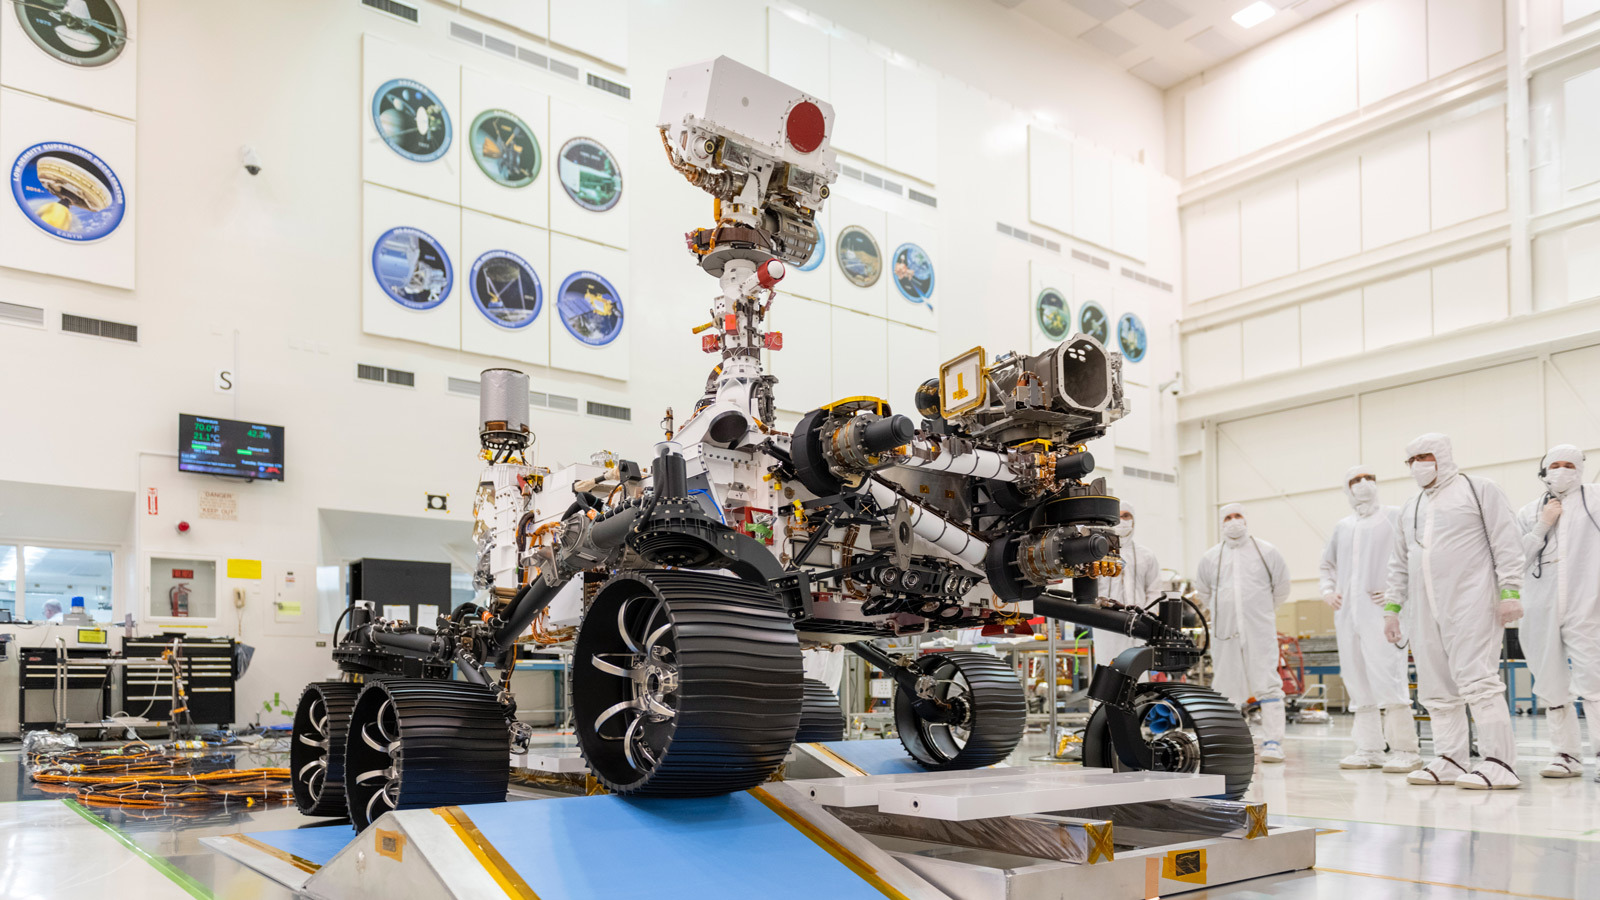
\includegraphics[height=9.5cm,keepaspectratio]{figures/perseverance.jpg}
%   \end{figure}
% \end{frame}
% 
% \begin{frame}[plain]
%   % As an environment, Mars offers unique challenges.
%   % For example, rocks can puncture the rover's wheels and sand can trap the rover.
%   % The rover relies on a combination of on-board and satellite based sensor data, which is often imperfect.
%   % Also, low-latency direct human control is impossible.
%   \begin{figure}
%   \centering
%   \vspace*{-1em}
%   \hspace*{-3em}
%   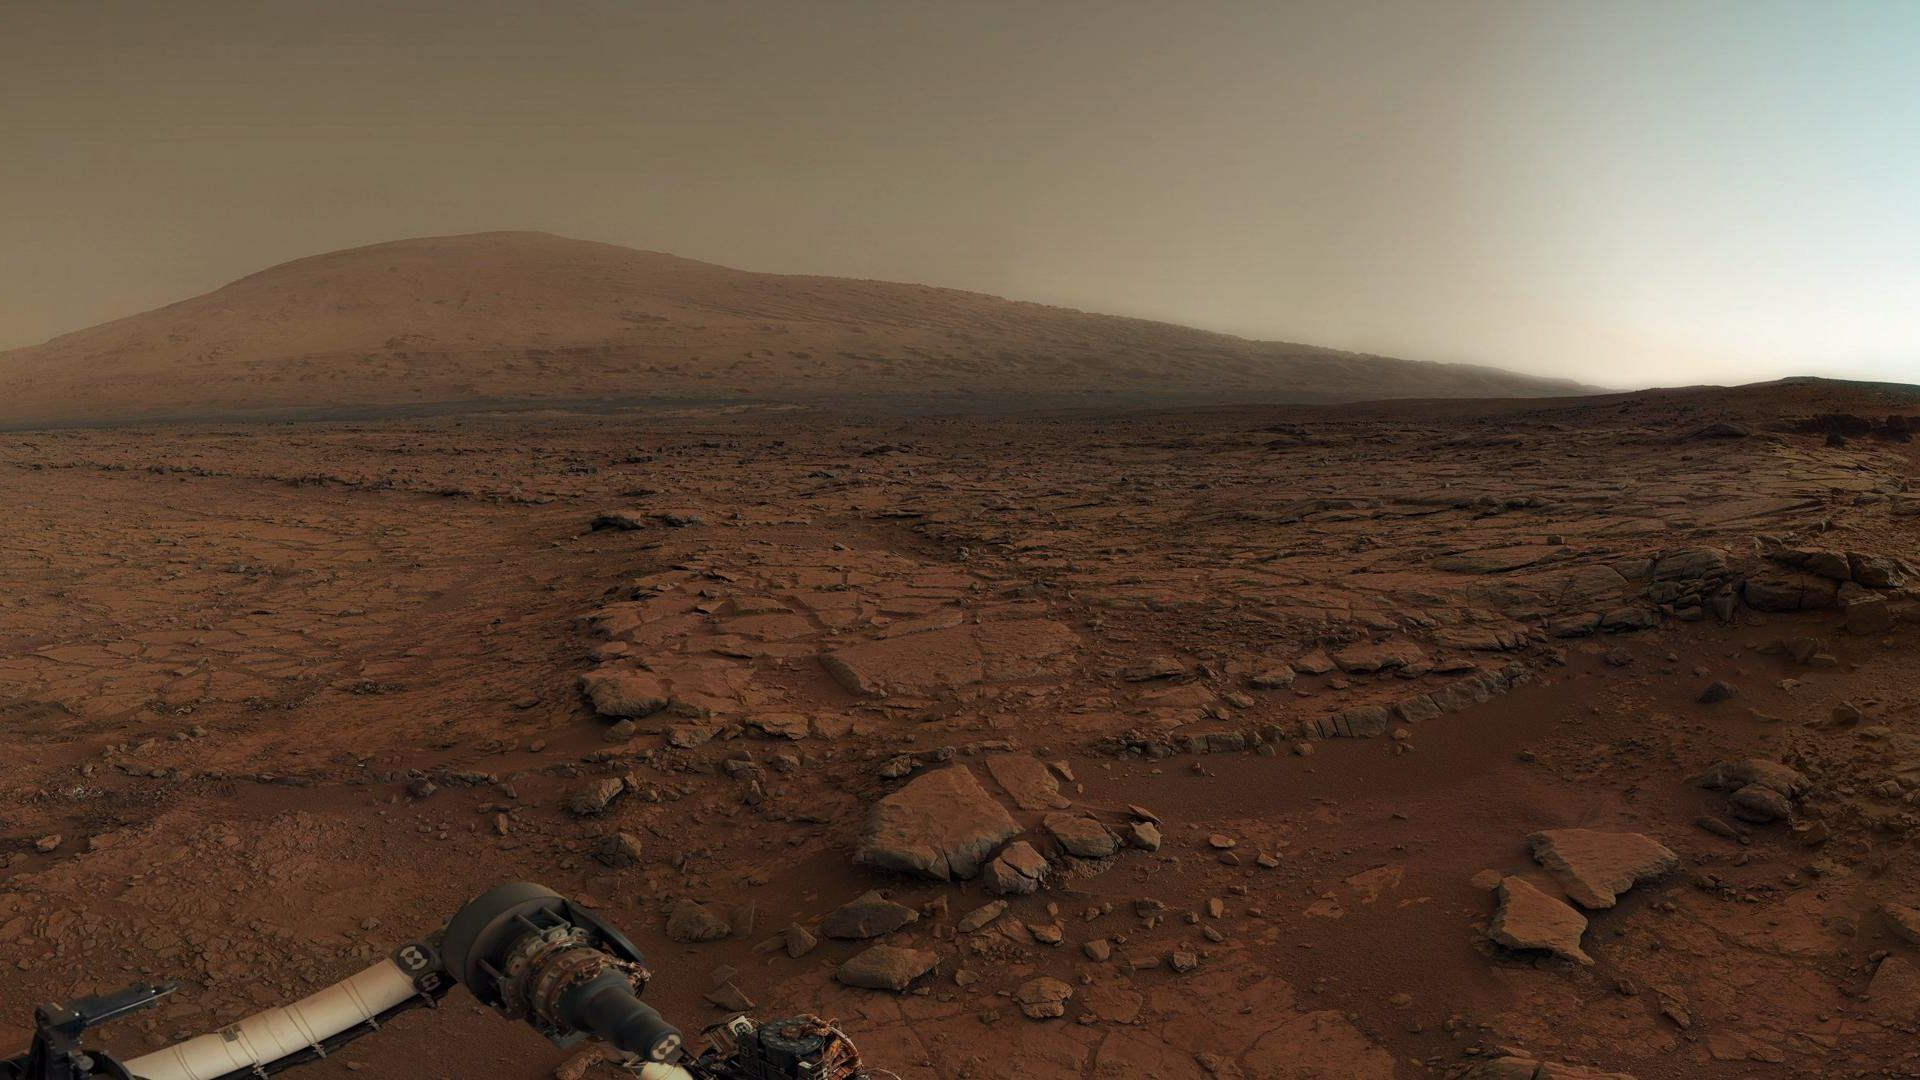
\includegraphics[height=9.5cm,keepaspectratio]{figures/mars_surface.jpg}
%   \end{figure}
% \end{frame}
% 
% \begin{frame}[plain]
%   % Alternatively, consider an environment like an Amazon warehouse.
%   % In contrast to mars, it is easy to navigate.
%   % The floor is perfectly smooth, the environment is mapped almost perfectly.
%   % Communication is fast, and it is easier to integrate advanced machine learning algorithms with robots.
%   % However, in an environment like this, there can be multiple robots, or even human-robot interaction.
%   % Humans, unlike robots, don't broadcast their telemetry, and can be unpredictable.
%   % So, robots must plan very carefully to avoid dangerous collisions.
%   % (pause)
%   % Considering these differences between Mars and an Amazon warehouse brings us to the main goal of this thesis.
%   \begin{figure}
%   \centering
%   \vspace*{-1em}
%   \hspace*{-3em}
%   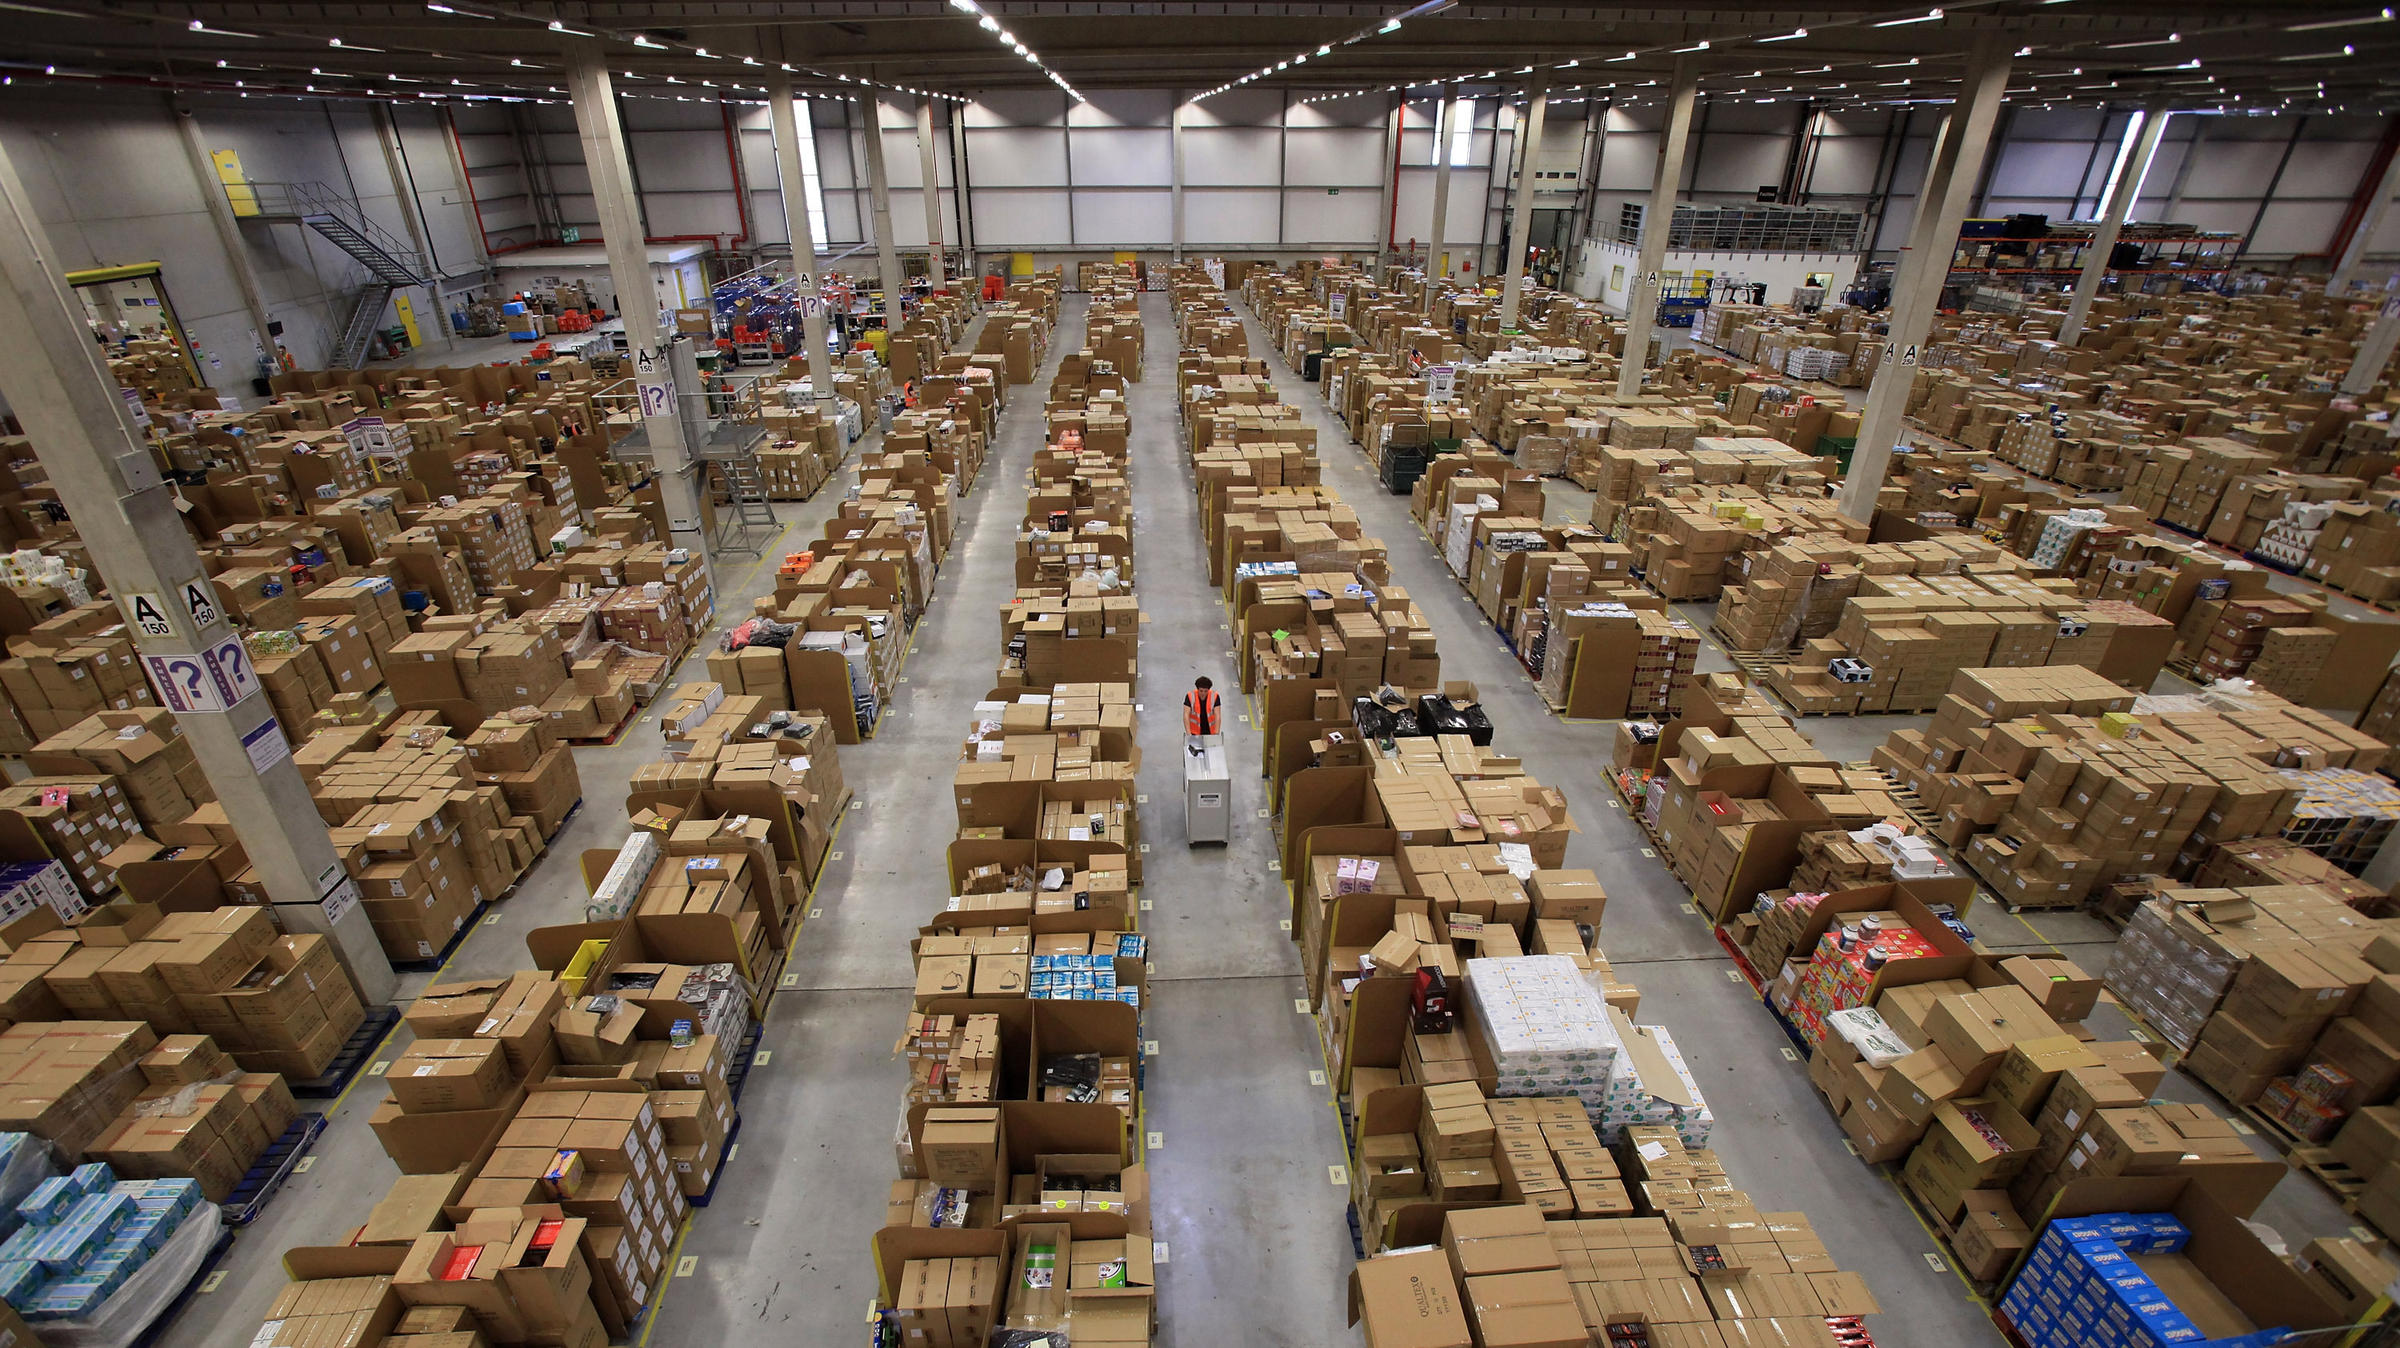
\includegraphics[height=9.5cm,keepaspectratio]{figures/warehouse.jpg}
%   \end{figure}
% \end{frame}
% 
% \begin{frame}{\white{Core Goals \& Concepts}}
%   % Conceptually, the focus of this thesis is on environment learning in robots.
%   %     Modern artificial intelligence is trying to move away from custom-engineering
%   %     In the context of this thesis, this means teaching robots to be generally proficient at new tasks.
%   %     But most importantly, this thesis focuses on the potential to specialize robots to particular environments.
%   % (pause)
%   % On the right, we have an image which I think is quite beautiful.
%   % This is a sketch from Darwin's notebook, presumably from when he first thought of evolution.
%   % It shows a tree depicting common ancestry and specialization.
%   \begin{columns}[T]
%       \begin{column}{.5\linewidth}
%             \vspace{-0.7em}
%             \emphasis{Learning}
%             \begin{itemize}
%               \item {\Medium Flexibility: adapt to new tasks}
%             \end{itemize}
%             \vspace{1em}
%             \emphasis{Generalization}
%             \begin{itemize}
%               \item {\Medium Learn overall task proficiency?}
%             \end{itemize}
%             \vspace{1em}
%             \emphasis{Specialization}
%             \begin{itemize}
%               \item {\Medium Learn environment details?}
%             \end{itemize}
%       \end{column}
%       \begin{column}{.5\linewidth}
%           \begin{figure}
%               \centering
%               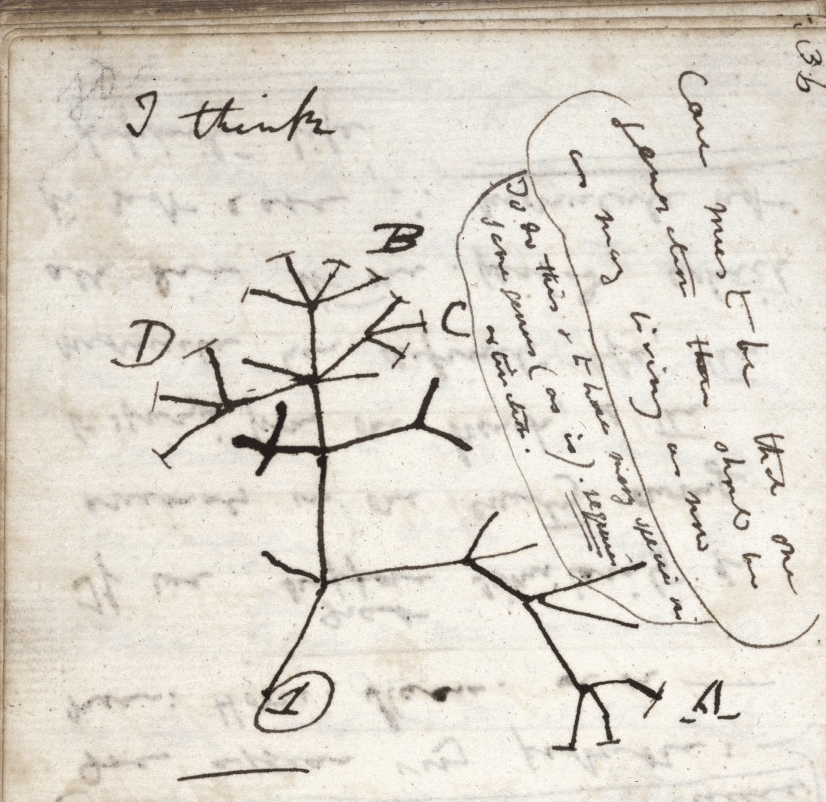
\includegraphics[height=5.5cm, keepaspectratio]{figures/i_think.png}
%               \caption{Where is this image from?}
%               \label{fig:i_think}
%           \end{figure}
%       \end{column}
%   \end{columns}
% \end{frame}
% 
% {
% \setbeamercolor{background canvas}{bg=white}
% \begin{frame}[plain]
%   % This is an artist's depiction of that same tree,
%   % In particular, it shows how specialization occurred over time.
%   % Bacteria have the oldest common ancestry.
%   % Mammals, on the other hand, are the most recent, and fill a vastly different niche.
%   % In between, there are incredibly diverse species within plants, fungi, fish, reptiles, and birds.
%   % This has led to at least 8.7 million species on earth
%   % And one can spend a lifetime for instance studying only plants
%   
%   % Ideally, this thesis would achieve the same specialization, but with..
%   \begin{figure}
%   \centering
%   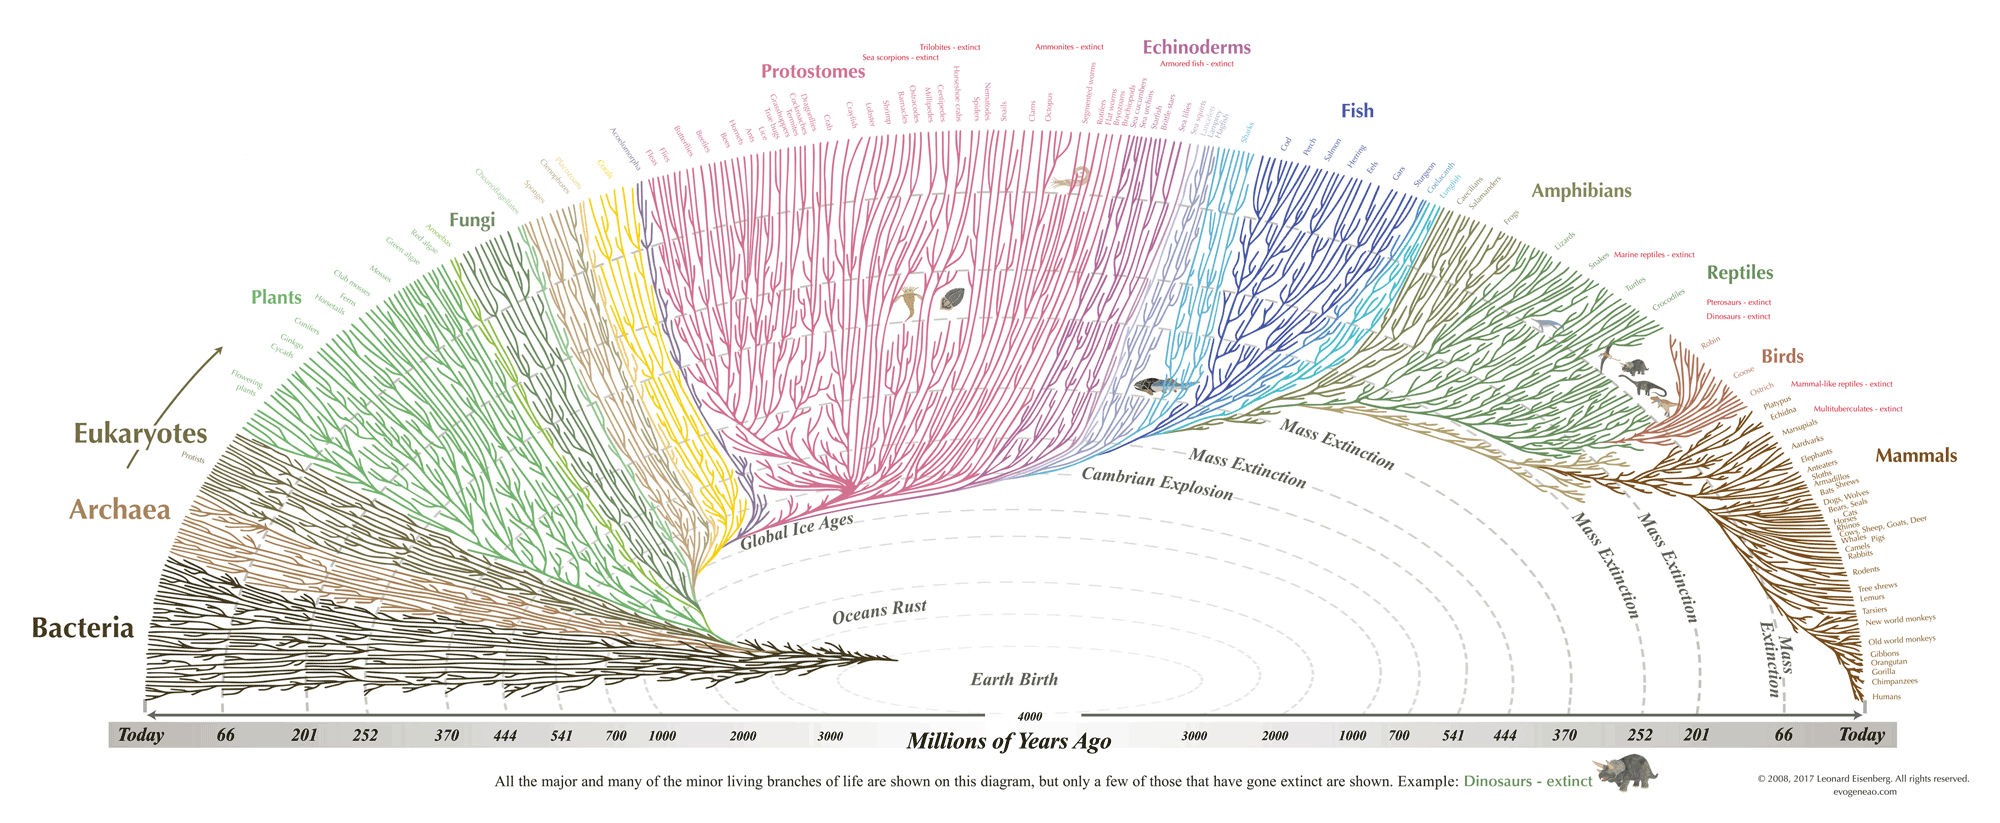
\includegraphics[width=1.0\linewidth,keepaspectratio]{figures/tree_of_life.png}
%   \end{figure}
%   \begin{center}
%       \emphasis{Natural evolution}
%   \end{center}
% \end{frame}
% }
% 
% \begin{frame}[plain]{}
%   % .. computer programs instead of biological species.
%   % Doing this is known as Evolutionary Programming
%   \centering
%   \vfill
%   \red{\fontsize{40}{50}\selectfont Computer Programs instead of species}
%   \vfill
%   \Huge Evolutionary Programming
% \end{frame}
% 
% \begin{frame}[plain]
%   % In this slide is a teaser figure showing an ancestry tree, where programs have evolved for special tasks.
%   \begin{figure}
%   \centering
%   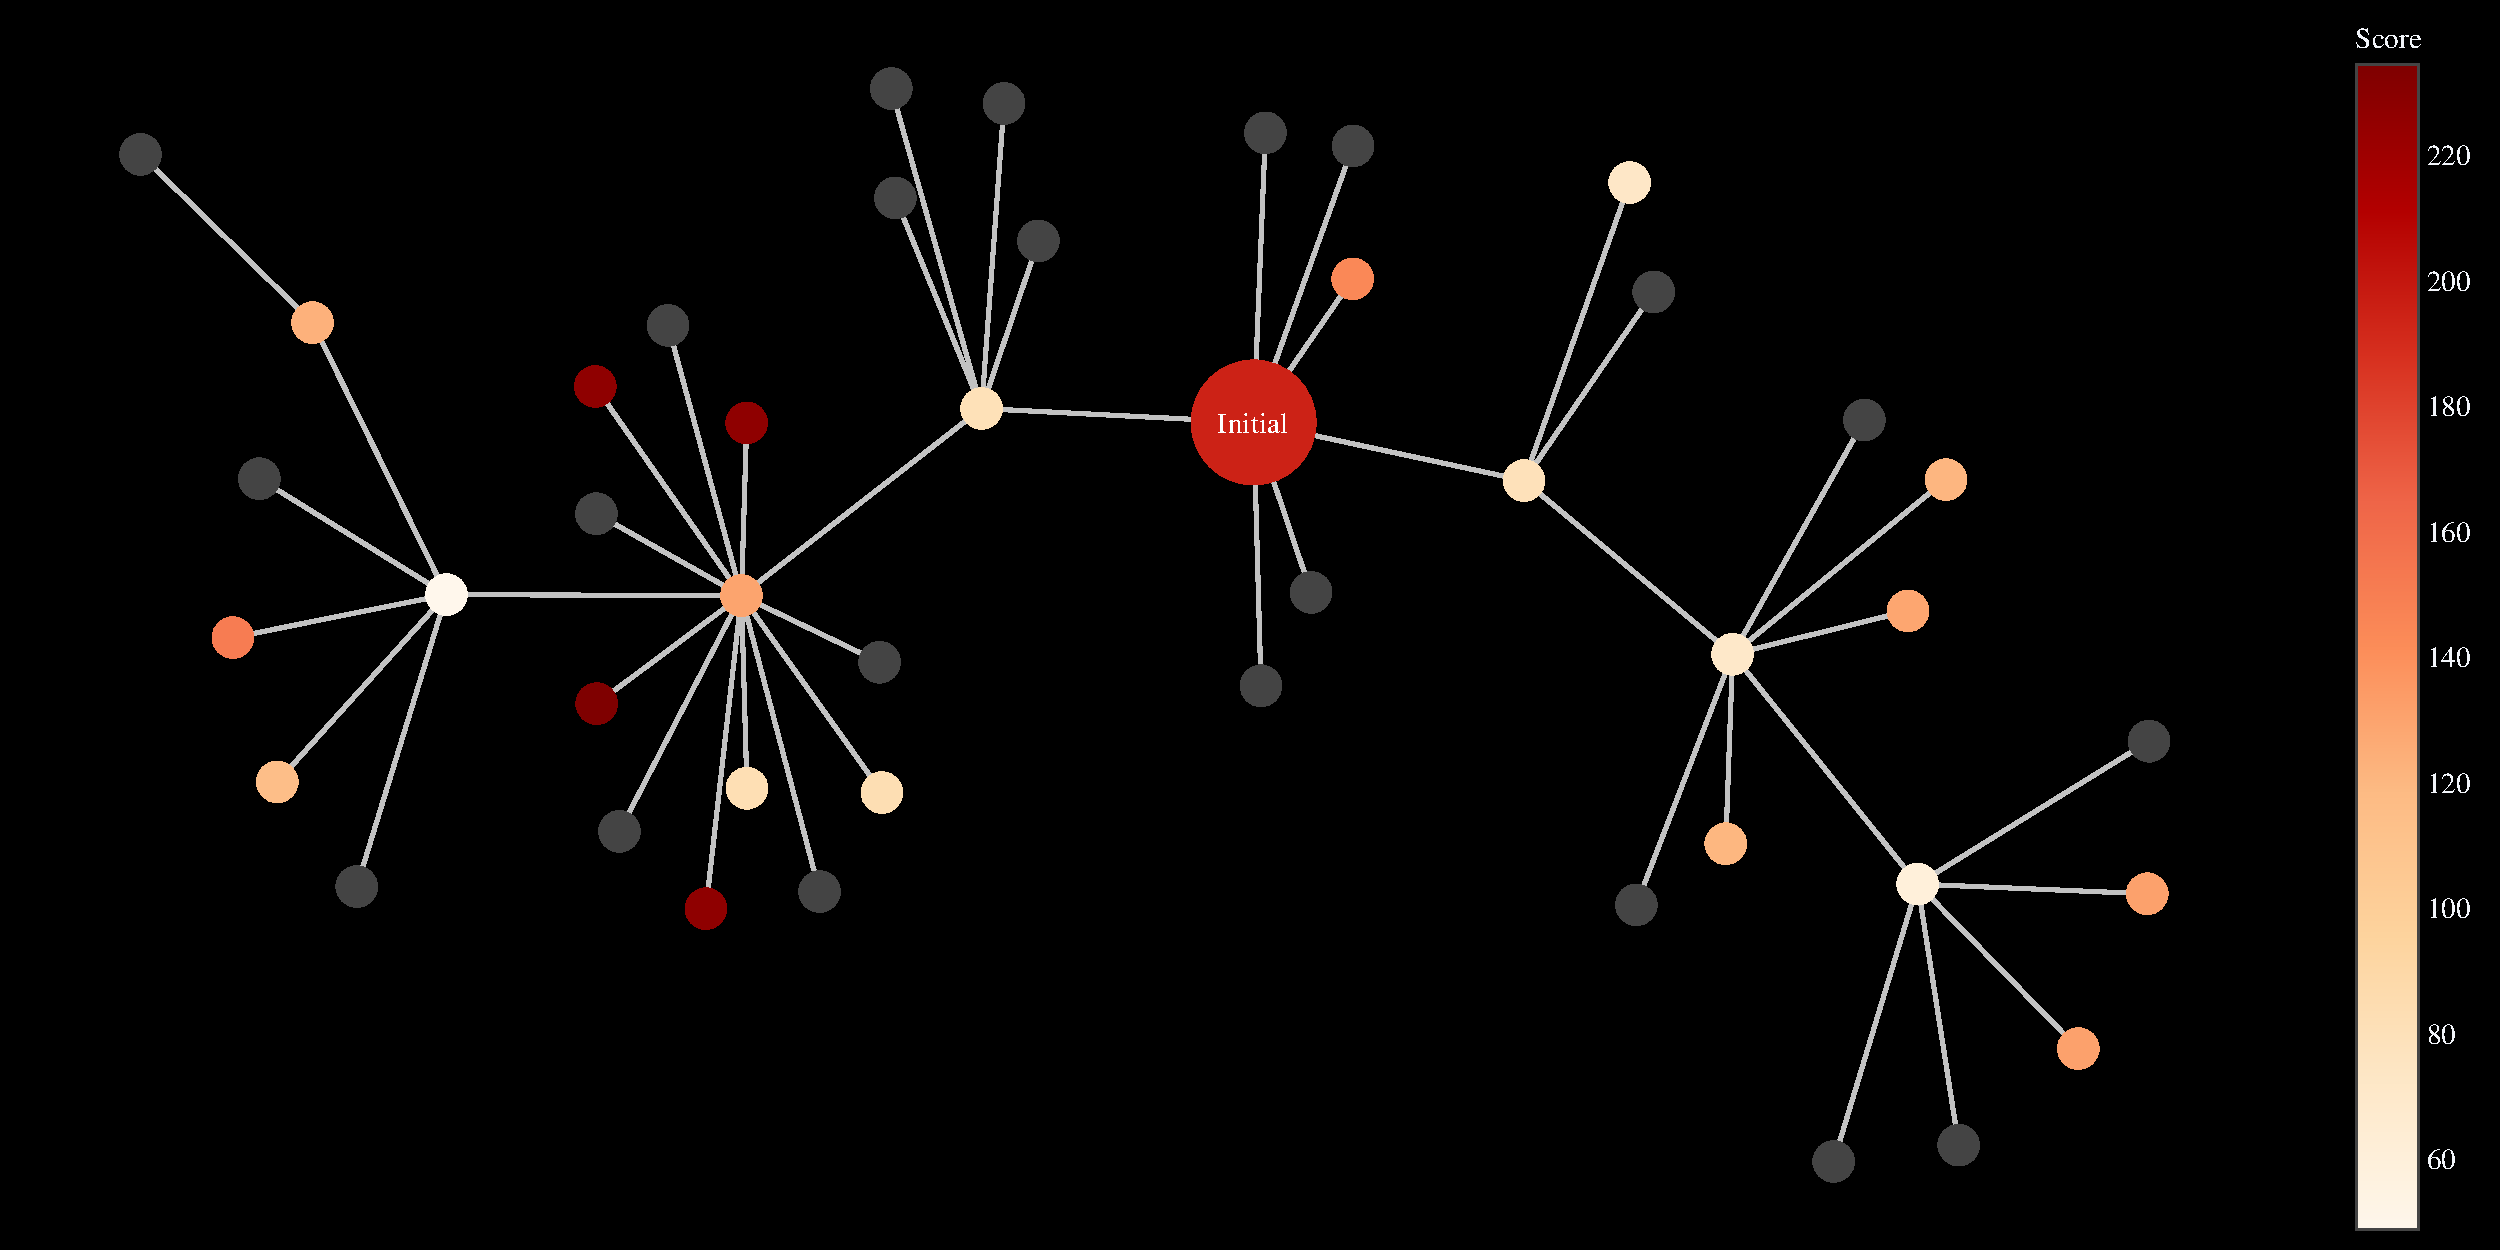
\includegraphics[width=1.0\linewidth,keepaspectratio]{figures/unlabeled_tree.pdf}
%   \end{figure}
%   \begin{center}
%   \emphasis{Evolved Computer Programs}
%   \end{center}
% \end{frame}
% 
% \begin{frame}[plain]{\white{Problems Considered}}
%   % In particular, the task this thesis considers is *Path Planning*
%   % Path planning is the task of finding a sequence of moves between points in space.
%   % For example, on the left is a 2 dimensional map of Milan, Italy, and a robot has been tasked with finding a path between the Orange dot and the Purple dot.
%   % Originally, this thesis focused on graph-based planning, where possible moves are specified in advance, in the form of a discrete graph.
%   % However, it has moved towards sampling-based planning, where possible moves are gathered by probing the environment.
%   % The methods described in this thesis work just as well dynamic (Mars) or multi-agent planning (Amazon), but these are left for future work. 
%   % They also have strong relations to symbolic regression or neural architecture search.
%   \begin{columns}[T]
%       \begin{column}{.5\linewidth}
%           \vspace{0.5cm}
%           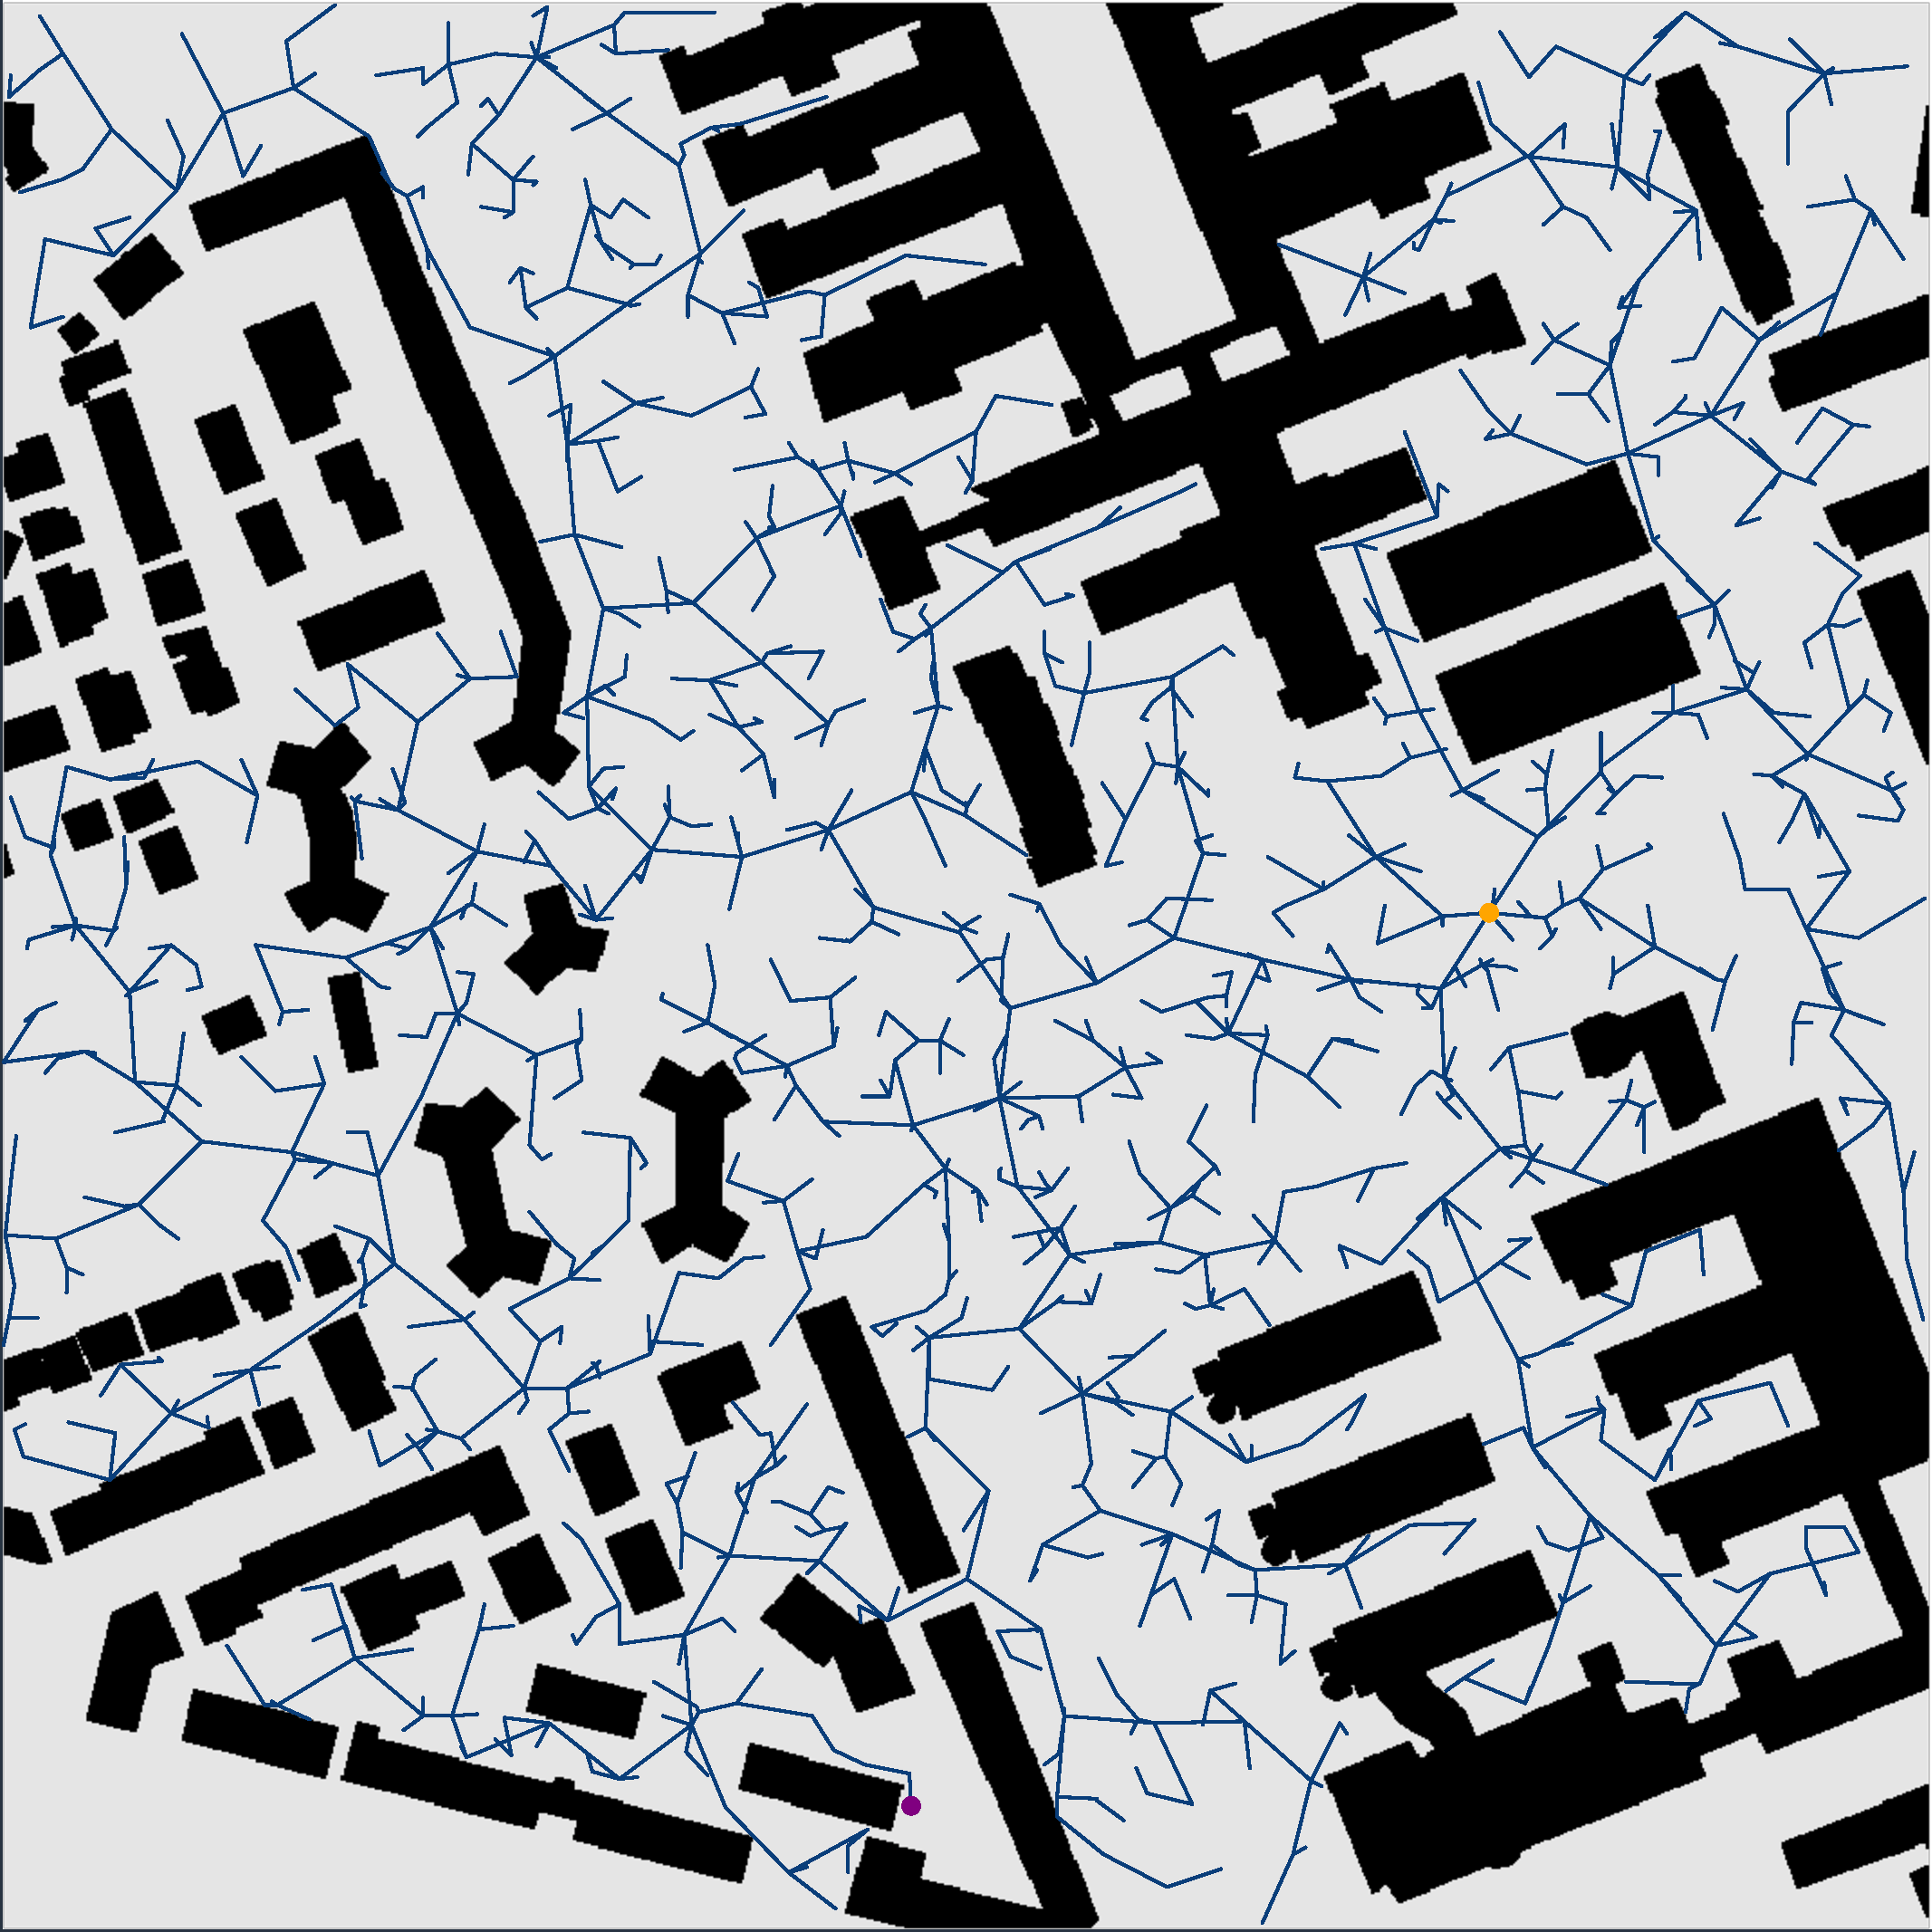
\includegraphics[width=1.0\linewidth, keepaspectratio]{figures/one_off.pdf}
%           \vfill
%       \end{column}
%       \hspace{1.0em}
%       \begin{column}{.5\linewidth}
%           \emphasis{Path Planning}
%           \begin{vfilleditems}
%               \item {\Large Graph-based}
%               \vspace{1em}
%               \item {\Large Sample-based \Medium (left)}
%               \vspace{1em}
%               \item {\color{grey} {\Large Dynamic (i.e. Mars)}}
%               \vspace{1em}
%               \item {\color{grey} {\Large Multiagent (i.e. Amazon)}}
%           \end{vfilleditems}
%           \vspace{1em}
%           {\color{grey} {\Large Symbolic Regression}}
%           \vspace{1em}
%           {\color{grey} {\Large Neural Arch. Search}}
%       \end{column}
%   \end{columns}
% \end{frame}
% 
% \begin{frame}[plain]{Graph search w/ Dijkstra \white{(New York)}}
%     % This image shows the behavior of a graph-based path planner, specifically Dijkstra's algorithm, on a map of New York.
%     % In this case, the streets are specified in advance, and a planning algorithm is asked to find a route from the bottom of New York to the top of New York
%     % Pink indicates roads that were considered
%     % Blank indicates unconsidered roads
%     % Yellow indicates the optimal path
%     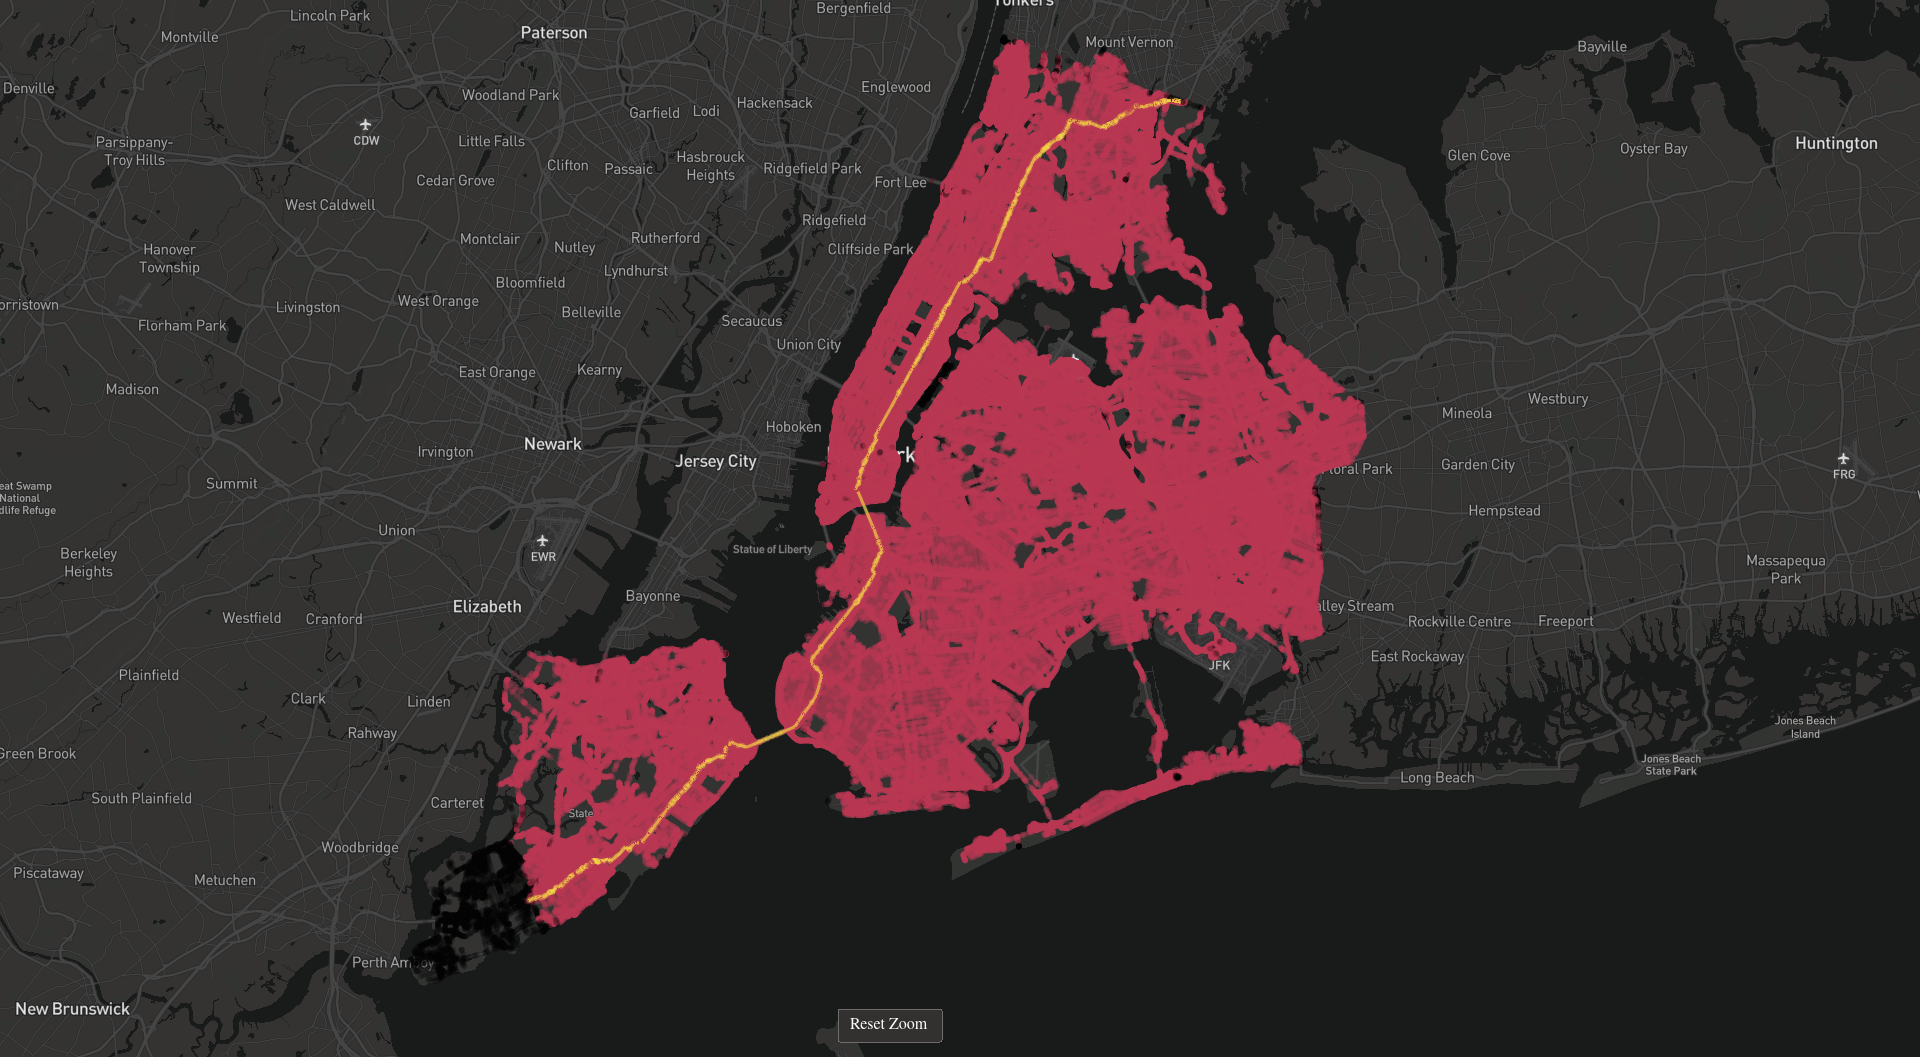
\includegraphics[width=1.0\linewidth, keepaspectratio, trim={0cm, 2cm, 1cm, 0.5cm}, clip]{figures/ny_graph_based.png}
% \end{frame}
% 
% \begin{frame}[plain]{Graph search w/ A* \white{(New York)}}
%     % However, the choice of algorithm can be a difference of millions of roads.
%     % This algorithm is A* with a geodesic heuristic.
%     % This means the algorithm knows a lower bound on how far it is from the goal at any time.
%     % In this thesis, I will demonstrate how it is possible to find similar improvements *automatically*
%     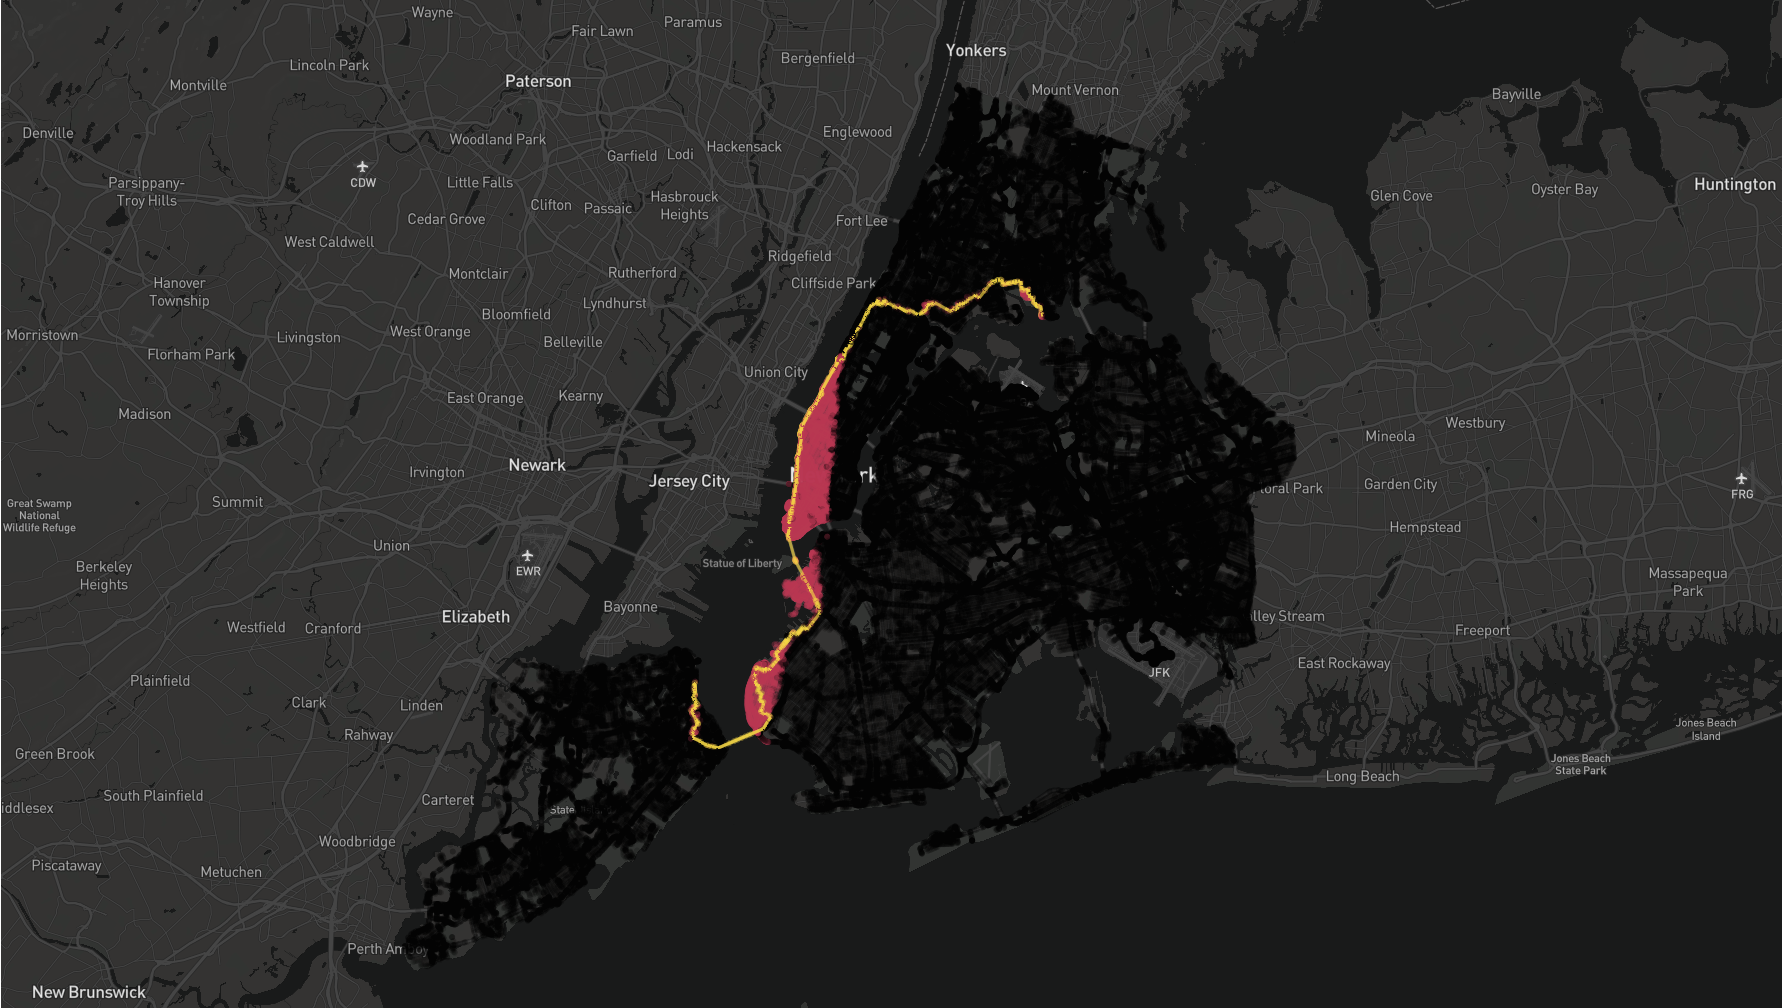
\includegraphics[width=1.0\linewidth, keepaspectratio, trim={0.5cm 1.5cm 0 2.5cm}, clip]{figures/ny_graph_based_geodesic.png}
% \end{frame}
% 
% \begin{frame}[plain]{Graph-based Algorithms \white{(Kiev, Ukraine)}}
%   % The graph-based portion of this thesis considered four relatively simple algorithms.
%   % These are Breadth first search, depth first search, Dijkstra's algorithm, and A* and its variants.
%   % If people are interested in more advanced algorithms, Hannah Bast of the University of Frieberg has an amazing paper on the subject.
%   % When using a service like Google Maps, it is more likely that it uses one of these more advanced algorithms.
%   % However, I leave these for future and ongoing work.
%   \begin{columns}[T]
%       \begin{column}{.4\linewidth}
%           \begin{vfilleditems}
%               \item {\Large Breadth-first (BFS)}
%               \item {\Large Depth-first (DFS)}
%               \item {\Large Dijkstra/A*}
%               \vspace{1em}
%               {\color{grey}
%               \item {\Large Goal-directed}
%               \item {\Large Separator-based}
%               \item {\Large Hierarchical}
%               \item {\Large Bounded Hop}
%               \item {\Large Hybrid Techniques}
%               \vspace{1em}
%               }
%               \item \red{\Large \cite{bast2016route}}
%           \end{vfilleditems}
%       \end{column}
%       \begin{column}{.6\linewidth}
%       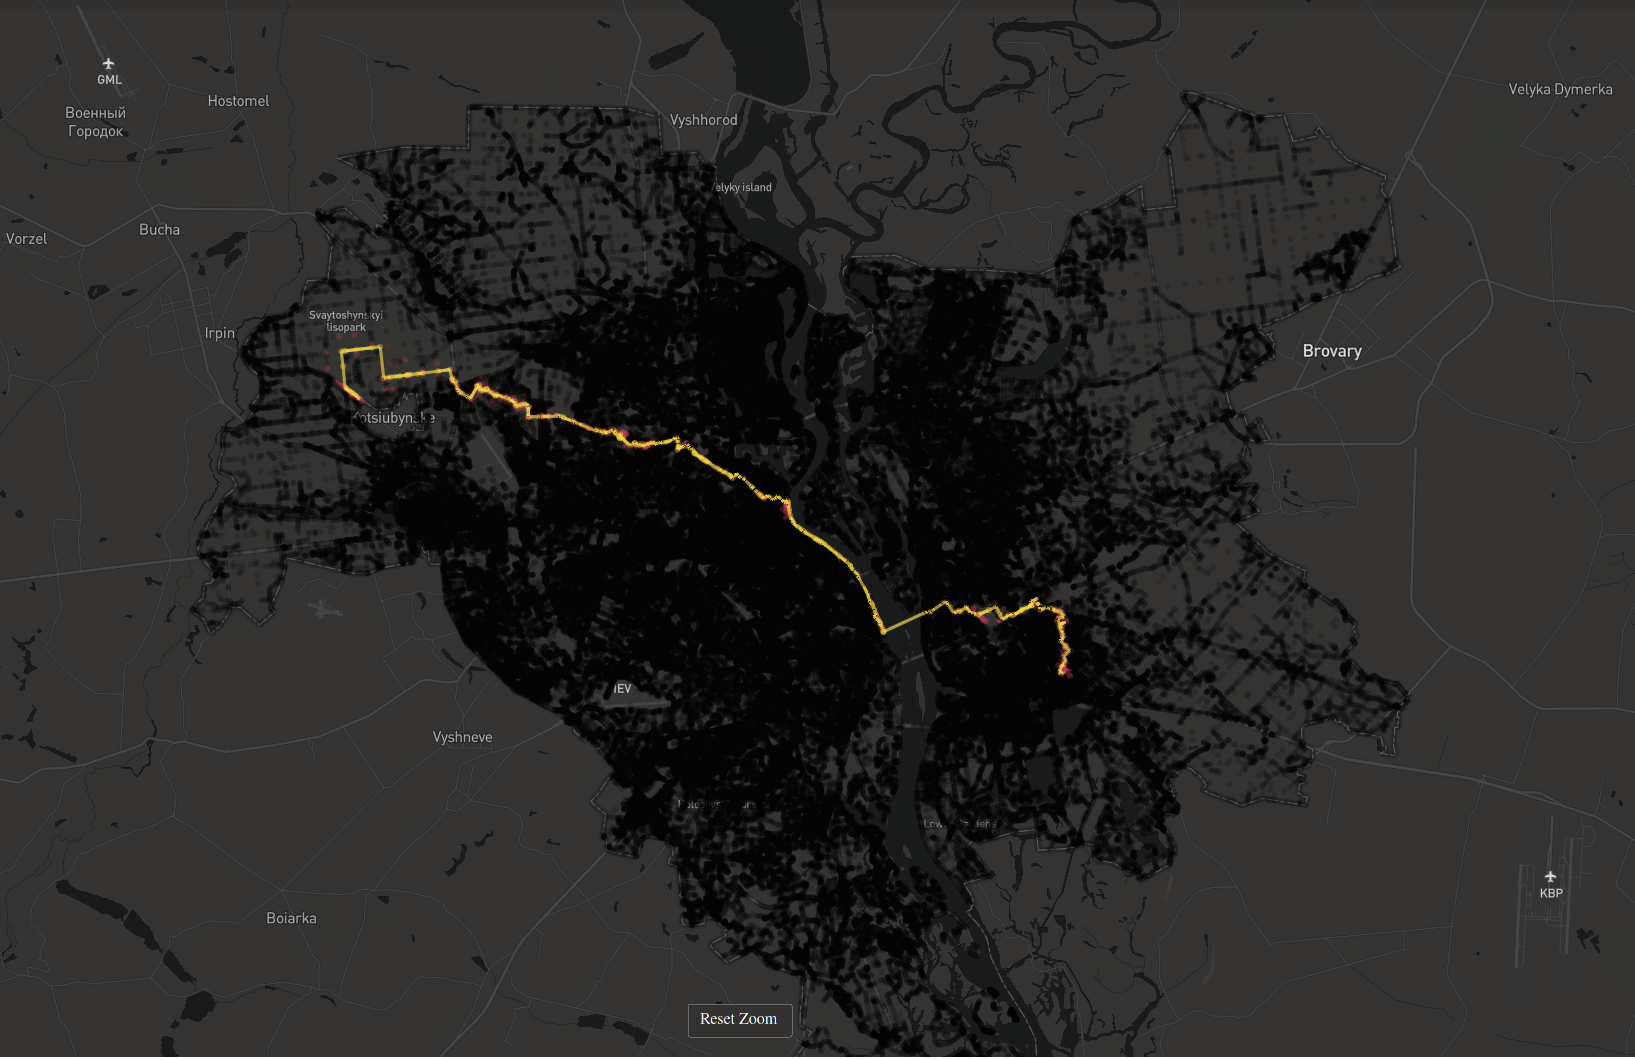
\includegraphics[height=0.9\textheight, keepaspectratio, trim={5cm 3cm 12cm 2cm}, clip]{figures/kiev.png}
%       \end{column}
%   \end{columns}
% \end{frame}
% 
% \begin{frame}[plain]{Sampling-based search \white{(Baldur's Gate)}}
%   % Next, there are sampling-based algorithms, which work by randomly sampling points in space.
%   % There are two main variants: Rapidly exploring random trees and probabilistic road-maps
%   % RRTs by far have the most variants, all of which address different conditions, like goal direction, a large amount of constrains, or a dynamic environment.
%   % Probabilistic road maps, on the other hand, (TODO)
%   % I focus mostly on simple RRT* variants
%   \begin{columns}[T]
%       \begin{column}{.35\linewidth}
%       \vspace{0.05\textheight}
%       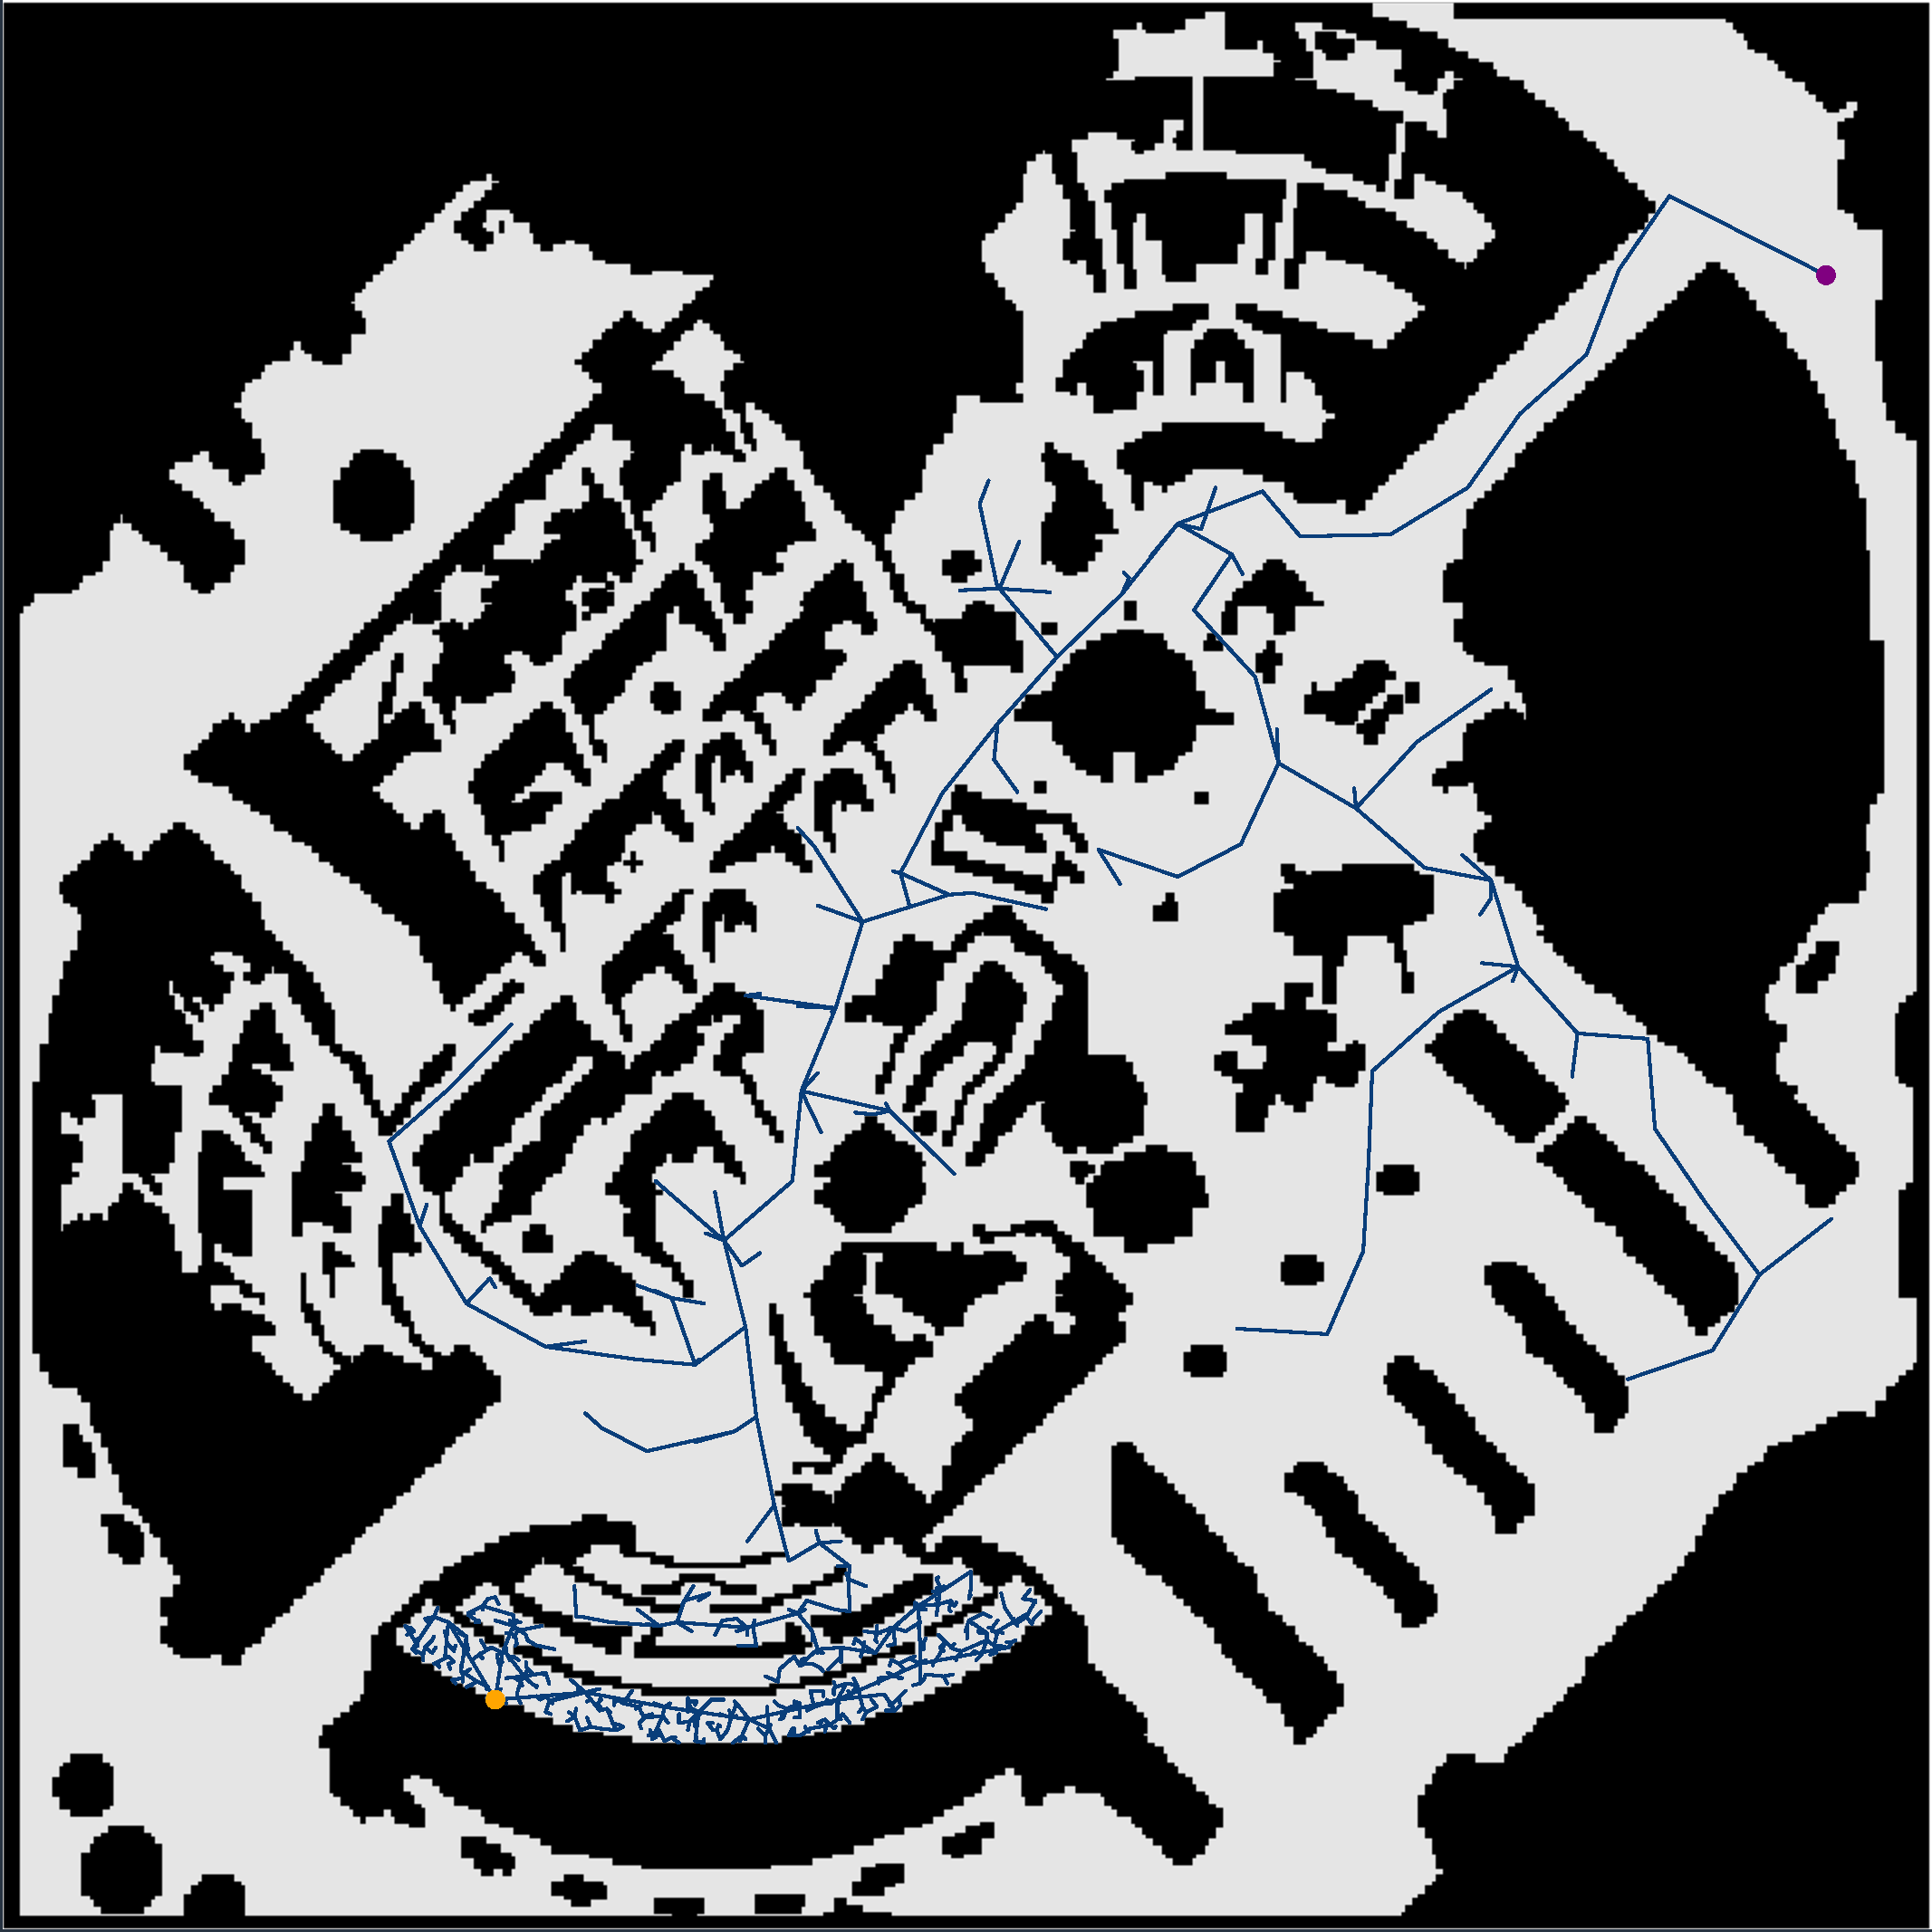
\includegraphics[height=0.7\textheight, keepaspectratio]{figures/baldurs_rrt_one_off.pdf}
%       \end{column}
%       \begin{column}{.65\linewidth}
%           \begin{vfilleditems}
%               \item {\Large Rapidly Exploring Random Trees \red{(RRTs)}}
%               \begin{itemize}
%                   \item RRT, RRT*, Informed RRT*
%                   \item Multi-phase
%                   \item RRT-Blossom
%                   \item Dynamic RRT* (RT-RRT*, RRTX, RRT#)
%               \end{itemize}
%               \vspace{1em}
%               \item {\Large Probabilistic Road Maps \red{(PRMs)}}
%               % \item {\Large \color{grey} Potential Fields}
%           \end{vfilleditems}
%       \end{column}
%   \end{columns}
% \end{frame}
% 
% \begin{frame}[plain]{RRT* \white{(Baldur's Gate)}}
%     % The basic principle behind RRTs is *Voronoi Regions*
%     % This figure shows the voronoi regions (in orange)
%     %   and convex hull (in pink) of an RRT* run
%     % Essentially, a new point is sampled, it will be connected to
%     %   its nearest neighbor. Voronoi regions represent which node
%     %   is nearest to an *area* of the map.
%     % The convex hull shows the outer perimeter of the explored space
%     Intentionally blank
%     % 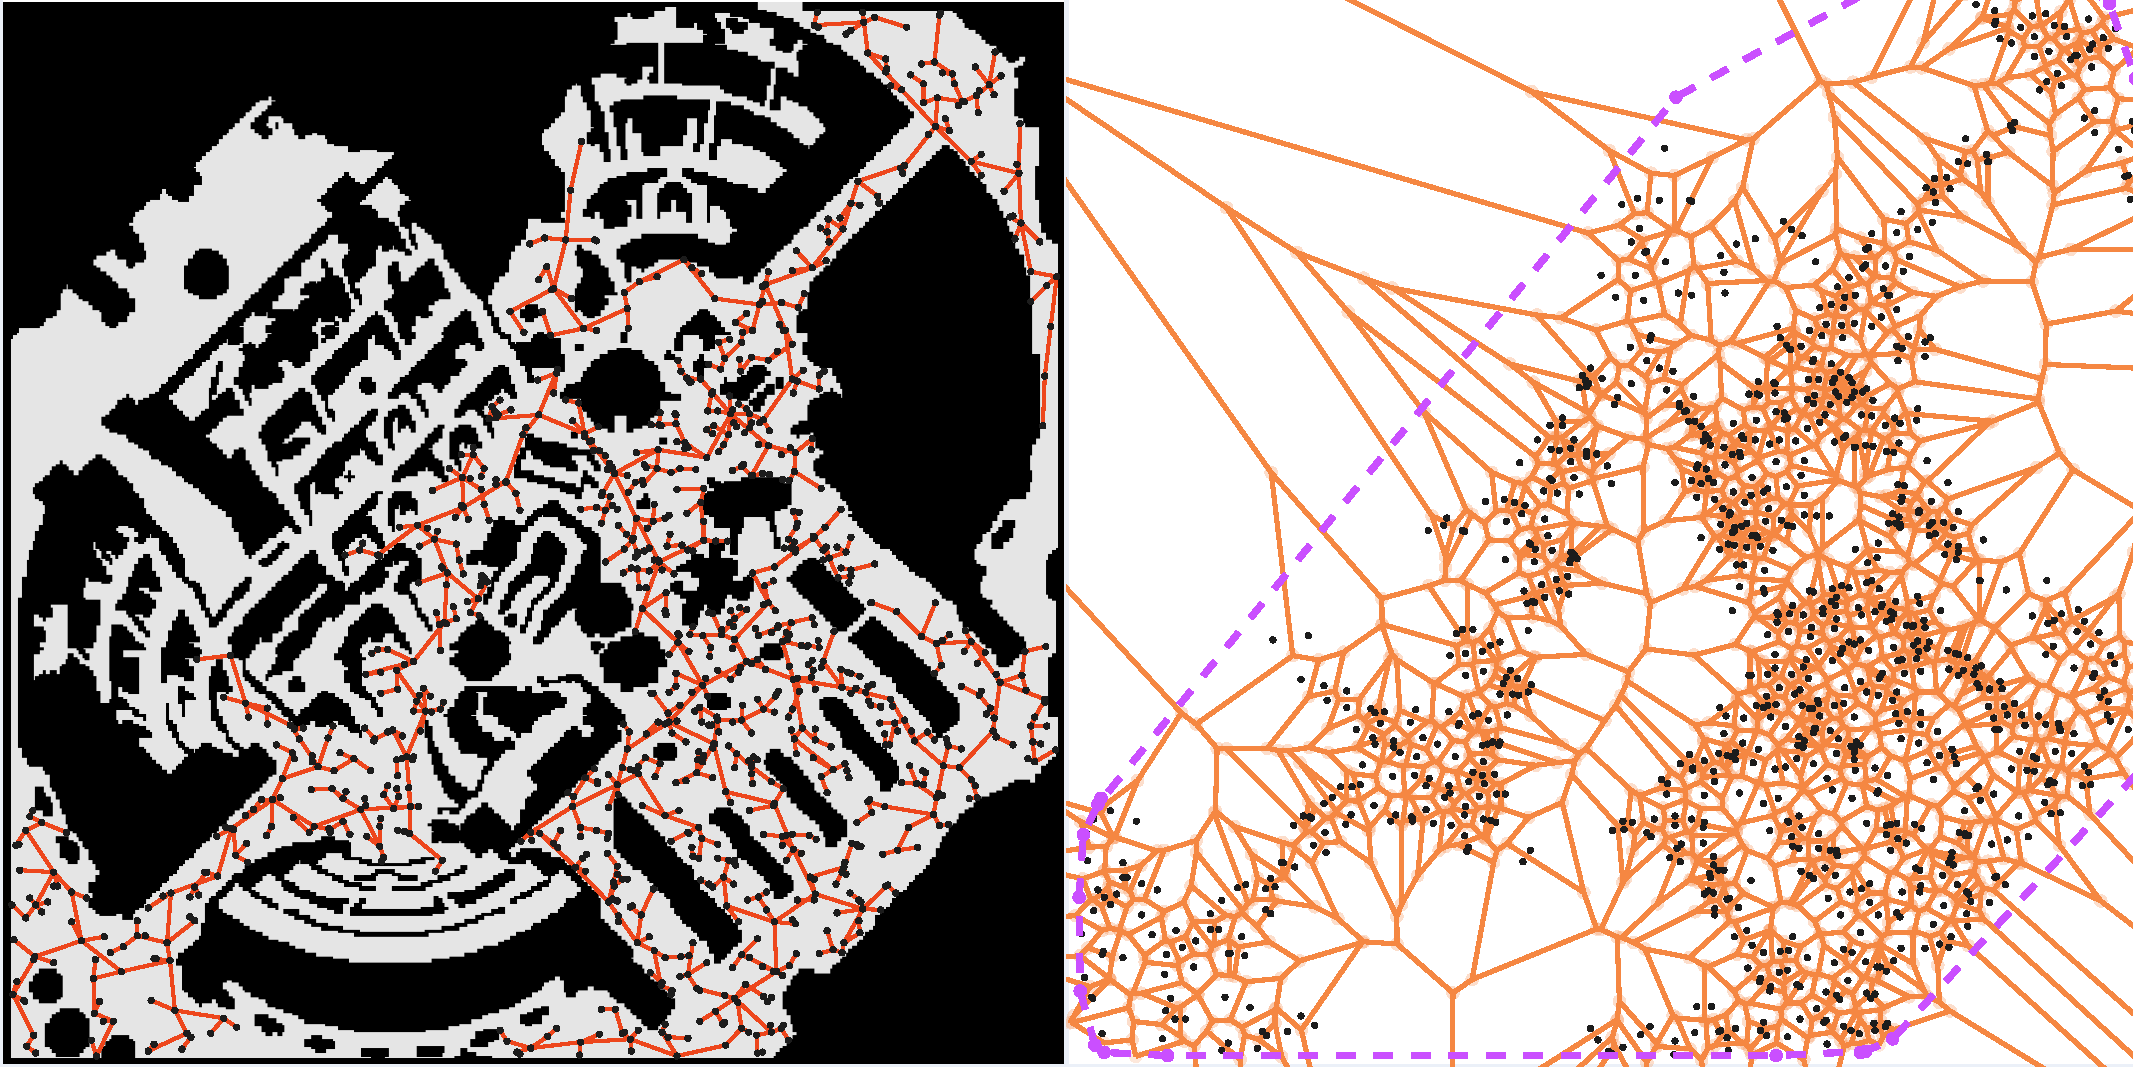
\includegraphics[width=1.0\linewidth, keepaspectratio]{figures/baldurs_1k_explorer.pdf}
% \end{frame}
% 
% \begin{frame}{Maps Overview {\Medium \color{white}( \cite{sturtevant2012benchmarks})}}
%     % Here is an overview of the various 2D maps considered in this thesis
%     % This includes maps from video games, such as:
%     %   - Baldur's Gate
%     %   - Dragon Age
%     %   - World of Warcraft
%     %   - Starcraft
%     % However, it also includes obstacle maps of large cities, such as:
%     %   - Boston, Shanghai, Milan
%     % Finally, it includes several mazes, and even some Amazon warehouses
%     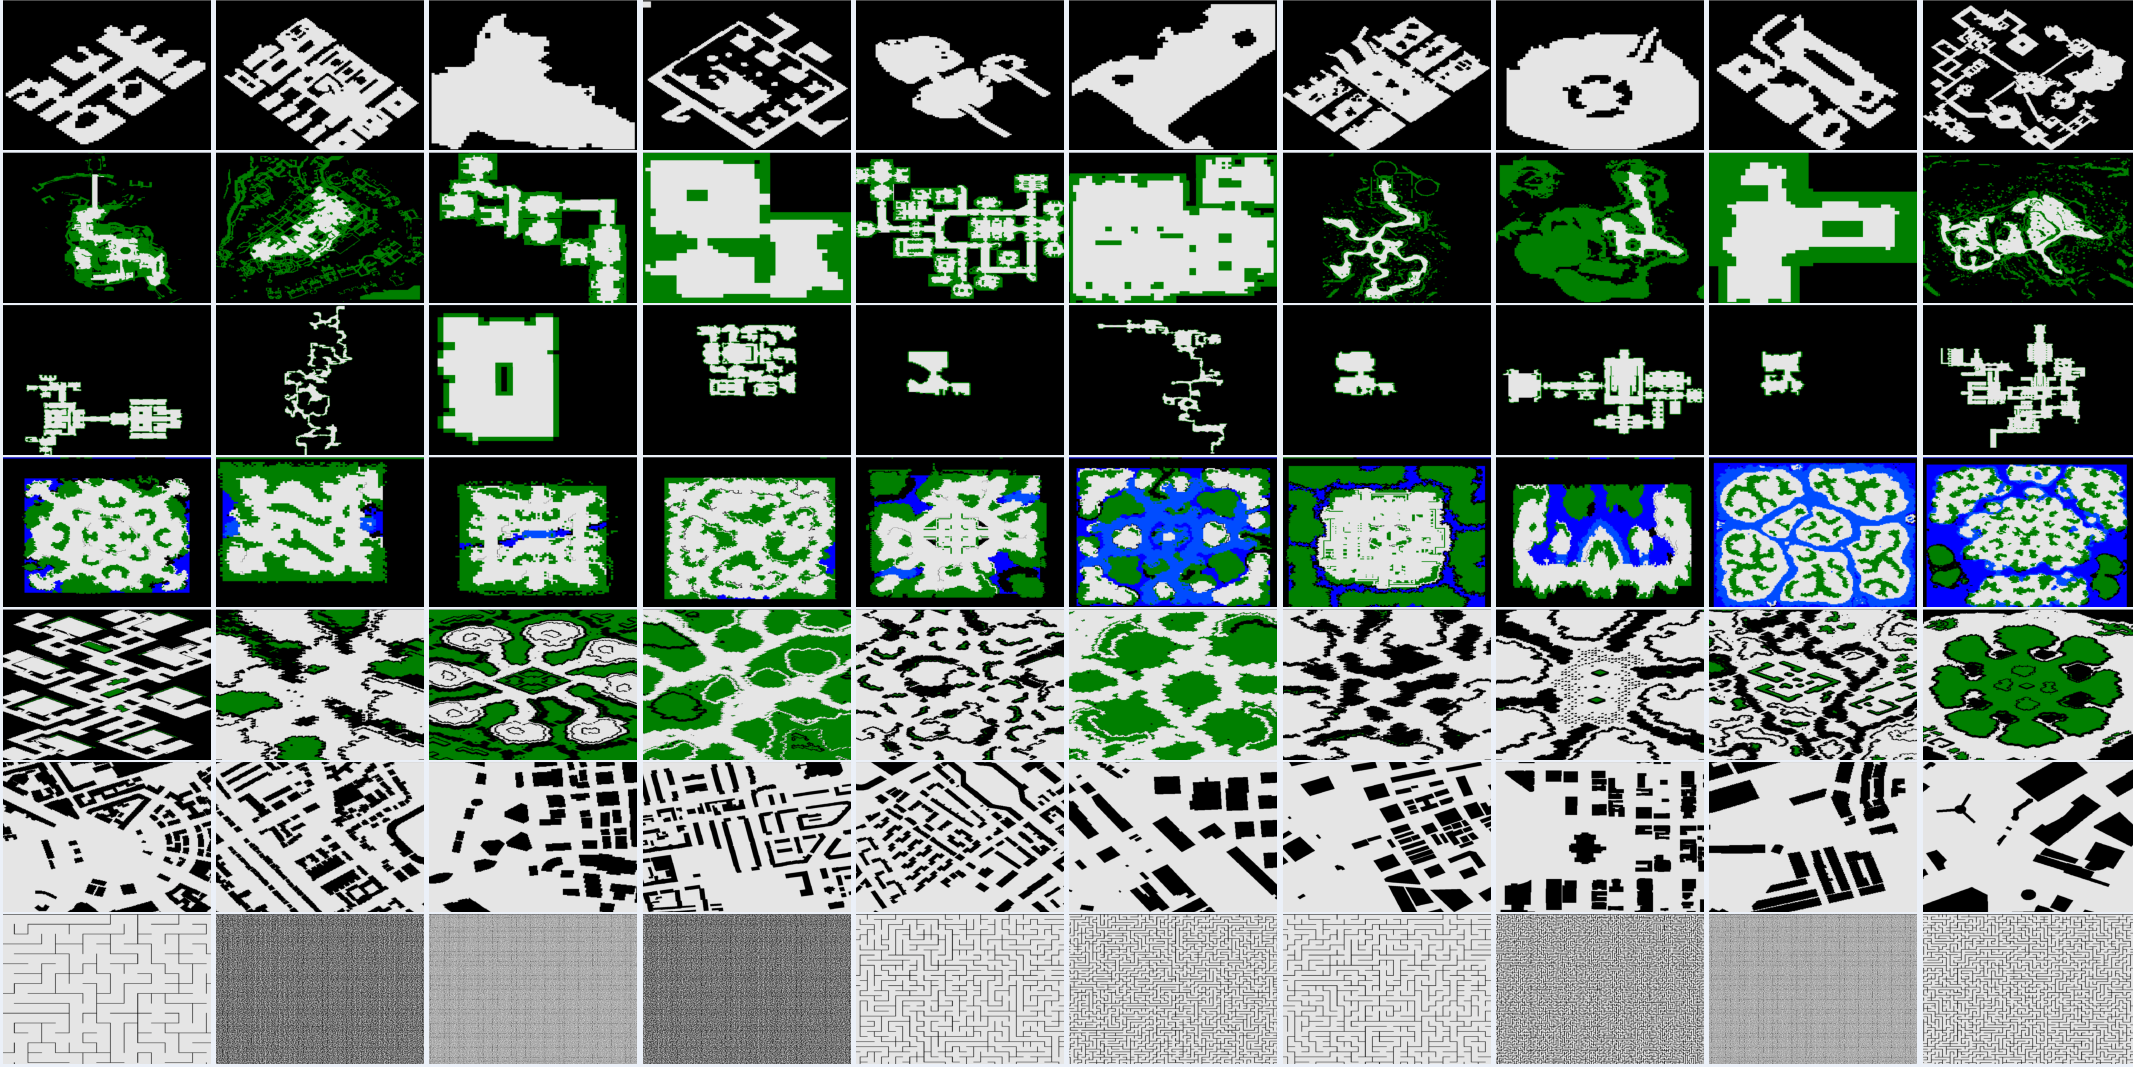
\includegraphics[width=0.95\linewidth, keepaspectratio]{figures/show_maps_overview.pdf}
% \end{frame}
% 
% \begin{frame}{Maps Detail {\Medium \color{white}( \cite{sturtevant2012benchmarks})}}
%     % Here, we see various maps in closer detail.
%     % Many maps in this dataset have unique characteristics.
%     % For example, this Shanghai map, or the bottom-left Dragon Age map are both relatively open.
%     % In contrast, the Boston map and Starcraft: Frozen Sea map are cluttered.
%     % The Baldur's gate map, the maze, and the Dragon Age mansion map all have narrow corridors.
%     % Because each map has it's own characteristics, the goal of this thesis is to specialize algorithms to each of them.
%     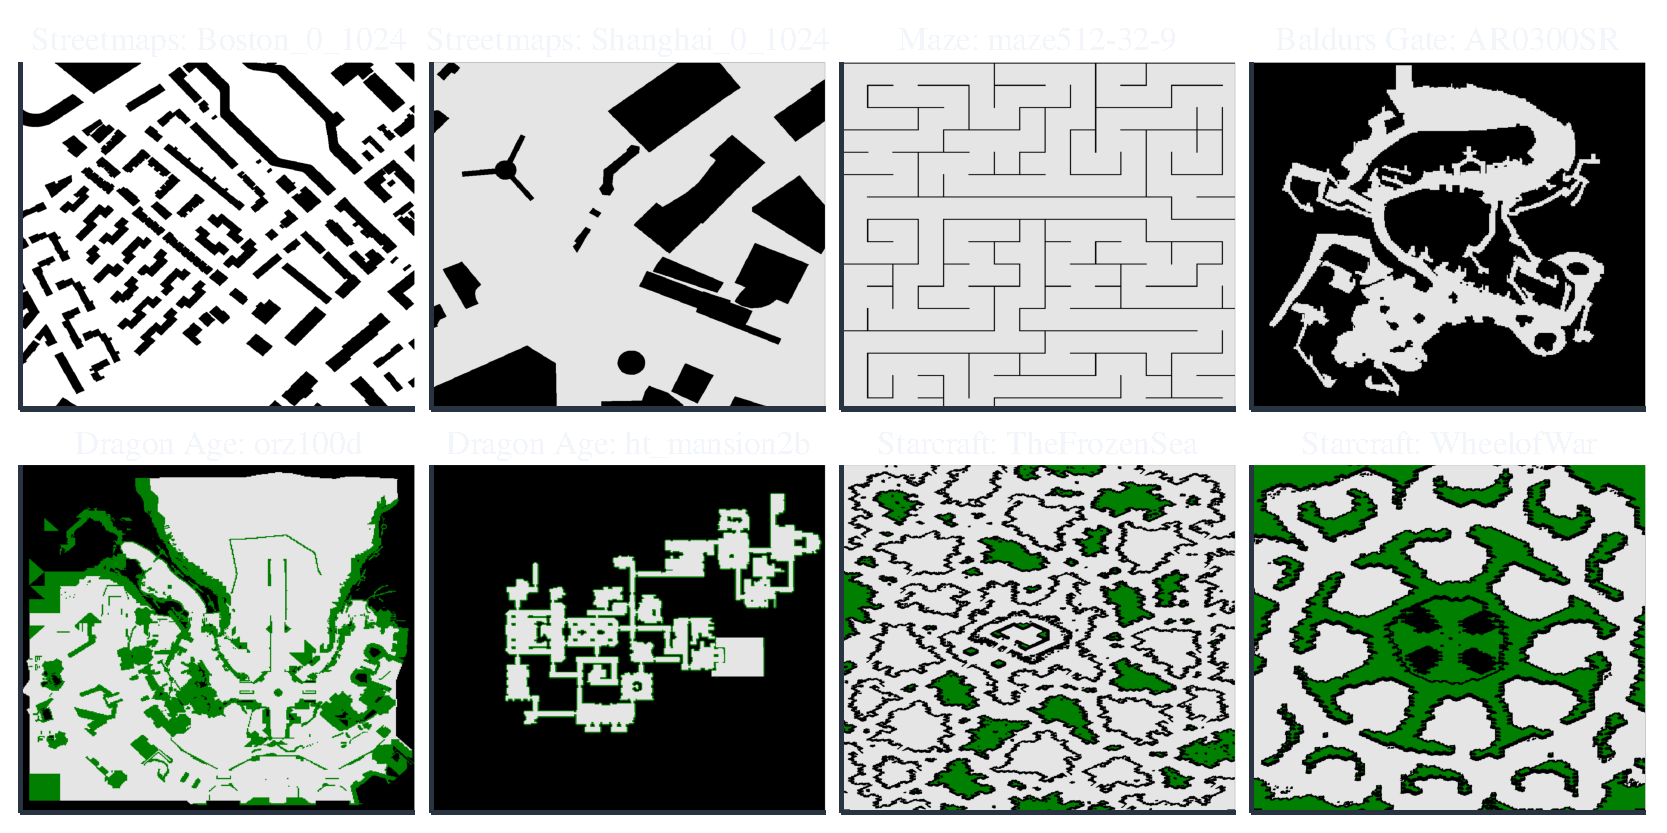
\includegraphics[width=1.0\linewidth, keepaspectratio]{figures/show_maps.pdf}
% \end{frame}
% 
% \begin{frame}{Specialization Results}
%   % Here is a teaser figure showing the potential for specialization.
%   % Four experiments were run on Boston, Baldur's Gate, Dragon Age, and Starcraft maps.
%   % The Boston planner runs relatively well
%   % The Baldurs Gate Planner runs relatively well
%   % The dragon age planner does not. I address this later on.
%   % The starcraft planner does exceptionally well given a difficult problem.
%   % That brings us to the methods section of this thesis.
%   \begin{columns}[T]
%       \begin{column}{.6\linewidth}
%       \centering
%       \vspace{-1em}
%       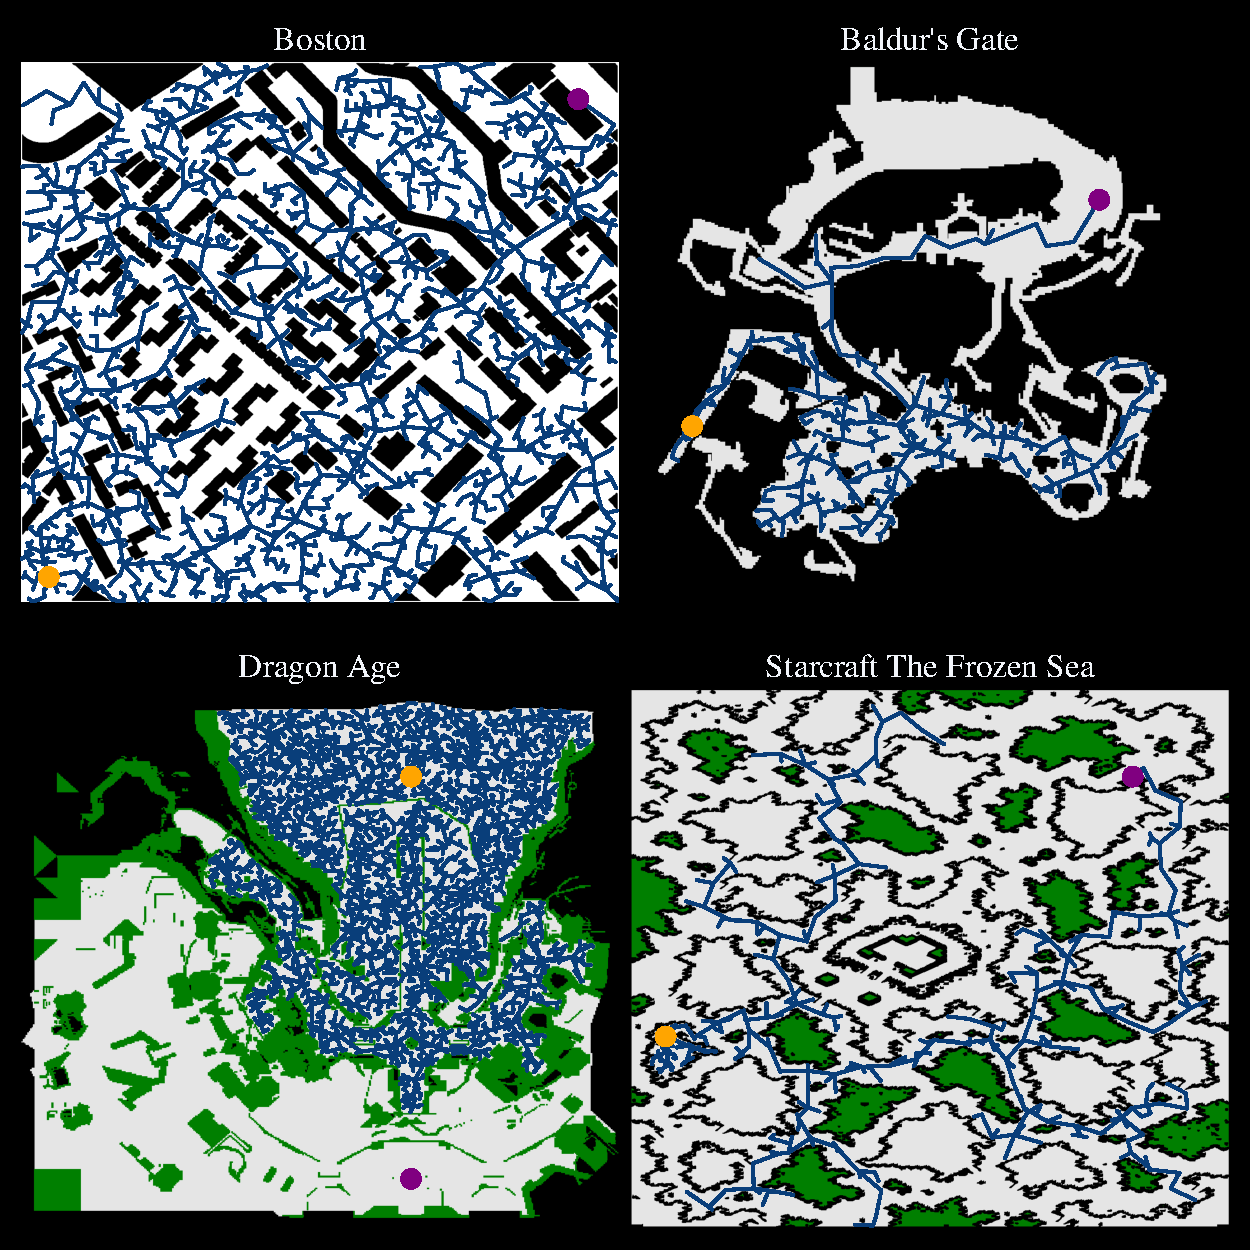
\includegraphics[height=0.9\textheight]{figures/learned2.pdf}
%       \end{column}
%       \begin{column}{.4\linewidth}
%       \centering
%       \epigraph{
%       There is no “silver bullet” algorithm for solving all path planning problems. Heuristics that lead to massive speed-up in one scenario might be detrimental in others. Also, algorithmic parameters are mostly ad-hoc and correctly tuning them to a \red{specific environment} might drastically increase performance.
%       }{\textit{
%       Nikolaus Correll
%       }}
%       \end{column}
%   \end{columns}
% \end{frame}
% 
% \begin{frame}[plain]{}
%   % Shown here is the mandelbrot set.
%   % The mandelbrot set is relevant, because it brings us to Andrey Kolmogorov, an important figure in *program synthesis*
%   % The mandelbrot set is important because it can be generated with a short computer program
%   %   but generates an image which takes up significantly more space.
%   % In other words, the mandelbrot set is an ideal example of *compression*
%   % Kolmogorov considered program synthesis for *compression*, and his central result was this:
%   \begin{figure}
%   \vspace*{-4em}
%   \hspace*{-4em}
%   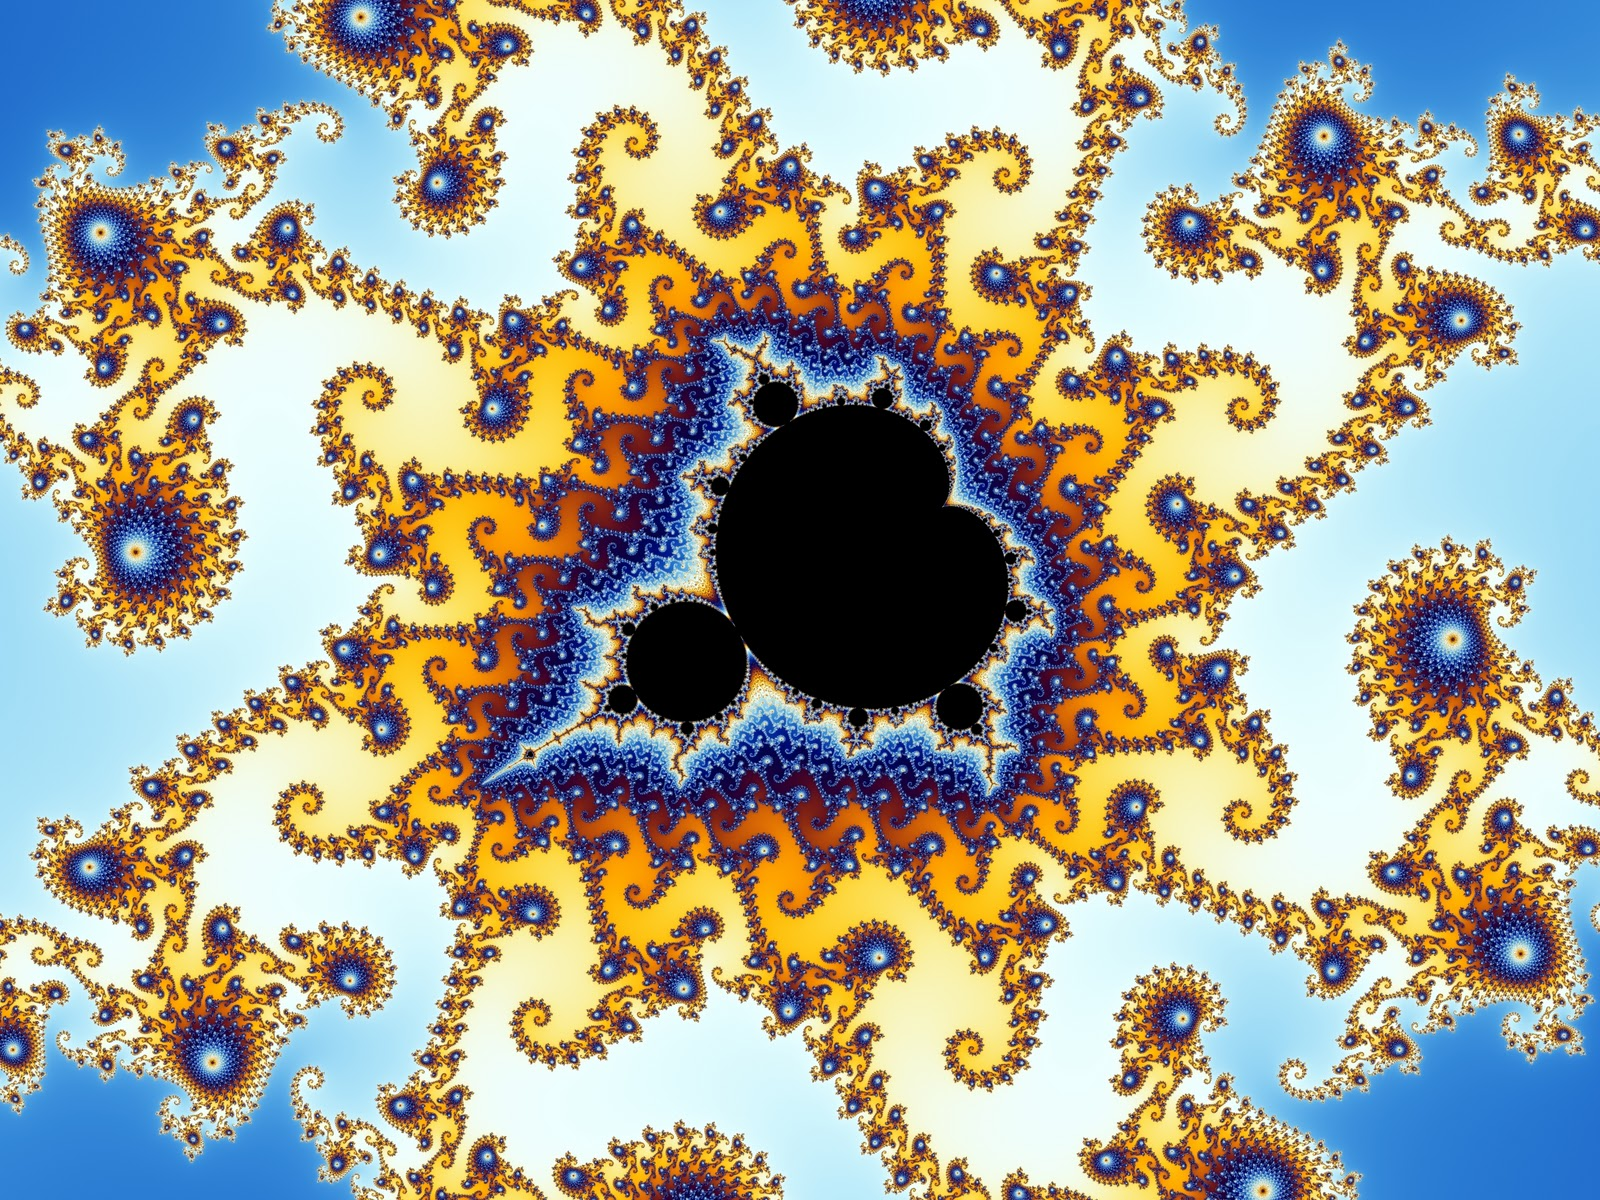
\includegraphics[width=1.2\linewidth,keepaspectratio]{figures/mandelbrot_2.jpg}
%   \end{figure}
% \end{frame}

\begin{frame}[plain]{\white{Program Synthesis}}
  % Searching program space exhaustively is impossible, because of Turing's halting problem.
  % (pause)
  % However, the work of Lenat and Schmidhuber explore 
  %   "universal problem solving".
  %   If program space can be traversed efficiently, universal problem solvers can be created.
  % This is the high-level theory and motivation behind program synthesis.
  \begin{columns}[T]
      \begin{column}{.5\linewidth}
          \vspace{1em}
          \emphasis{Kolmogorov}
          \newline
          \begin{itemize}
              \item Searching program space \textit{exhaustively} is impossible (\cc{Turing:} Halting Problem)
          \end{itemize}
          \onslide<2->{
          \emphasis{Lenat}
          \newline
          \begin{itemize}
              \item Universal problem solvers
          \end{itemize}
          \emphasis{Schmidhuber}
          \newline
          \begin{itemize}
              \item Optimal Ordered Solvers
          \end{itemize}
          }
      \end{column}
      \begin{column}{.5\linewidth}
          \begin{figure}
              \vspace{-3.5em}
              \hspace*{1.3em}
              \rotatebox[origin=c]{-90}{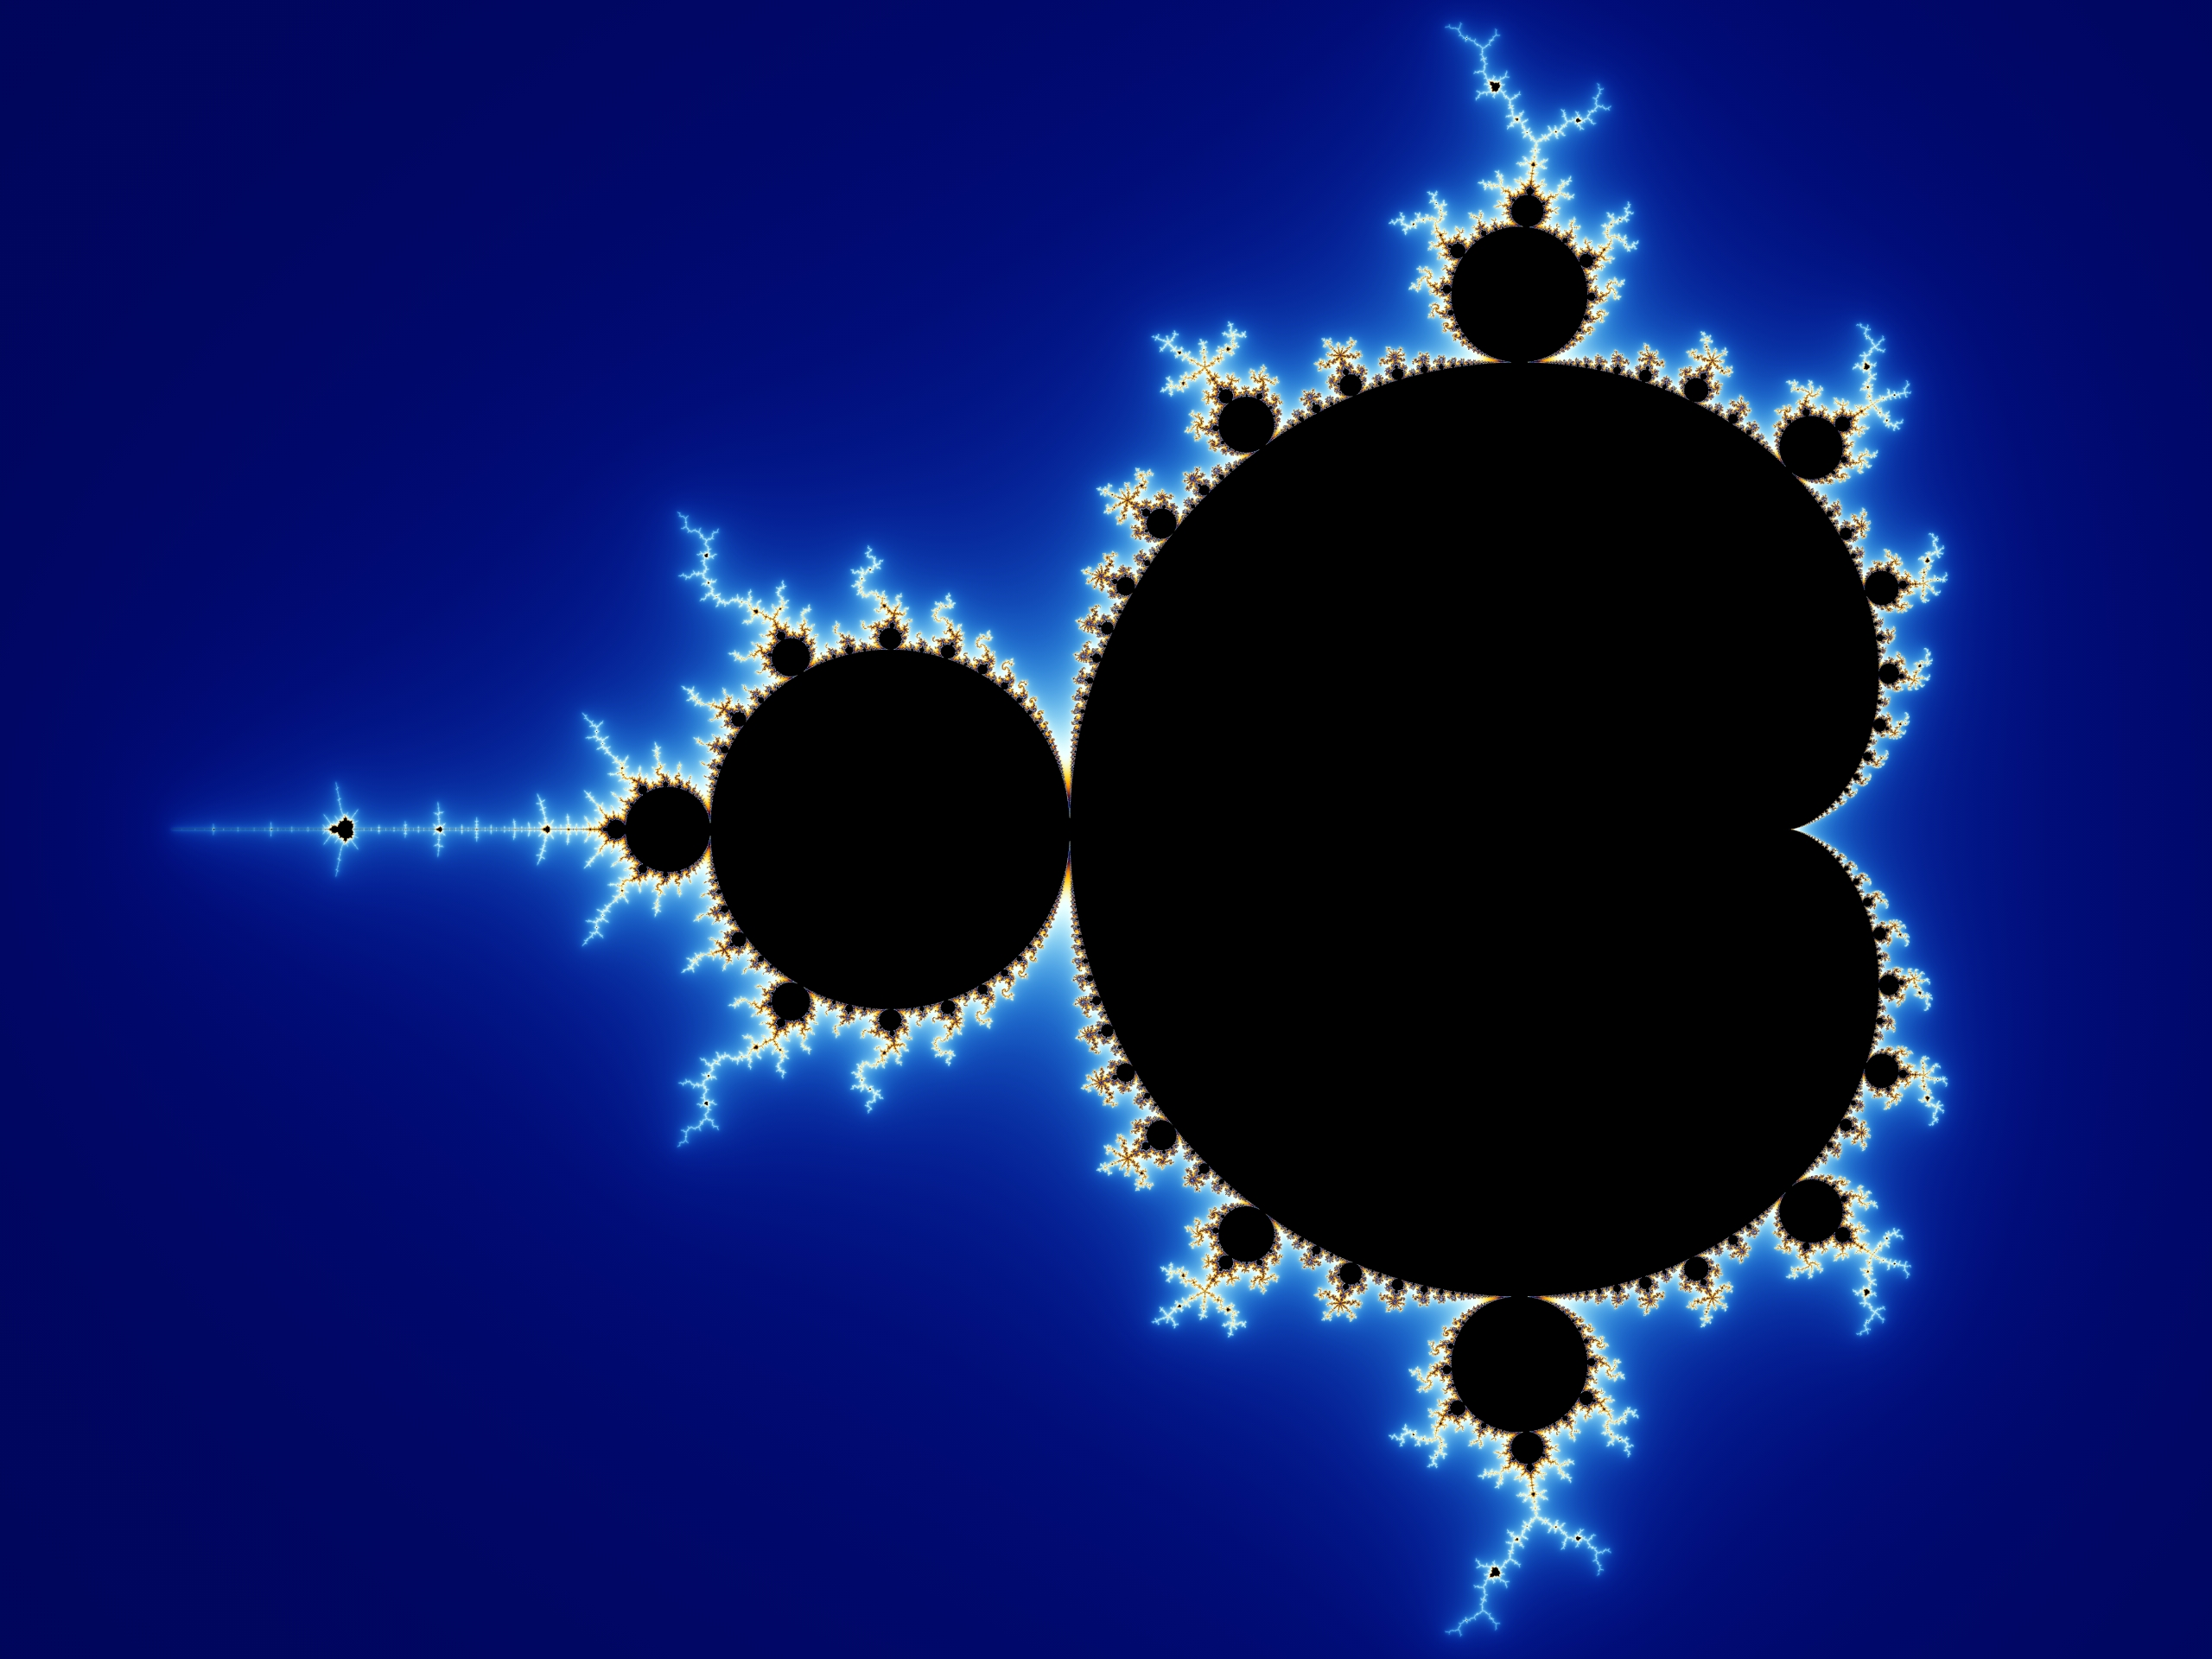
\includegraphics[height=1.0\linewidth,keepaspectratio]{figures/mandelbrot.jpg}}
          \end{figure}
      \end{column}
  \end{columns}
\end{frame}

\begin{frame}[plain]{\white{Program Synthesis}}
  % In practice, program synthesis is difficult, but effective.
  % Perhaps the best survey paper on the subject is by Sumit Gulwani et al, of Microsoft Research.
  % (pause)
  % My favorite example of program synthesis is a paper by Brendan Lake, Ruslan Salakhutdinov, and Joshua Tenenbaum.
  % In this paper, a powerful program representation is learned using a combination of bayesian inference and gradient methods.
  % The core takeaway from this paper is simply that *learned representation matters*
  
  % However, the core inspiration for this thesis is a paper by Google Brain,
  %   written by Real et al, and I'll go into more detail in a minute.
  \begin{columns}[T]
      \begin{column}{.5\linewidth}
          \vspace{1em}
          \emphasis{\cite{gulwani2017program}}
          \begin{itemize}
              \onslide<1->{\item Best Survey Paper}
          \end{itemize}
          \vspace{1em}
          \emphasis{\cite{lake2015human}}
          \begin{itemize}
              \onslide<2->{\item Bayesian Program Learning
              \item Representation matters}
          \end{itemize}
          \vspace{1em}
          \emphasis{\cite{real2020automl}}
          \begin{itemize}
              \onslide<3->{
              \item Tensor Program Learning 
              \item Core Thesis Inspiration}
          \end{itemize}
      \end{column}
      \begin{column}{.5\linewidth}
          \begin{figure}
              \vspace{-3.5em}
              \hspace*{1.3em}
              \rotatebox[origin=c]{-90}{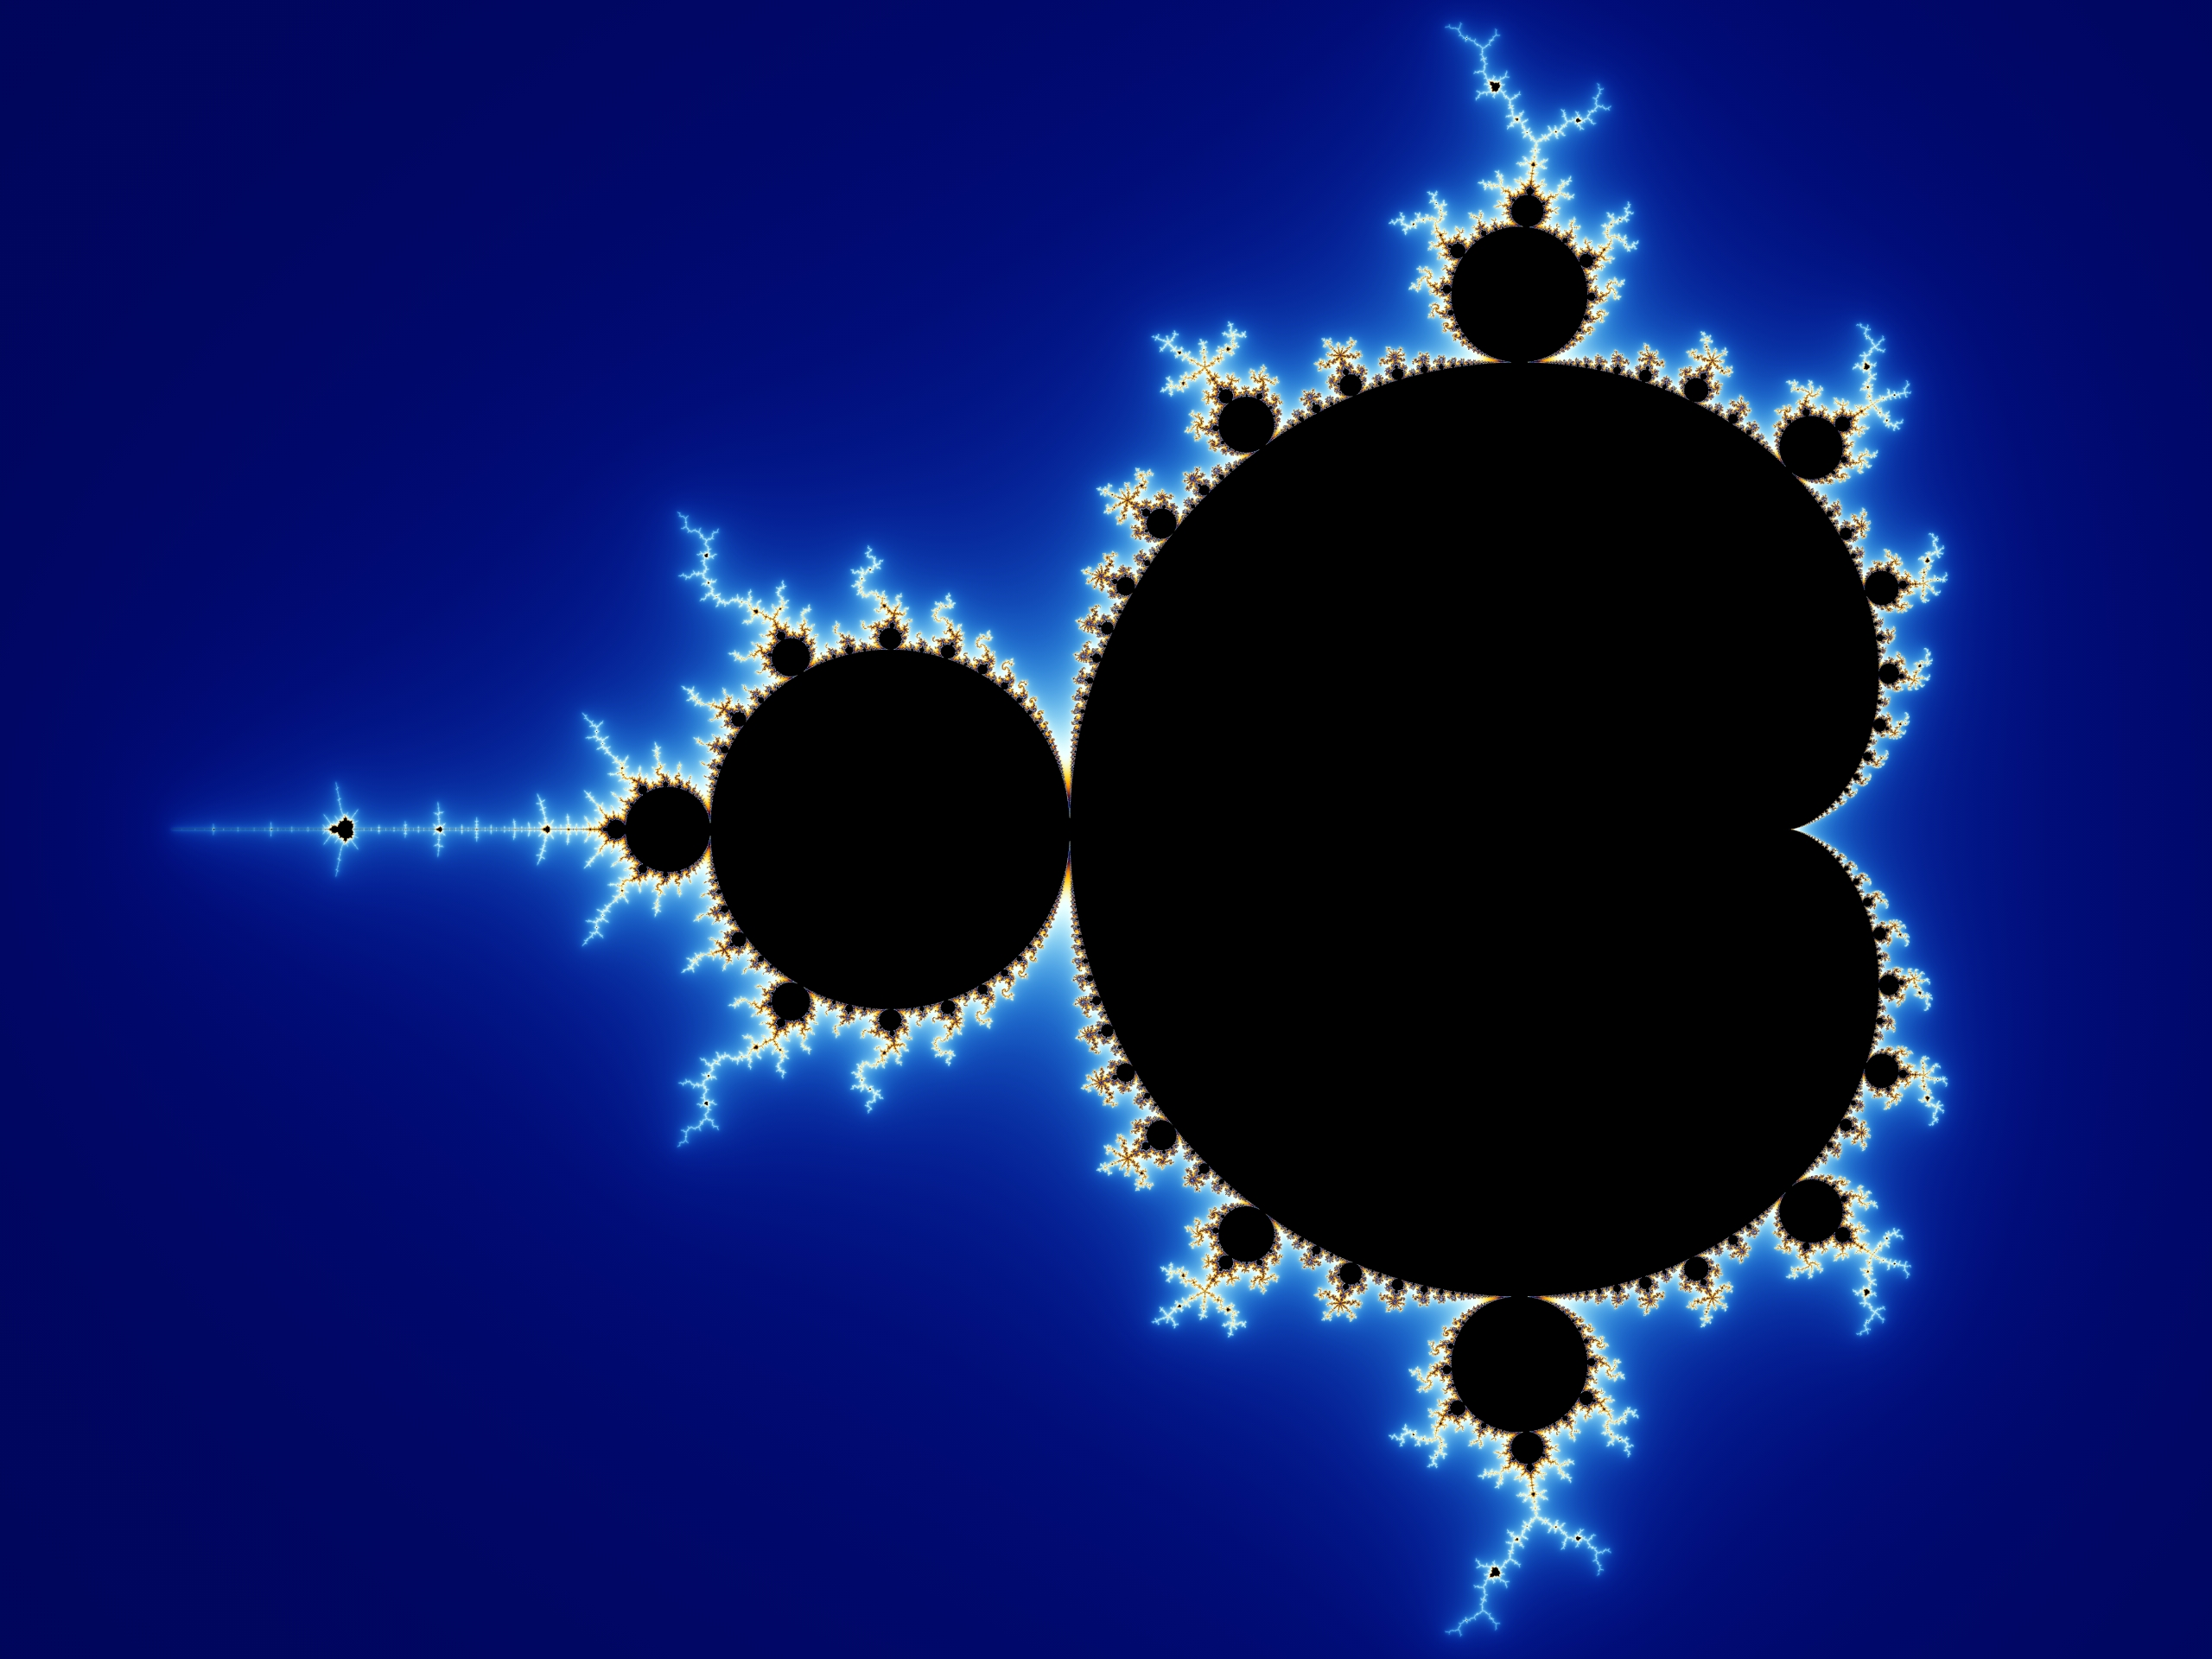
\includegraphics[height=1.0\linewidth,keepaspectratio]{figures/mandelbrot.jpg}}
          \end{figure}
      \end{column}
  \end{columns}
\end{frame}

\begin{frame}{Evolutionary/Genetic Algorithms}
  % The most relevant type of program synthesis is via Evolutionary algorithms
  % Using this is known as evolutionary programming.
  % 
  % In a nutshell, an evolutionary algorithm keeps a population
  %   of solutions, called members, which are being optimized for a particular goal.
  % Members are *encoded*, for instance as a vector of numbers or as computer programs.
  % If the encoding is a computer program, then the algorithm is doing evolutionary programming
  % 
  % Optimization is accomplished by *selecting* population members based on
  %   their *fitness* score, which is their performance on some goal.
  %
  % Mutation and crossover play an important role in this process.
  % Mutation refers to randomly changing a member of the population.
  % Crossover refers to combining two members of the population, which is
  %   an analogy to how human DNA is recombined.
  % 
  % On the right is a small evolutionary experiment.
  % Members are represented as points in space
  % Points are selected for based on fitness, which is the sum of their x and y components.
  % They are mutated by randomly regenerating a single coordinate.
  % The "After" figure shows three applications of selection.
  % As you can see, the average fitness of the population increases over time via this method.
  \begin{columns}[T]
      \begin{column}{.4\linewidth}
      \Huge \textit{\cb{Population Optimization}}
      \begin{vfilleditems}
          \item \Huge Selection
          \item \Huge Mutation
          \item \Huge Crossover
      \end{vfilleditems}
      \end{column}
      \begin{column}{.6\linewidth}
          \begin{figure}
              \centering
              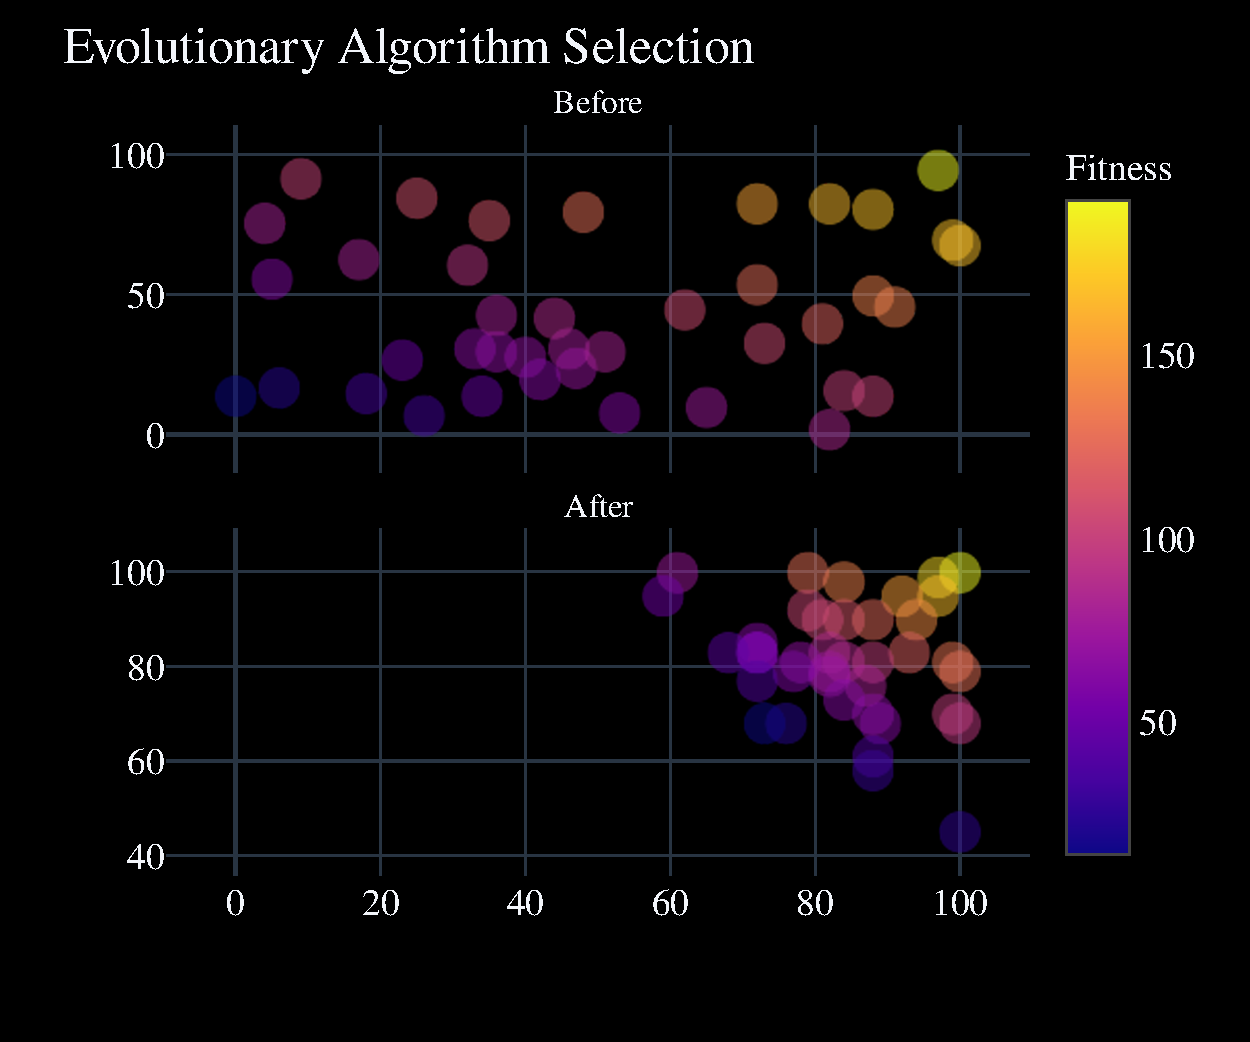
\includegraphics[width=0.95\linewidth, keepaspectratio]{figures/genetic_diagram.pdf}
          \end{figure}
      \end{column}
  \end{columns}
\end{frame}

\begin{frame}[plain]{}
  % First, consider this:
  % Many problems are actually program learning in disguise.
  % How can we classify these problems?
  \centering
  \vfill
  \red{\fontsize{40}{50}\selectfont Approach Classification}
  \vfill
\end{frame}

\begin{frame}{Approach Template Example}
  % Here, I've created a template which fits many important problems in computer science.

  % Now consider how a convolutional neural network might fit into this framework
  % First, there is an engineering problem, for example: Image Classification
  % Then, there is a choice of representation, for example: Neural Network Weights
  % Finally, there is a choice of optimization, for example: Gradient Methods
  % I'll use this template to explain previous work, as well as my own.
   \begin{columns}[T]
      \begin{tabular}{ll}
           {\Huge Problem}        &  \onslide<2->{\cb{\Huge Image Classification}}  \\
           &\\
           {\Huge Representation} & \onslide<3->{\cc{\Huge Network Weights}} \\
           &\\
           {\Huge Optimization}   & \onslide<4->{\ce{\Huge Gradient Methods}} \\
      \end{tabular}
  \end{columns}
\end{frame}


\begin{frame}[plain]{}
  % That was an example of machine learning
  % Now, consider the word Meta, as in Meta-learning.
  % Reffering to itself, or to the conventions of its genre; *Self-Referential*
  \centering
  \vfill
  \red{\fontsize{40}{50}\selectfont "Meta"}
  \vfill
  \Large Referring to itself or to the conventions of its genre; \cc{self-referential} \gr{(Wikipedia Definition)}
\end{frame}

\begin{frame}{AutoML-Zero: Evolving Machine Learning Algorithms From Scratch \white{\cite{real2020automl}}}
  % AutoML-Zero, by Real et al, is an example of Meta-Learning.
  % Instead of learning a task directly, it attempts to learn how to do machine learning.
  % Also, it makes very few assumptions, and attempts to start from scratch.
  %
  % Consider how this fits into the approach template:
  %   The subtask is image-classification on CIFAR-10, which is conventionally done
  %     with a convolutional neural network.
  %   To meta-learn how to do classification, this paper represents neural networks via a
  %     **Tensor Register Machine**. This is their program representation.
  %   This program representation is optimized via Regularized Evolution, which is 
  %     an evolutionary algorithm.
    \begin{vfilleditems}
        \item \cb{\Huge Learns ML practices on CIFAR-10}
        \vspace{0.7em}
        \item \cc{\Huge Tensor register machine}
        \vspace{0.7em}
        \item \ce{\Huge Regularized Evolution}
    \end{vfilleditems}
\end{frame}

\begin{frame}{Regularized Evolution}
  % Regularized Evolution is a fast, stable method for population optimization.
  % Crucially, Regularized Evolution uses *aging*.
  % The population is represented as a queue, with young members at the start and old members at the end.
  % Every iteration, Reg. Ev. samples a subset of the population.
  % The best member is selected from this sample.
  % Then, the oldest member of the population is discarded.
    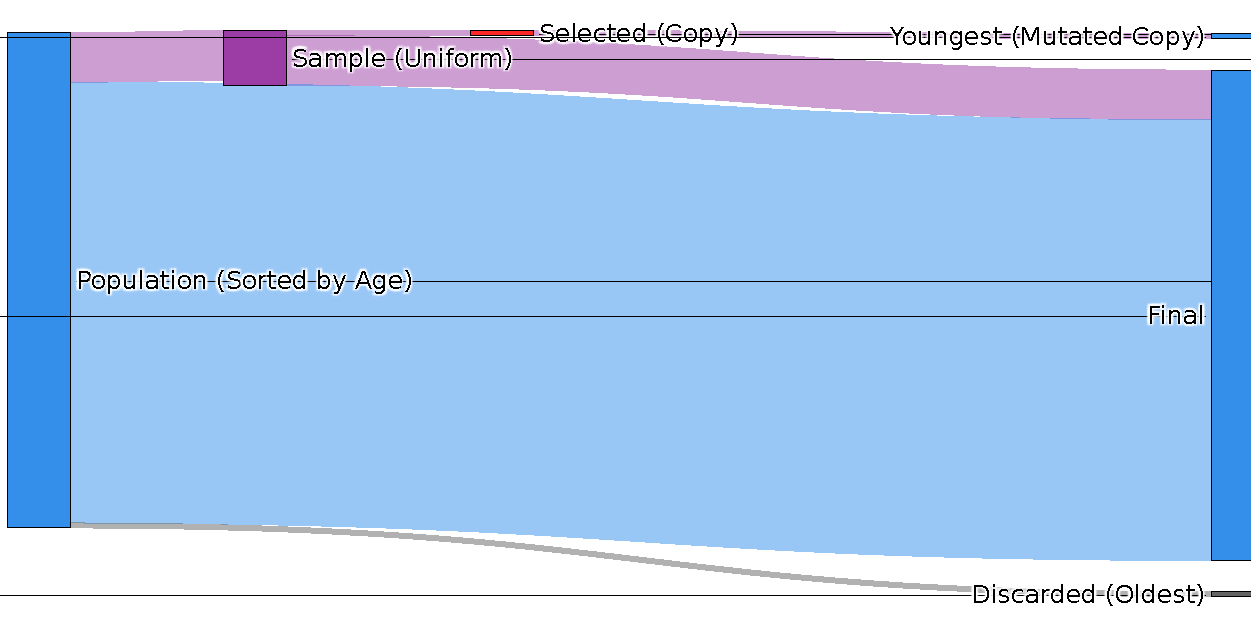
\includegraphics[width=0.95\linewidth, keepaspectratio]{figures/regev.pdf}
\end{frame}

\begin{frame}[plain]{AutoML-Zero \white{\cite{real2020automl}}}
  % Here is the central result of the AutoML-Zero paper.
  % The y-axis shows the accuracy of the best-learned image classifier.
  % The x-axis shows the number of potential learning algorithms that have been evaluated.
  % Note that the x-axis is logarithmic.
  % Because of this, Google considers 10 billion algorithms before they reach the first promising one
  % Then, between considering 10 billion and one trillion algorithms,
  %   the best-found image classification model gradually improves.
  % Improvements come from the algorithm finding various machine learning practices.
  % First, a linear model is learned.
  % Then, stochastic gradient descent is learned.
  % Eventually, a competitive modern classifier is evolved.
    \begin{figure}
        \centering
        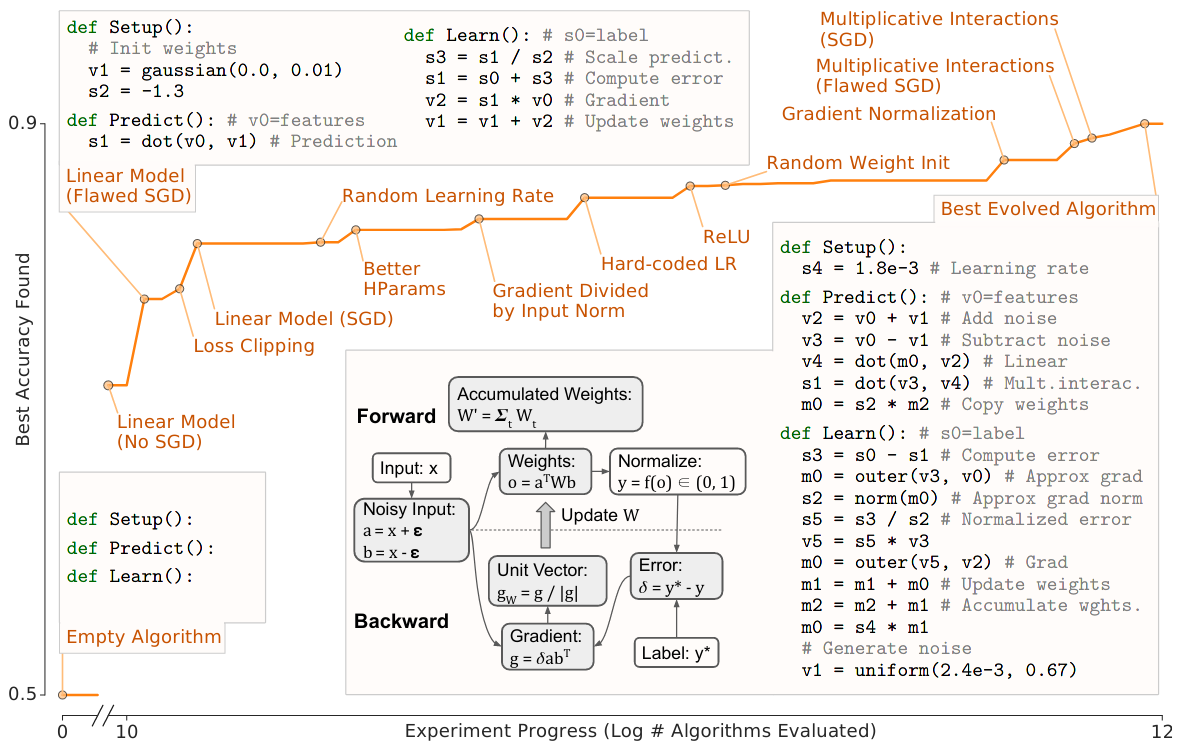
\includegraphics[scale=0.37]{figures/automl_zero_main_fig.png}
    \end{figure}
\end{frame}

\begin{frame}{Environment Learning for Path-Planning}
    \begin{vfilleditems}
        \item \cb{\Huge Path Planning}
        \vspace{0.7em}
        \item \cc{\Huge Python Programs}
        \vspace{0.7em}
        \item \ce{\Huge Pareto Evolution}
    \end{vfilleditems}
\end{frame}

\begin{frame}{{\color{pureminimalistic@text@white} Multiple Objectives}}
  % Path Planning has multiple objectives.
  %   In the most basic form, these are the number of nodes considered, and the length of the eventual path.
  % However, other metrics, like exploration, can be relevant, but the main point 
  %   is that there are multiple objectives.
  % On the right is a plot, where each point is a computer program.
  % The x-axis is the number of nodes considered, 
  %   and the y-axis is the path length.
  % Each point is labeled with its *age*, or the iteration that it was found at.
  
  % The total array of points forms an interesting distribution, where no single point is perfect, and instead algorithms make trade-offs with one-another.
  \begin{columns}[T]
      \begin{column}{.4\linewidth}
          \emphasis{Nodes}
          \vspace{1em}
          \newline
          \emphasis{Path Length}
          \vspace{1em}
          \newline
          \emphasis{Exploration}
          \newline
          \vspace*{1em}
          \begin{center}
          \emphasis{\ldots }
          \end{center}
      \end{column}
      \begin{column}{.6\linewidth}
      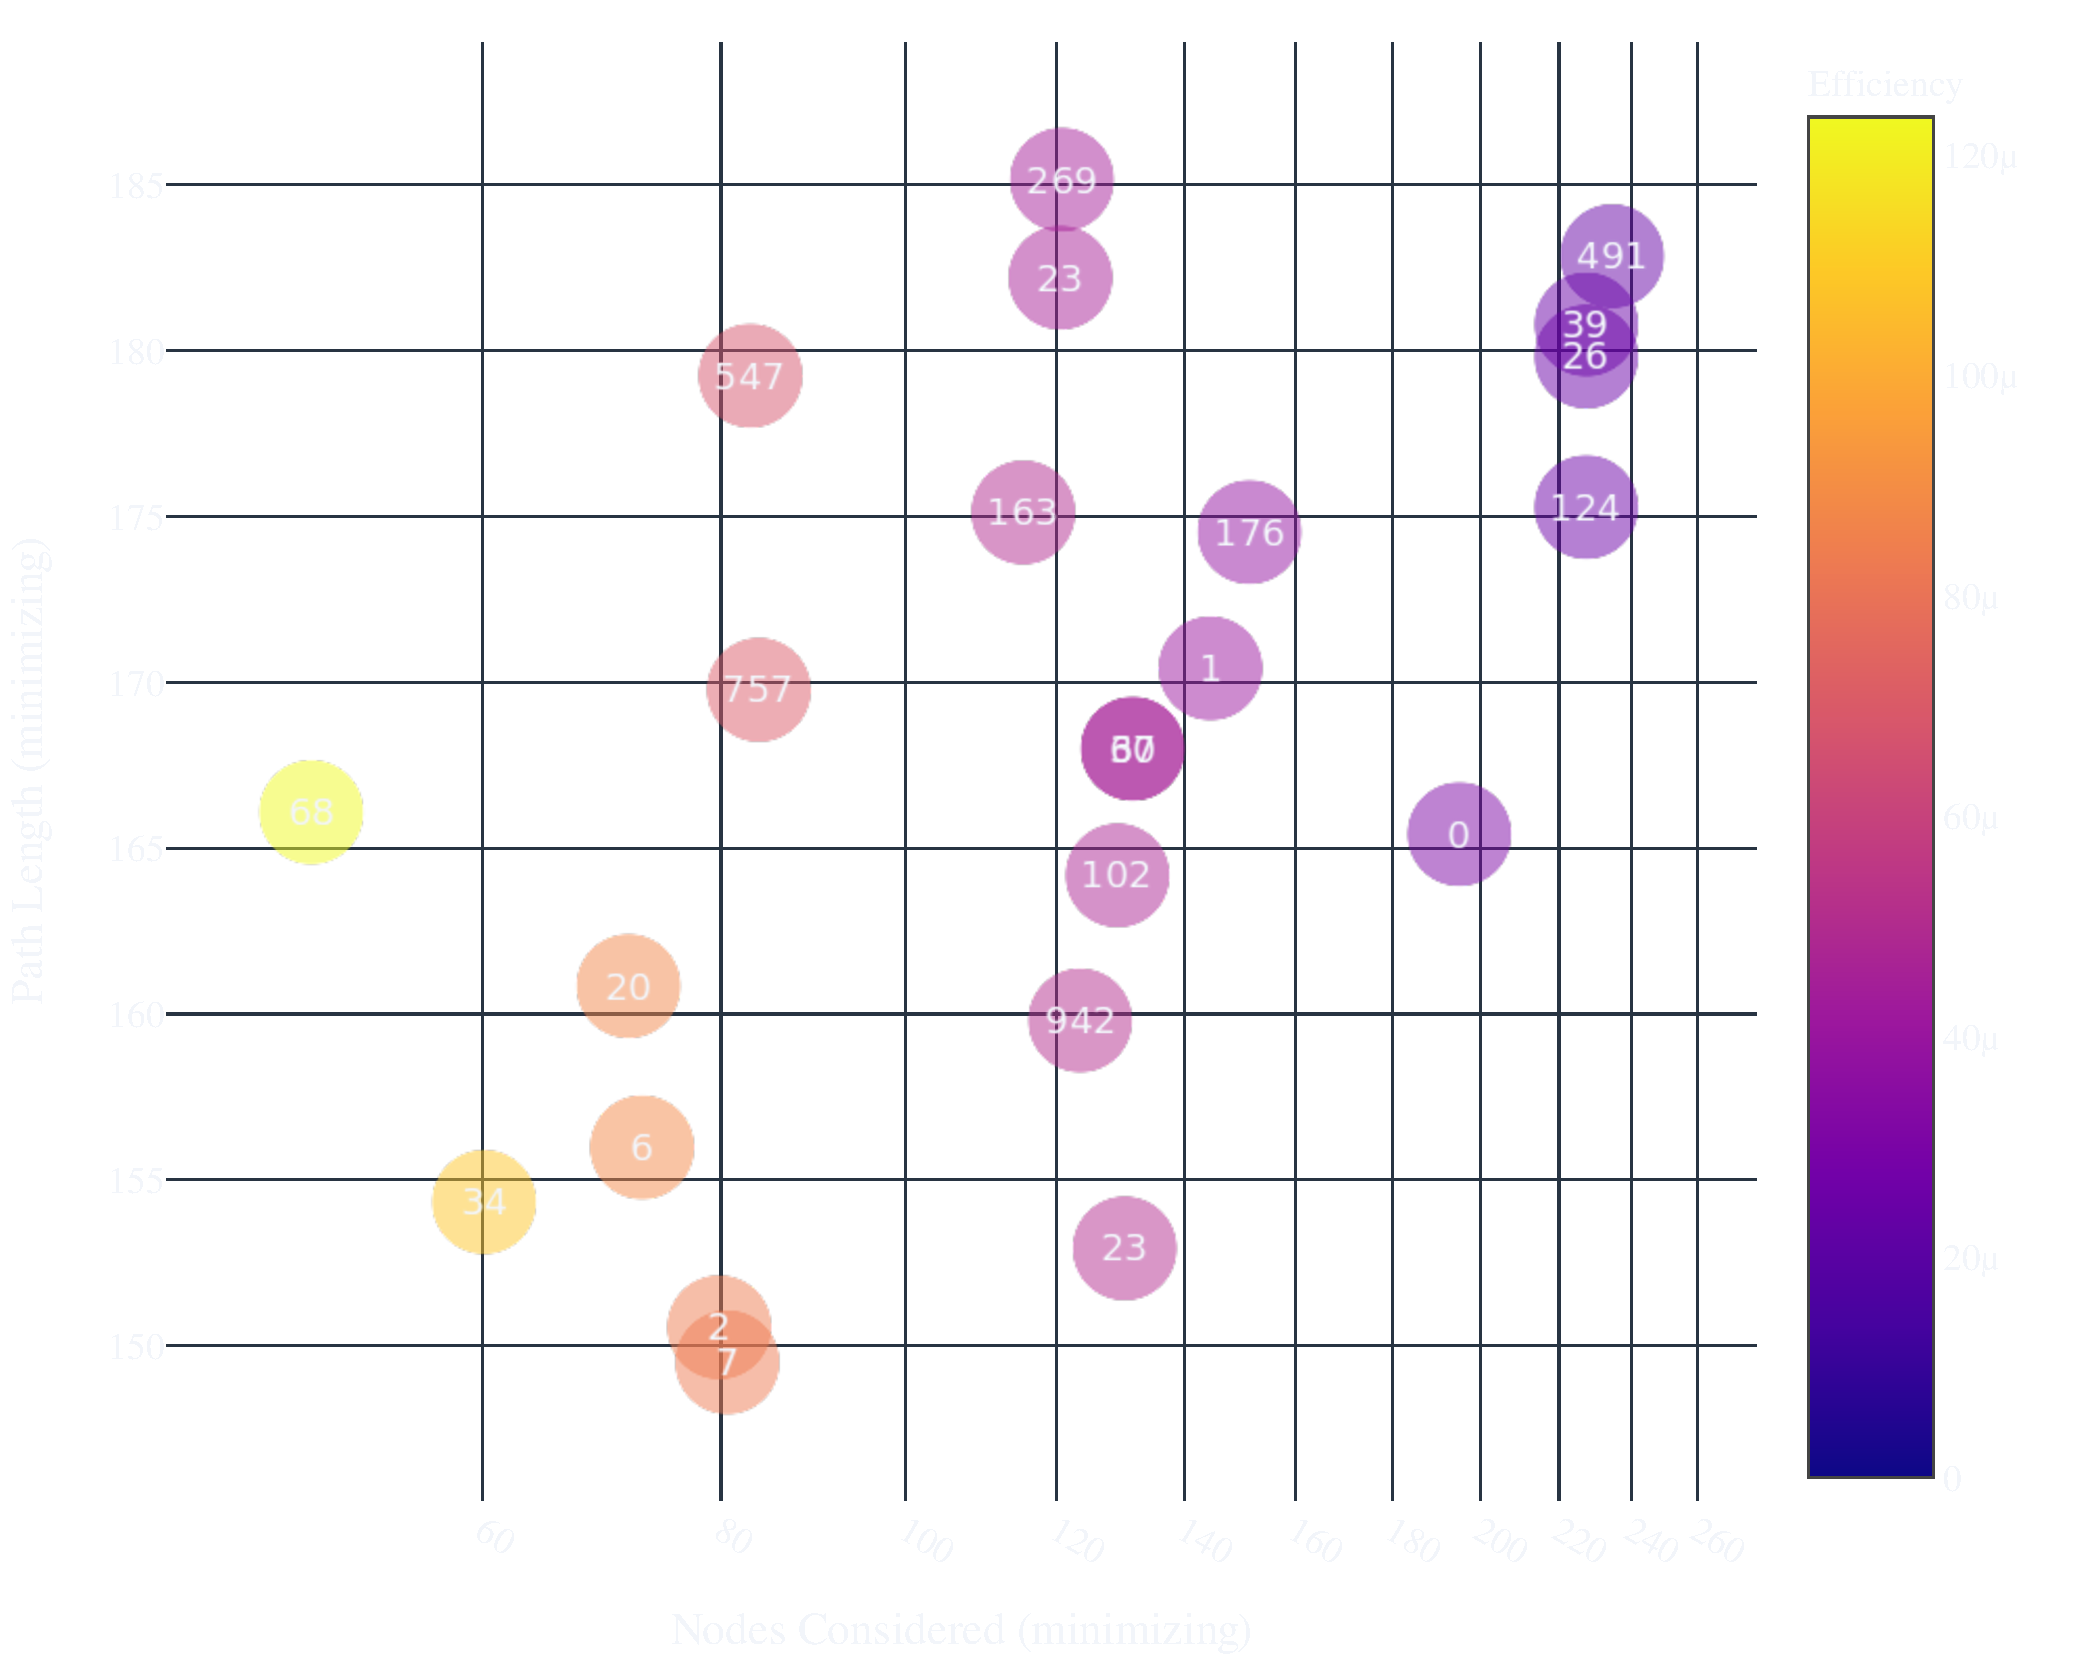
\includegraphics[width=0.9\linewidth, keepaspectratio]{figures/total_overview.pdf}
      \end{column}
  \end{columns}
\end{frame}

\begin{frame}{Pareto Fronts}
  % These trade-offs are defined in the form of *Pareto Fronts*.
  
  % First, each algorithm is evaluated by a _fitness_,
  %   which is a vector because there are multiple objectives.
  % Pareto equivalence is defined by an ordering on fitness vectors.
  % If one fitness vector is not strictly superior in all elements,
  %   Then it is said to be Pareto-equivalent to another.
  % For example, v1 and v2 are Pareto-equivalent because while
  %   v1 has the shortest path, v2 considers fewer nodes.
  % In the same way, v3 is also pareto-equivalent
  % Because these three members are pareto-equivalent, they are placed in the first pareto front.
  % However, v4 is not, because v1 strictly outperforms it on both metrics.
  
  % These fronts are shown via the curves in this figure. 
  \begin{columns}[T]
      \begin{column}{.4\linewidth}
          \begin{vfilleditems}
              \item {\Large Vectorized Fitness}
              \begin{tabular}{ll}
              &  \\
              & {\Large $v_i = \{\red{nodes, path}\}$} \\
              &  \\
              \end{tabular}
              \item {\Large Pareto Equivalence}
              \begin{tabular}{ll}
              &  \\
              & {\Large $v_1 = \{\cc{80, 151}\}$} \\
              & {\Large $v_2 = \{\cc{60, 155}\}$} \\
              & {\Large $v_3 = \{\cc{50, 165}\}$} \\
              &  \\
              & {\Large $v_4 = \{\cb{130, 153}\}$} \\
              \end{tabular}
          \end{vfilleditems}
      \end{column}
      \begin{column}{.6\linewidth}
      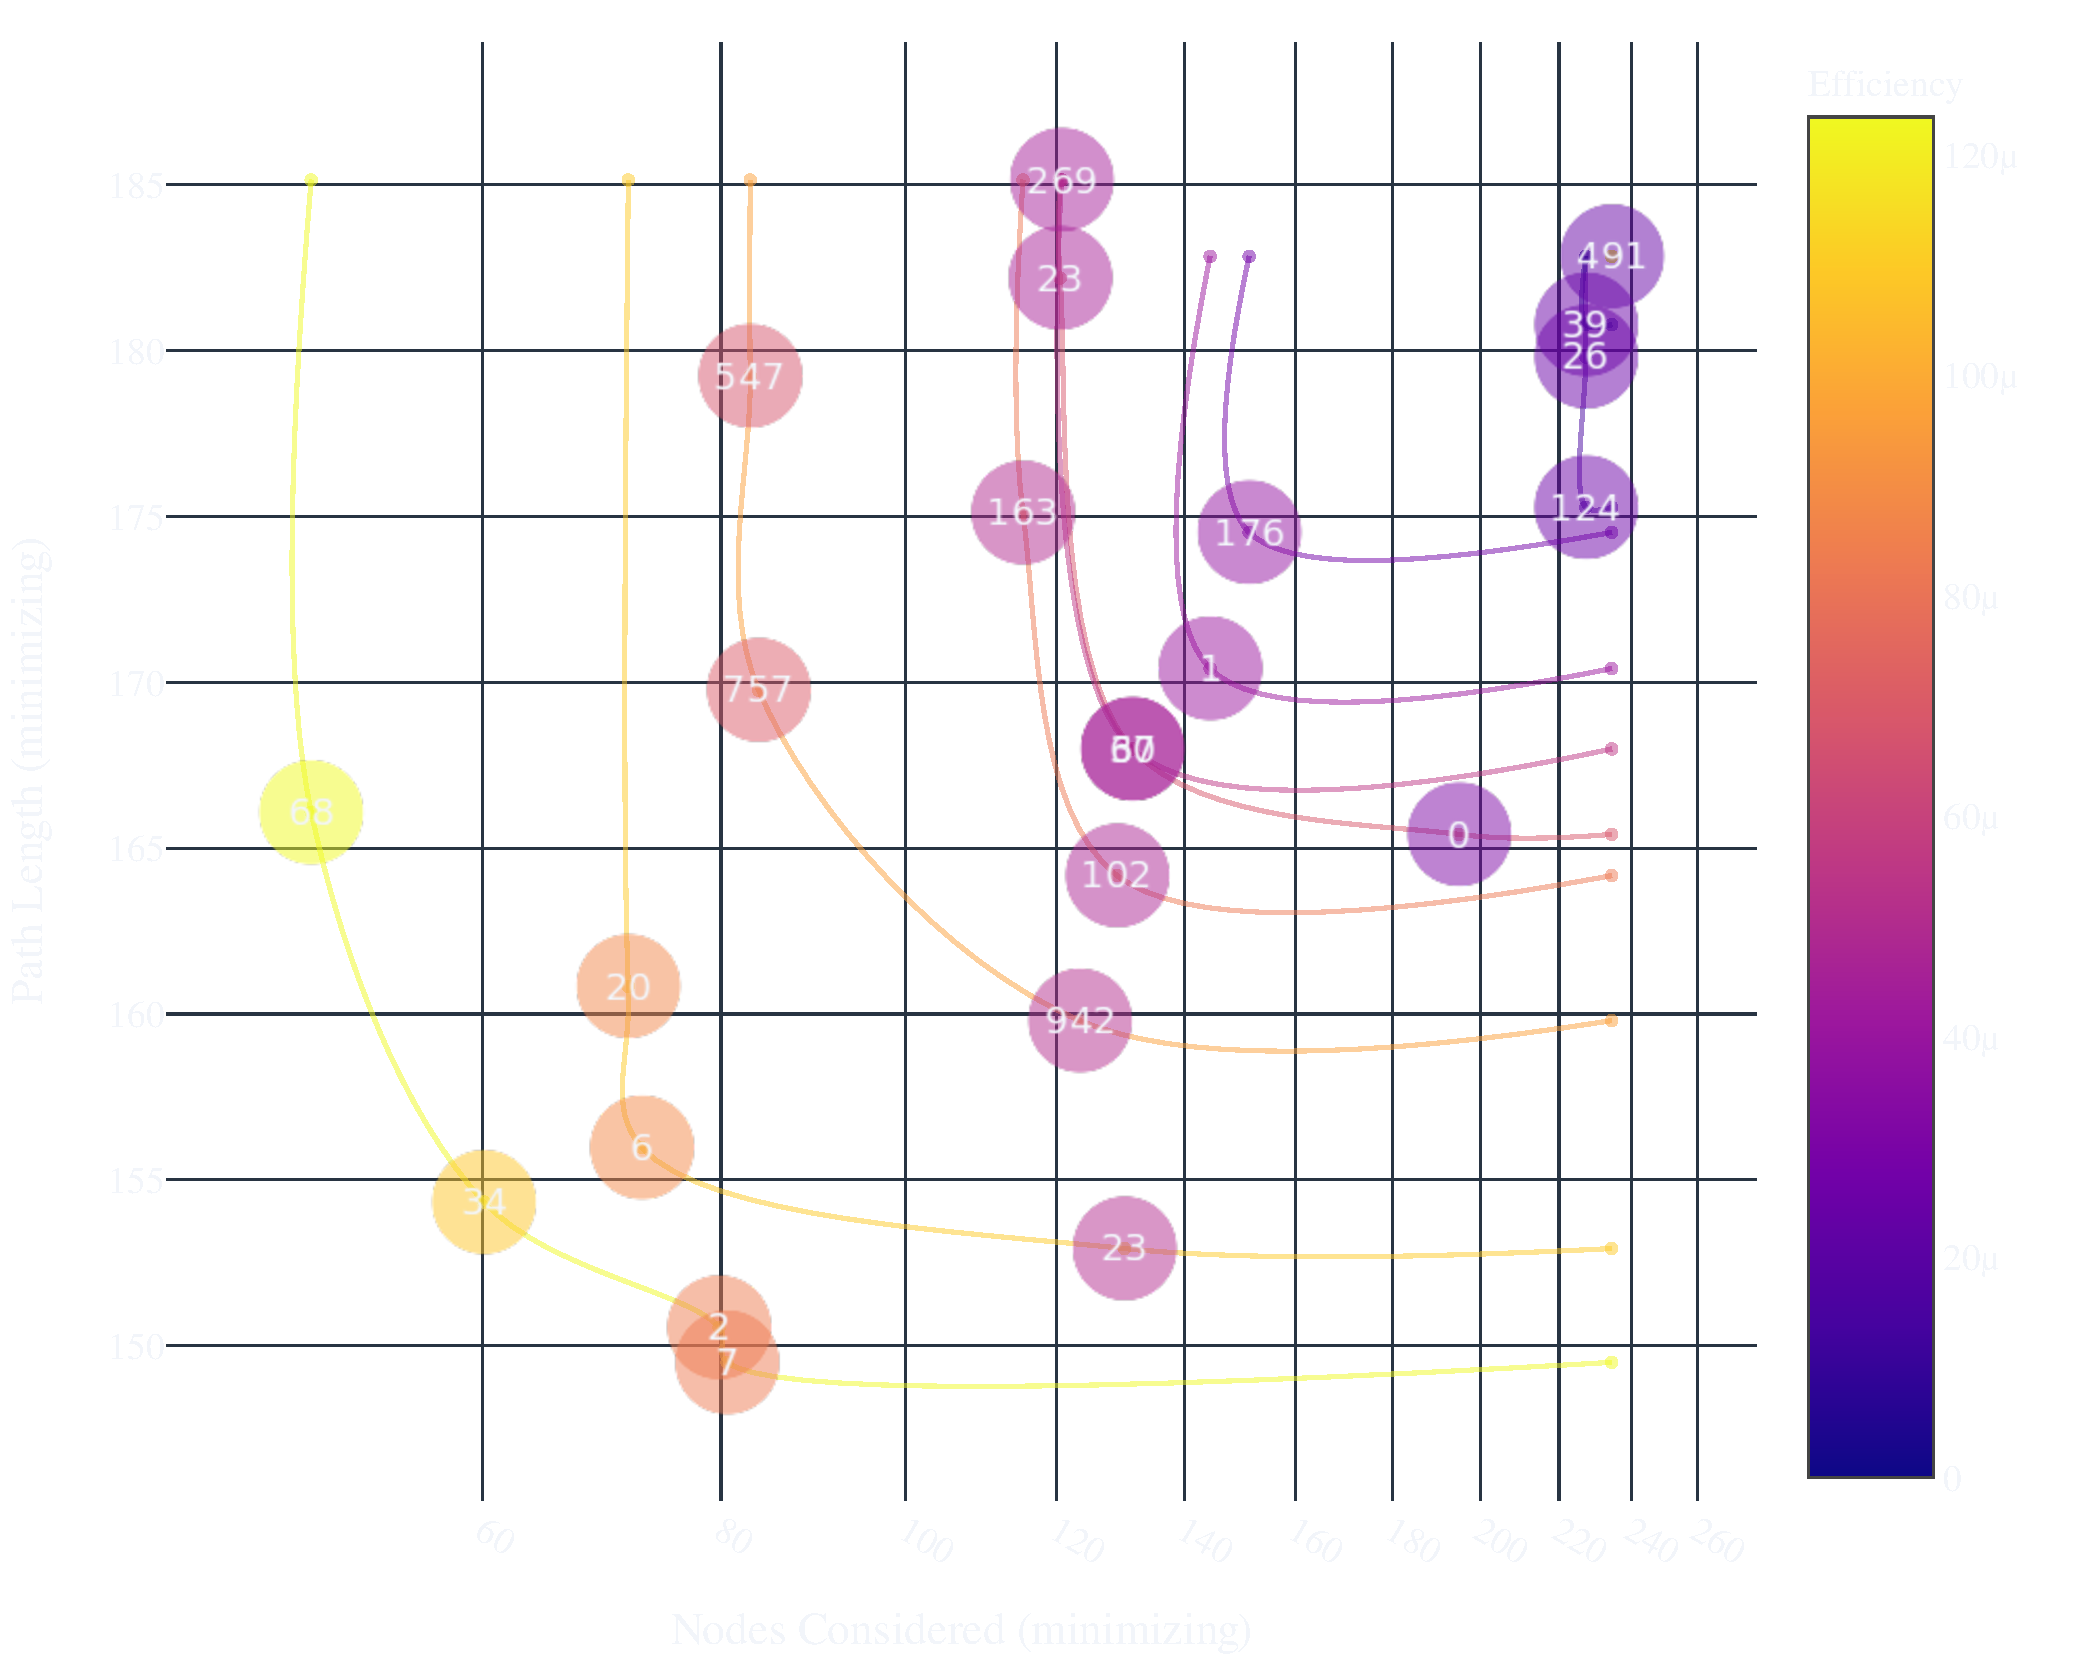
\includegraphics[width=0.9\linewidth, keepaspectratio]{figures/total_pareto_overview.pdf}
      \end{column}
  \end{columns}
\end{frame}

\begin{frame}{Evolvable Python Programs}
  \begin{columns}[T]
      \begin{column}{.5\linewidth}
      \begin{lstlisting}[language=Python]
          def build(K=1000):
              tree = Tree()
              for k in range(K):
                  rrt_extend(tree)
              return tree
          import numpy as np
      \end{lstlisting}
      Representation
      \end{column}
      \begin{column}{.5\linewidth}
      Mutation
      \end{column}
  \end{columns}
\end{frame}

\begin{frame}{Pareto Evolution}
    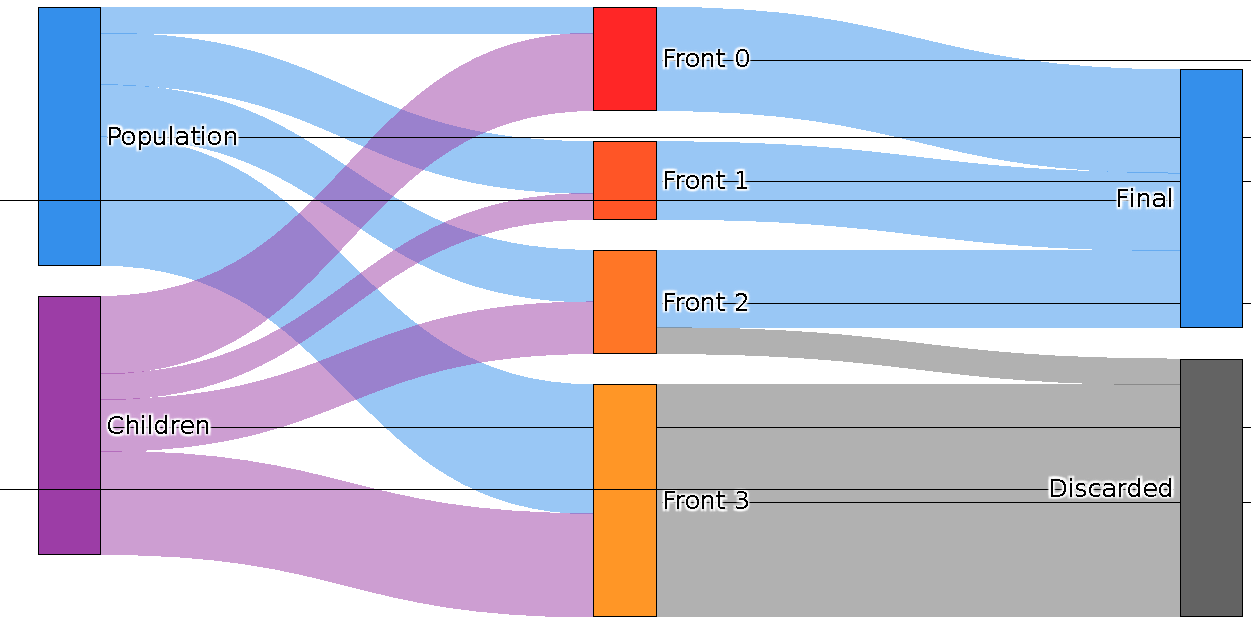
\includegraphics[width=1.0\linewidth, keepaspectratio]{figures/paretoev.pdf}
\end{frame}


\begin{frame}{}
  \begin{columns}[T]
      \begin{column}{.5\linewidth}
        \emphasis{Pareto Ev.} {\color{grey} \Medium (NSGA2)}
        \begin{itemize}
            \item Multi-objective
            \item Bandwidth: {\Large $\cc{n}$}
        \end{itemize}
        \vspace{1em}
        \begin{tabular}{ll}
        &\onslide<2->{{\Large $O(\ca{g} * \cb{m} * \cc{n}^\red{2})$}}          \\
        &\onslide<3->{{\Large $O(\cb{m} * \cc{n})$} {\color{grey} per change}} \\
        &\onslide<4->{{\Large $O(\cb{m} * \cd{p})$} {\color{grey} if sampled}} \\
        \end{tabular}
      \end{column}
      \begin{column}{.5\linewidth}
        \emphasis{Regularized Ev.}
        \begin{itemize}
            \item Single-objective
            \item Bandwidth: {\Large $\cc{1}$}
        \end{itemize}
        \vspace{1em}
        \begin{tabular}{ll}
        &\onslide<2->{{\Large $O(\ca{g} * \cd{p})$}}\\
        &\onslide<3->{{\Large $O(\cd{p})$} {\color{grey} per change}}\\
        &\onslide<4->{{\Large $O(\cd{p})$} {\color{grey} (sampled)}} \\
        \end{tabular}
      \end{column}
  \end{columns}
  \begin{center}
  \Large
      \onslide<2->{
      \begin{tabular}{ll}
        Where & \ca{$g = $ generations} \\
              & \cb{$m = $ objectives}  \\
              & \cc{$n = $ total population size}\\
              & \cd{$p = $ sample size}\\
     \end{tabular}
     }
  \end{center}
\end{frame}

\begin{frame}{Population Dynamics: Starcraft Engima}
  % Here is an example of the population dynamics of an optimization run.
    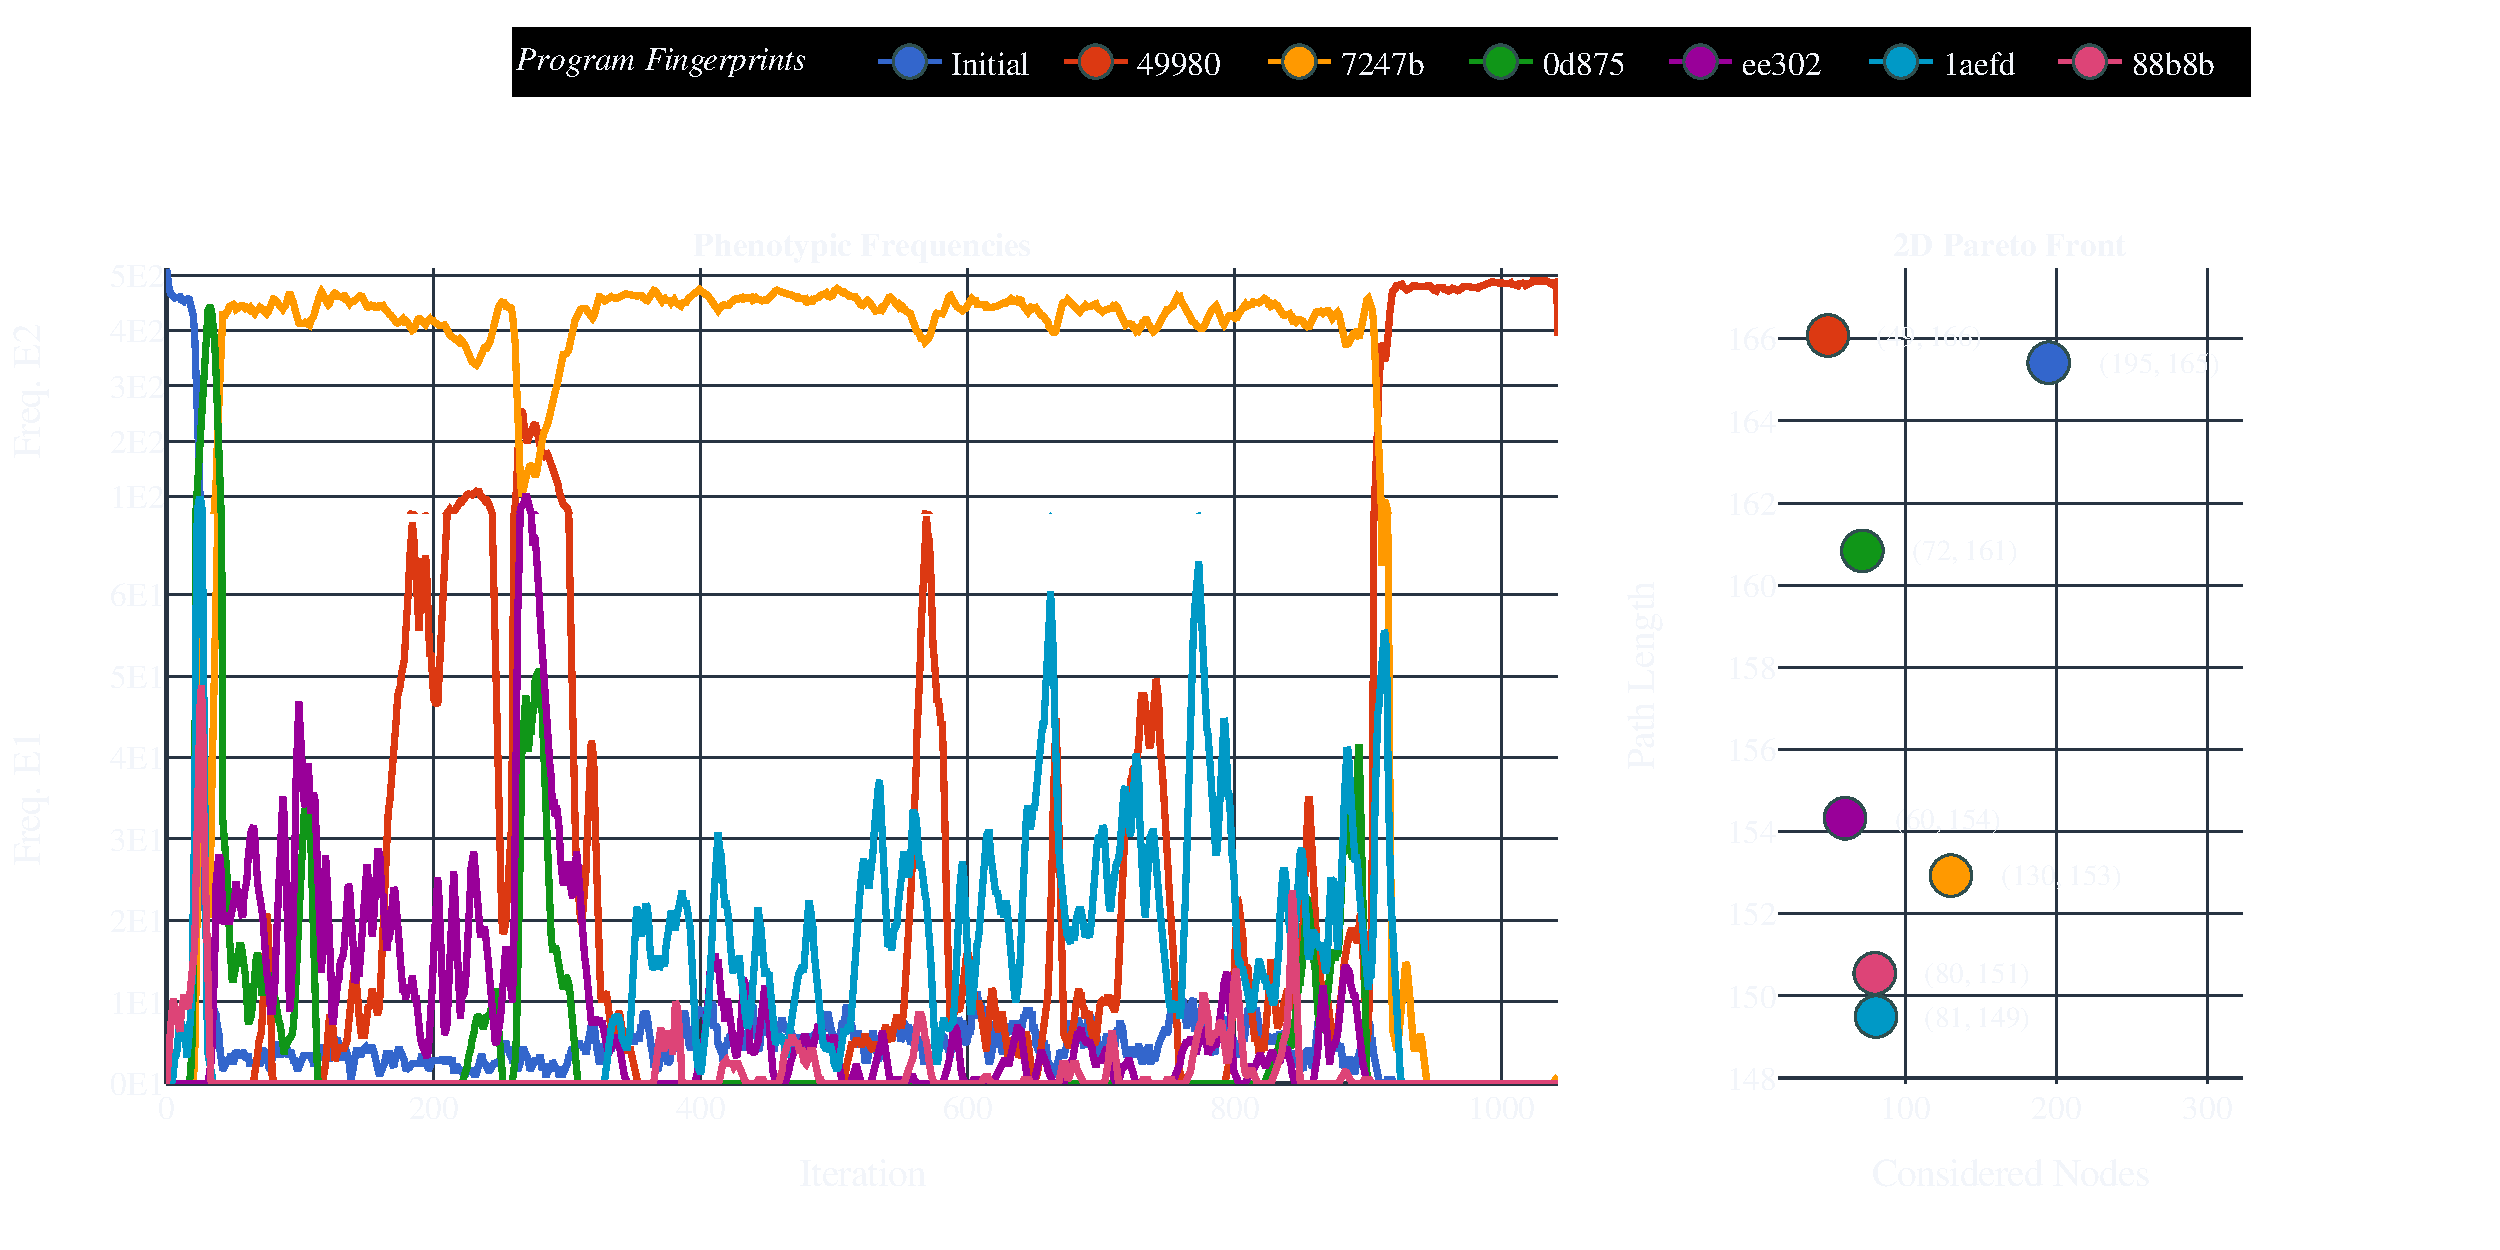
\includegraphics[width=1.0\linewidth, keepaspectratio]{figures/pheno.pdf}
\end{frame}

\begin{frame}{Specialization Results}
    % Here are the results of specializing algorithms to particular maps.
    % This experiment looked at five different scenarios:
    %   Milan, Italy, which is a relatively cluttered map
    %   A blank map,  which is intentionally open and easy to specialize to.
    %   A validation map, which is highly cluttered and tight.
    % The main experiment used three starcraft maps: Enigma, Turbo, and Entanglement.
    % More starcraft maps have been used in other experiments
    
    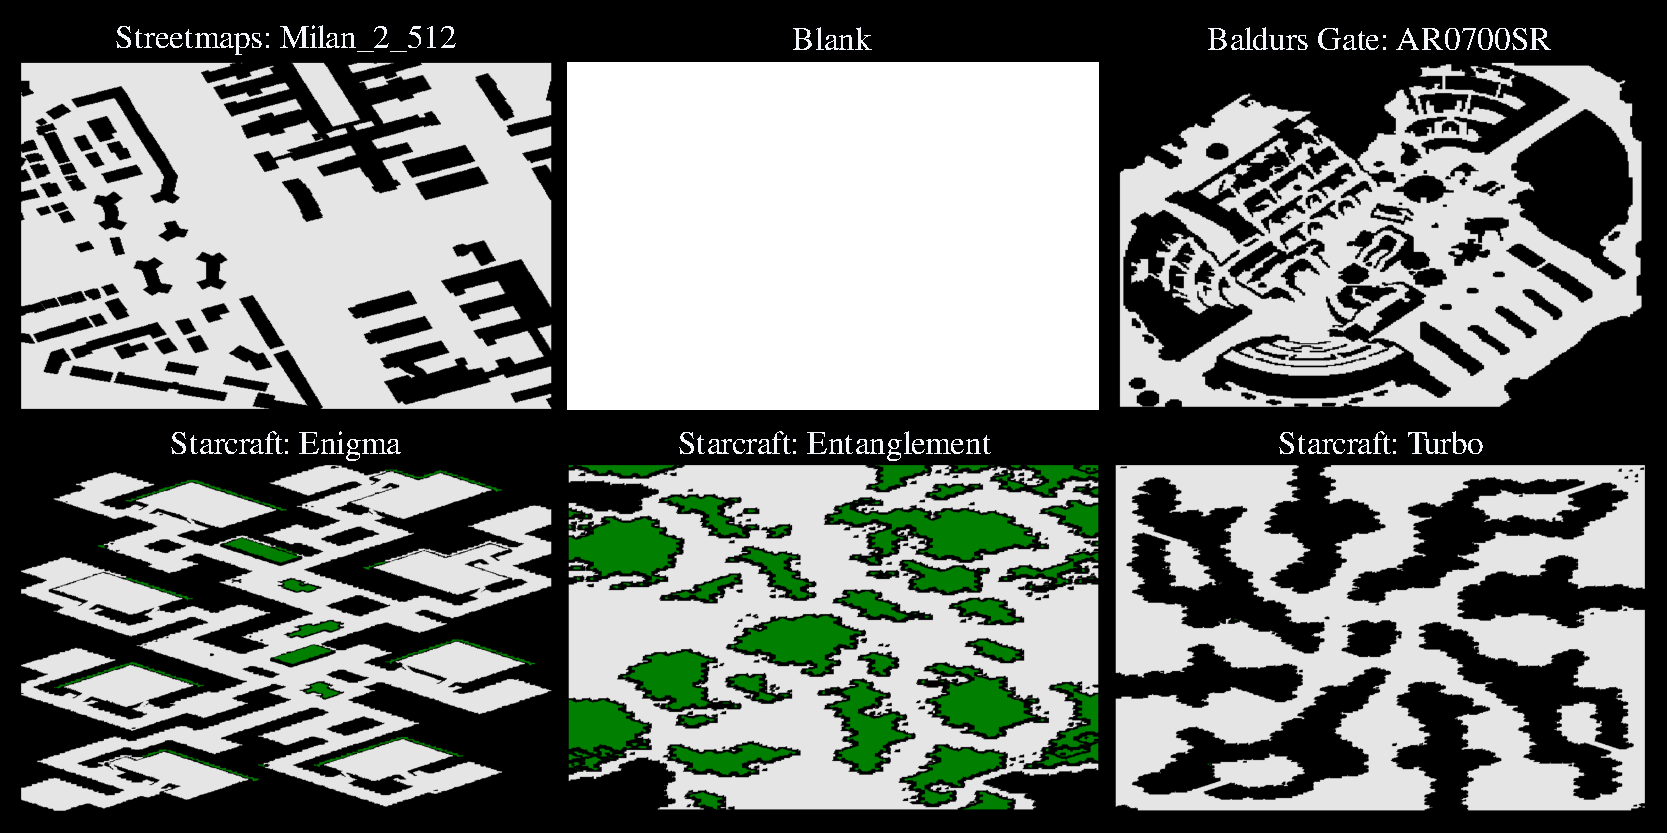
\includegraphics[width=1.0\linewidth, keepaspectratio]{figures/show_maps_exp.pdf}
\end{frame}

\begin{frame}{Specialization Results}
    % This is an overview of all specialized algorithms.
    % Simply note their different behaviors.
    % Now, I'll go through them in depth.
    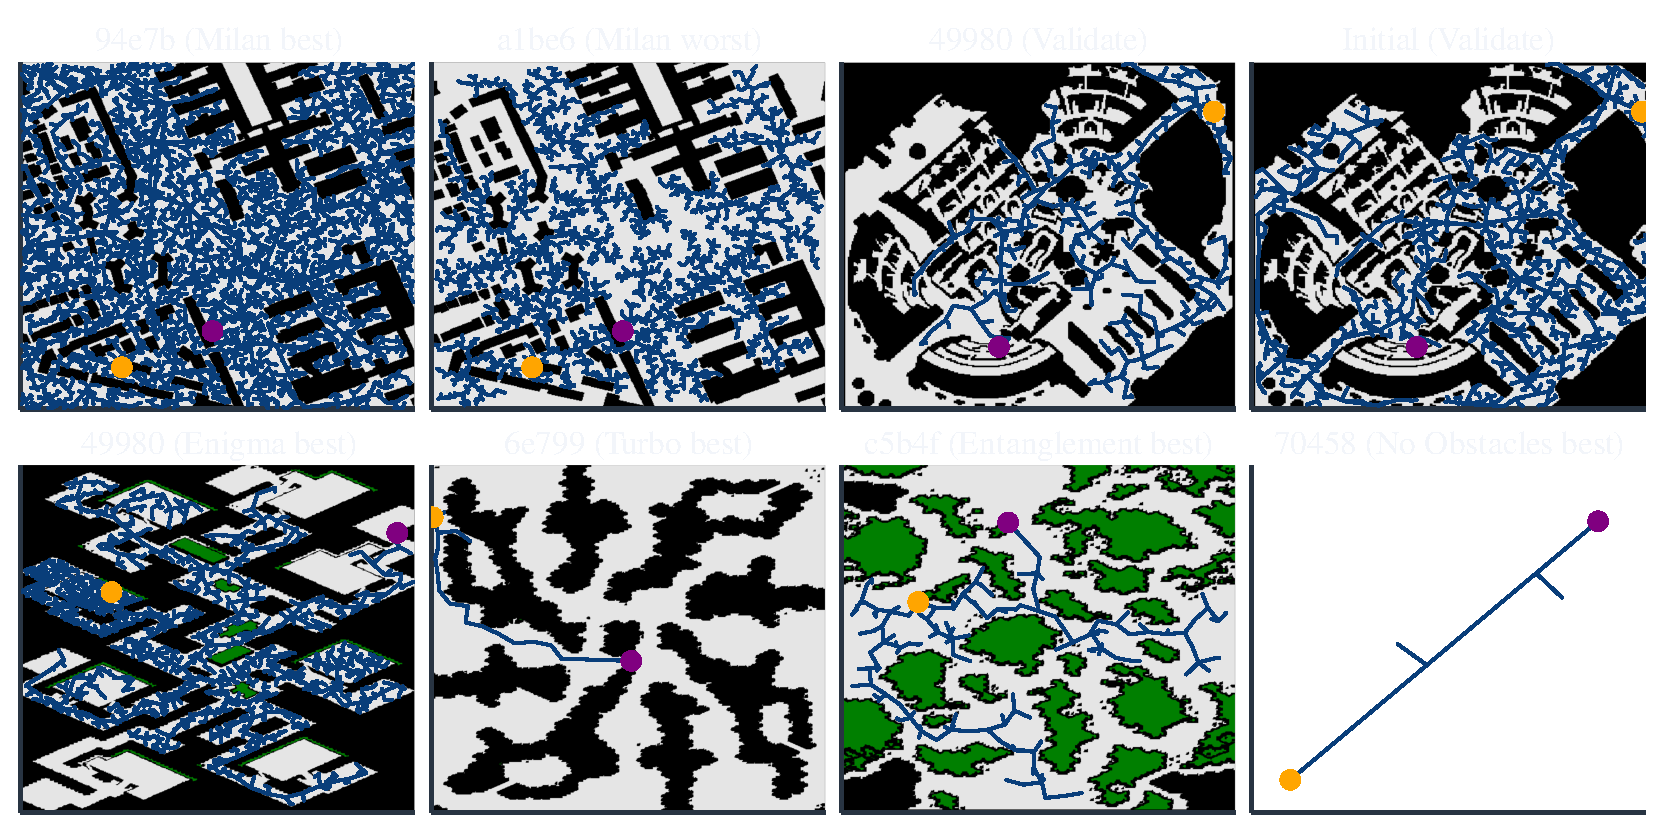
\includegraphics[width=1.0\linewidth, keepaspectratio]{figures/learned.pdf}
\end{frame}

\begin{frame}{Milan Best/Worst}
    % On the Milan map, the best planner learned *NOT* to bias towards the goal,
    % And instead learned to take very large steps.
    % The worst Milan planner was one which takes very small steps, but eventually covers the search space very evenly.
    
    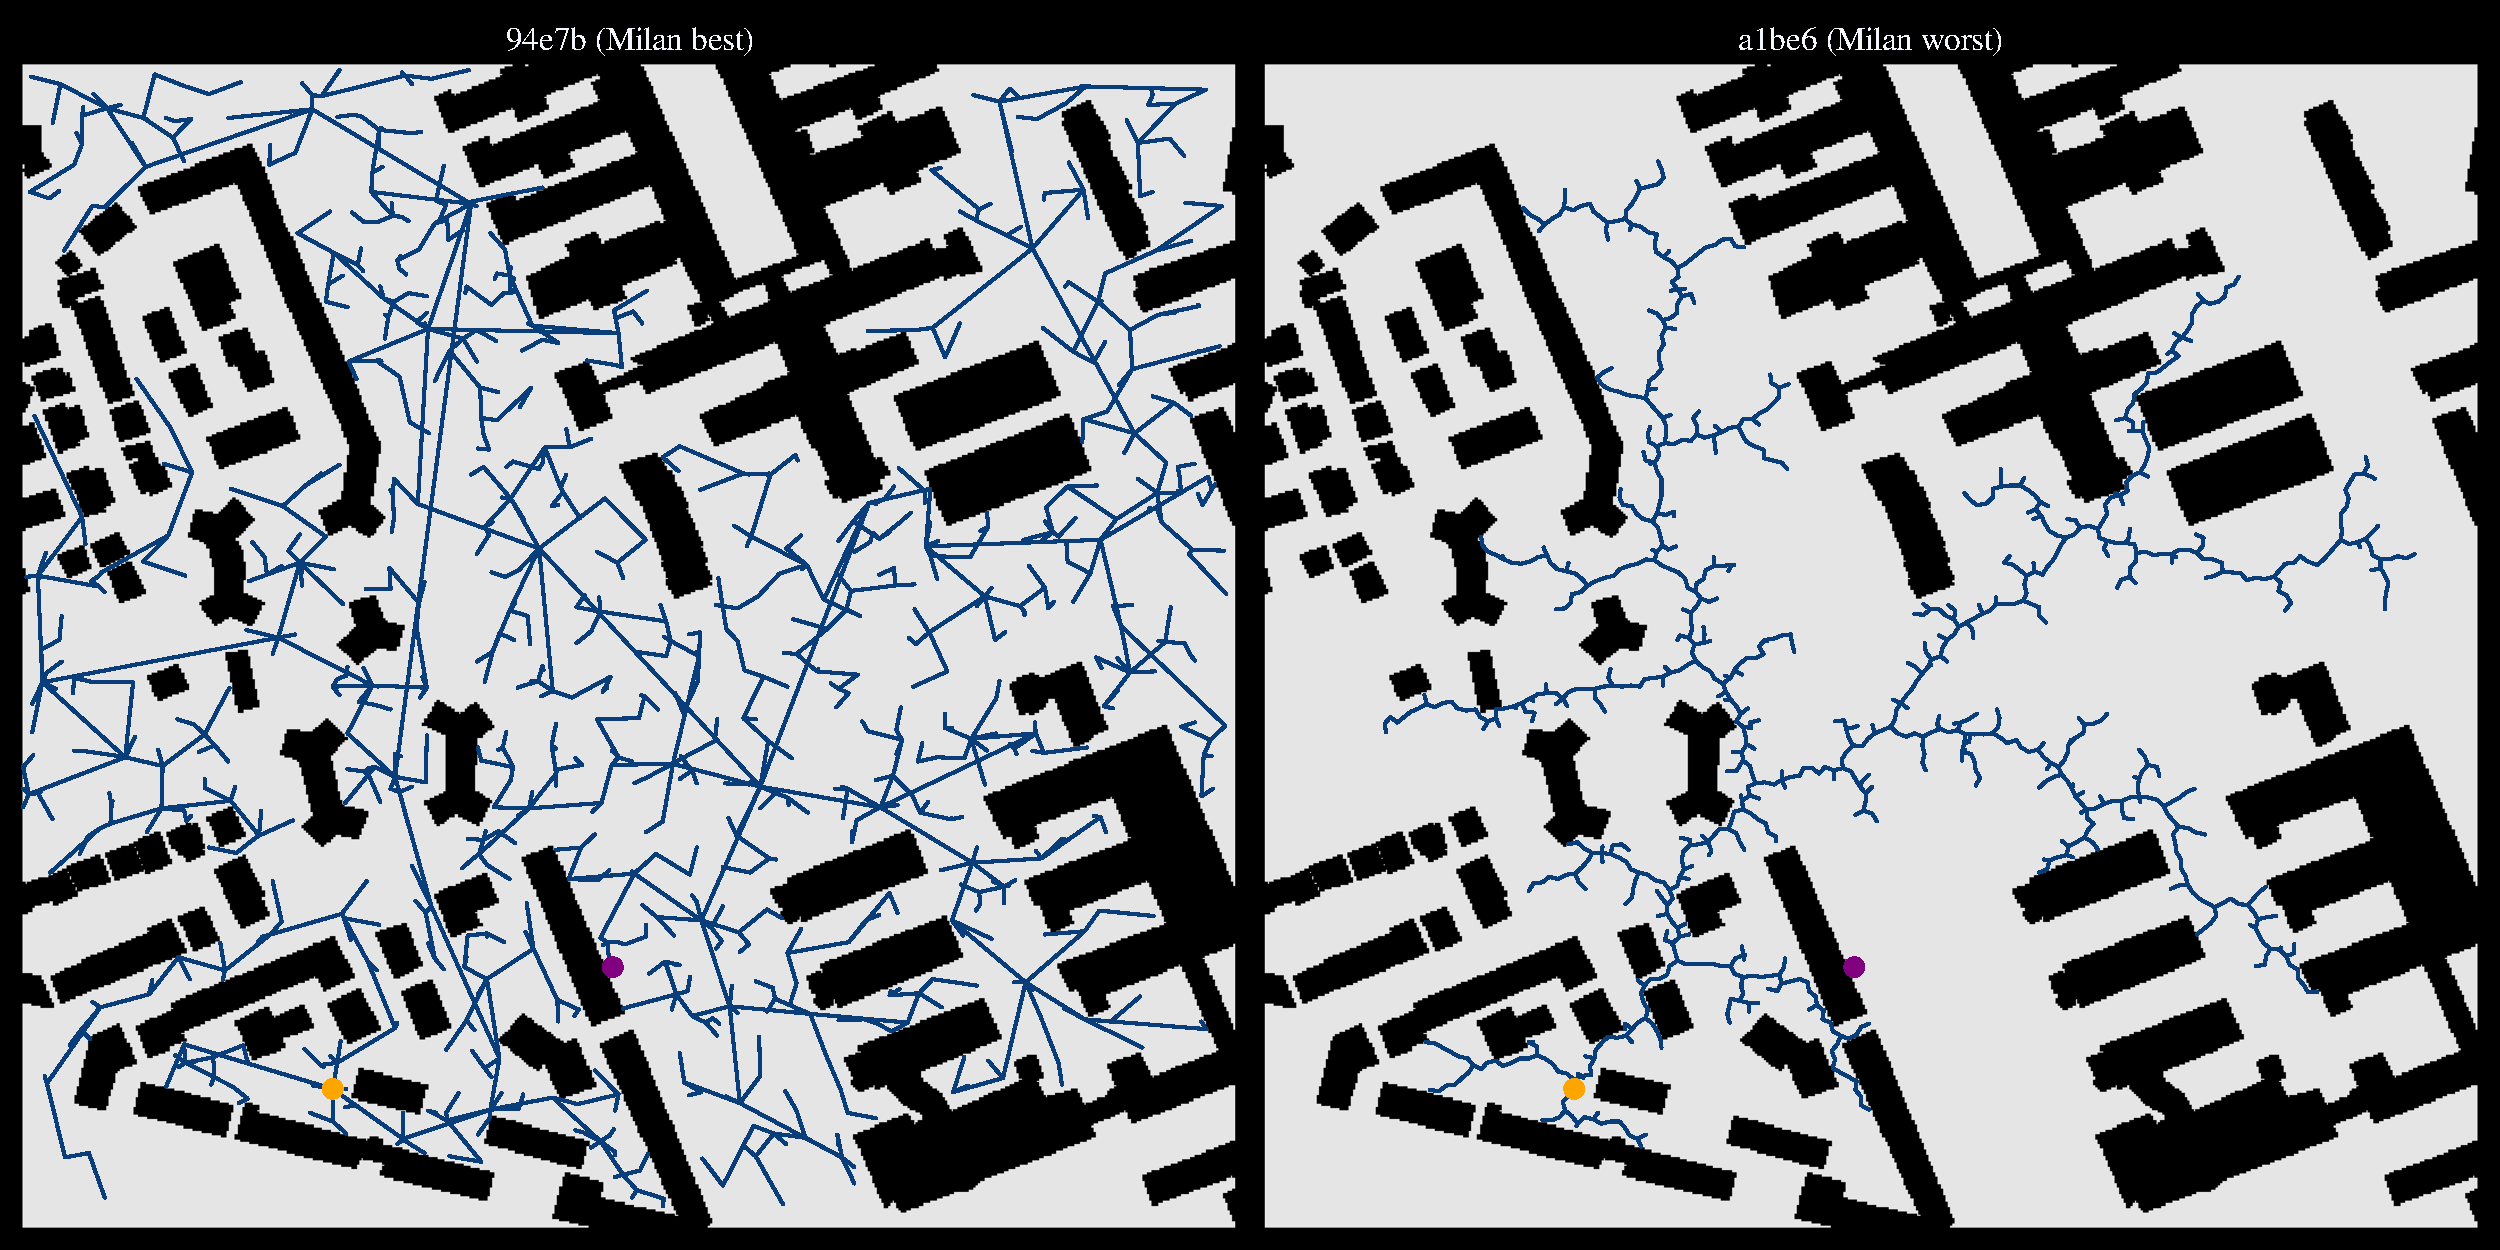
\includegraphics[width=1.0\linewidth, keepaspectratio]{figures/learned_split_0.pdf}
\end{frame}

\begin{frame}{Enigma/Entangle. Convergent Evolution}
    % Next, there is the best planner on the Enigma map, planner 49980, on the left. 
    % This planner biases towards the goal 13% of the time, and considers 75% fewer nodes than the baseline planner.
    % MOST significantly, this planner is exactly the same as planner c5b4f, which
    %   evolved as the best-in-class planner on the Entanglement map. 
    % This is an example of convergent evolution.
    % Finding situations like this is the core goal of this thesis.
    % (pause)
    \centering
    \vspace{-0.1}
    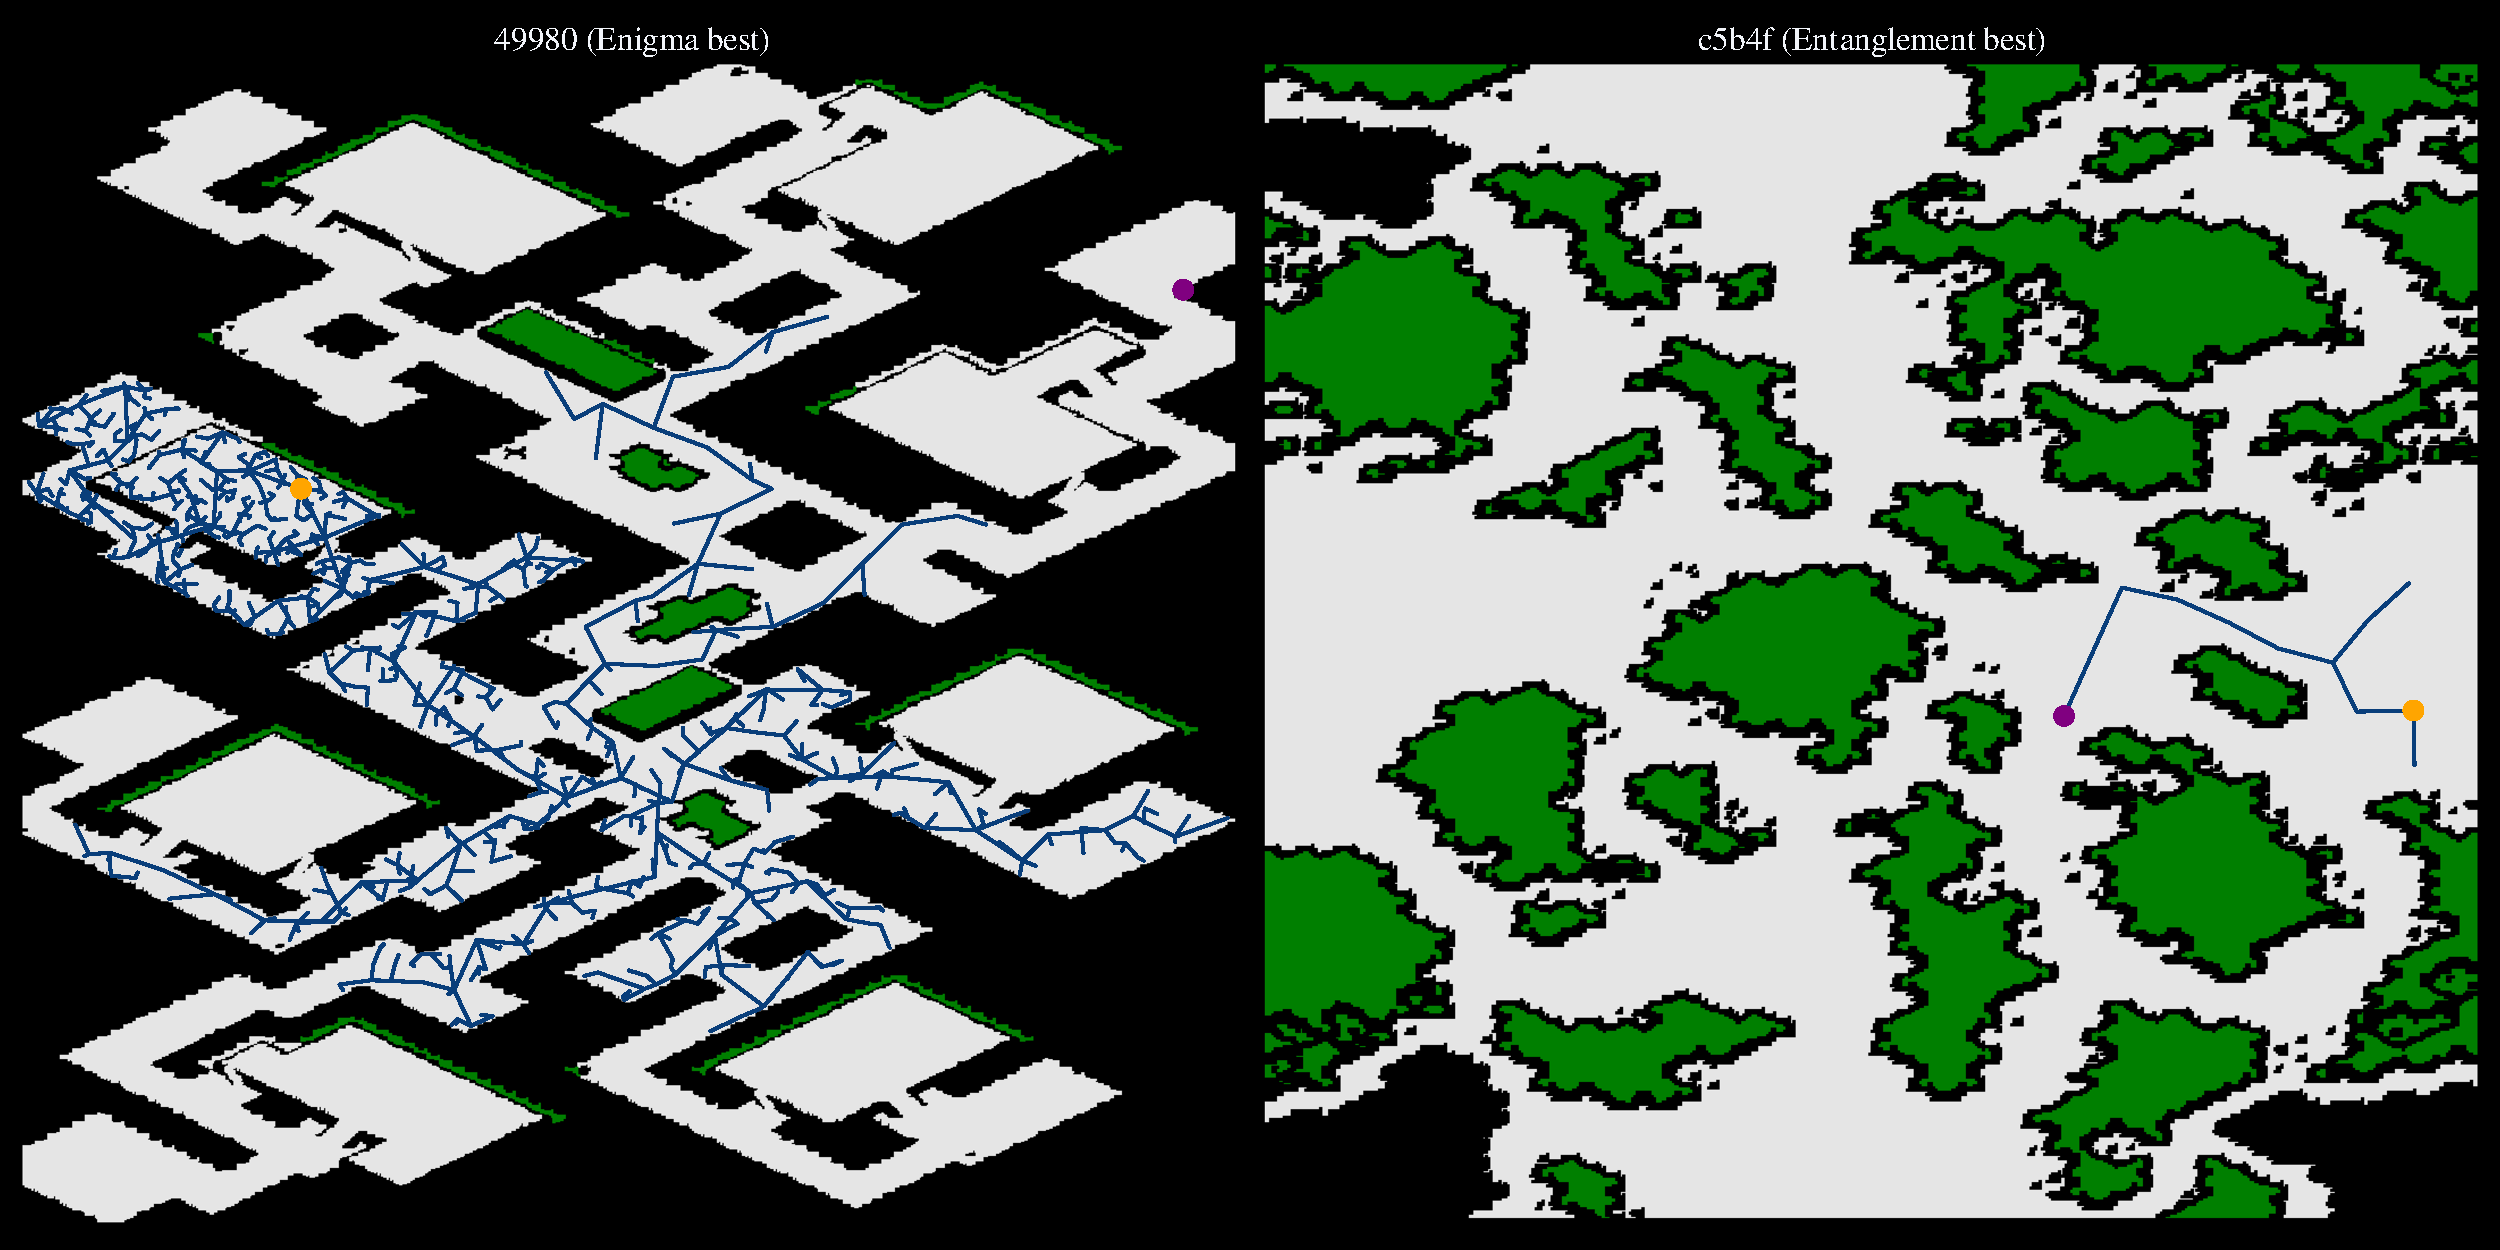
\includegraphics[width=1.0\linewidth, keepaspectratio]{figures/learned_split_1.pdf}
\end{frame}

\begin{frame}{49980 Validation Example}
    % Here is a quick validation run showing how a single attempt differed from the initial baseline.
    % Essentially, it considers fewer nodes and stops early.
    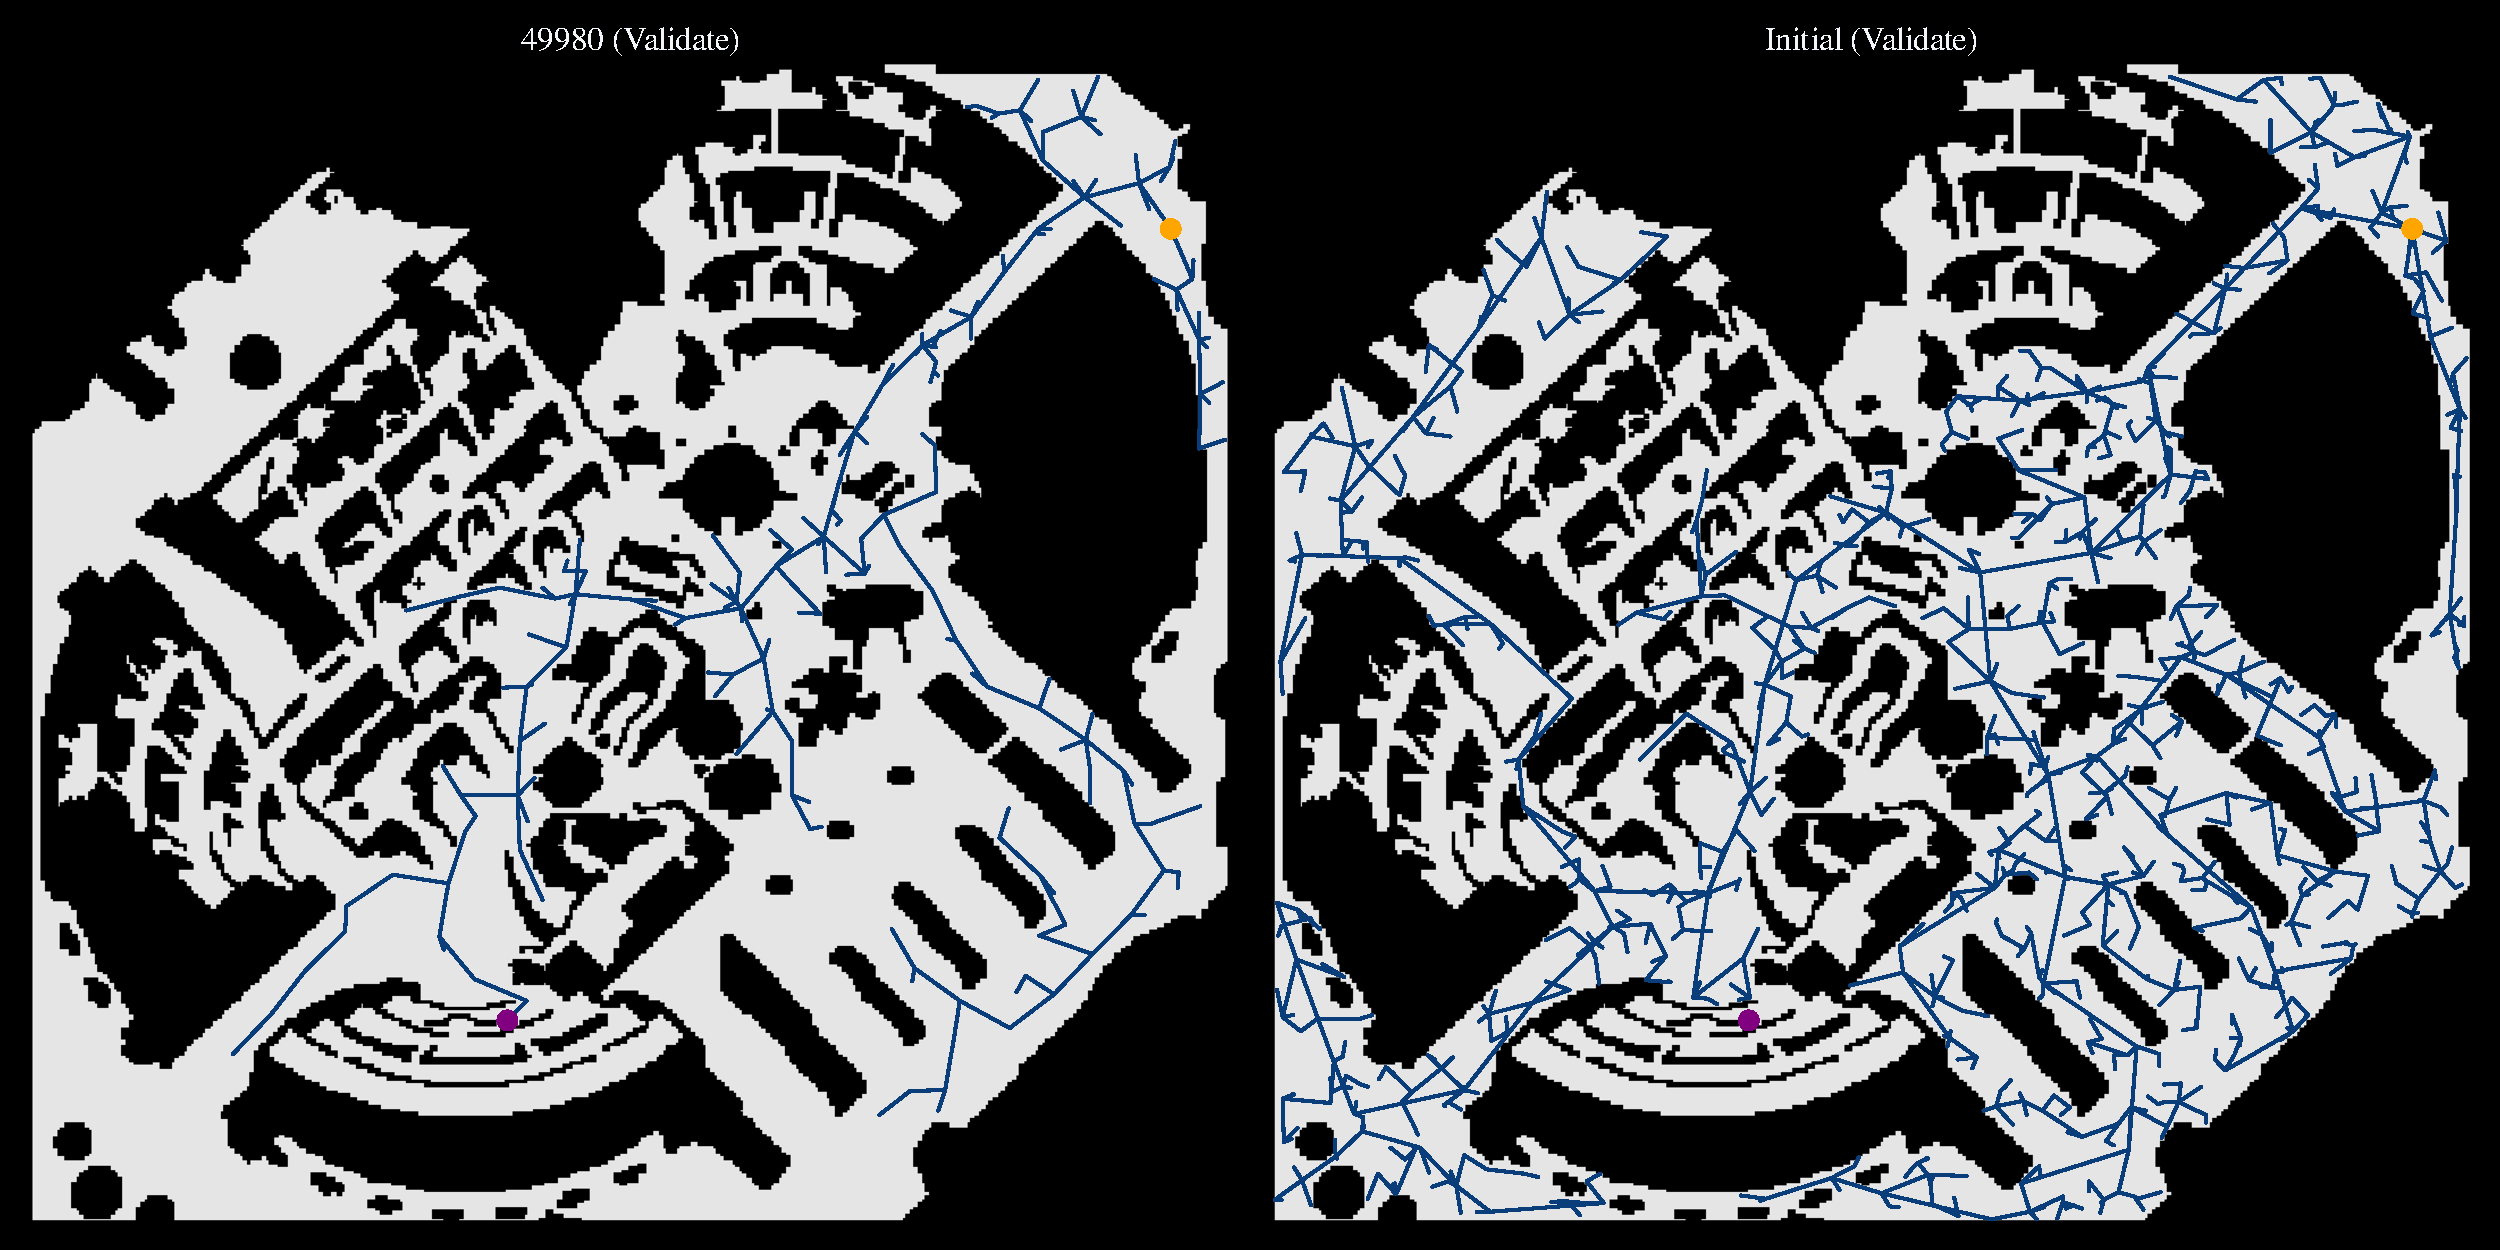
\includegraphics[width=1.0\linewidth, keepaspectratio]{figures/learned_split_2.pdf}
\end{frame}

\begin{frame}{Turbo and No-Obstacles}
    % Alternatively, the Turbo planner learns to bias towards the goal roughly half the time, presumably because the space is so open.
    % Finally, the blank map planner learns to bias 89% of the time, because the open map allows it to do so.
    % This acted as a control for the other experiments
    % These results were the first preliminary indication that goal-specialization was succeeding.
    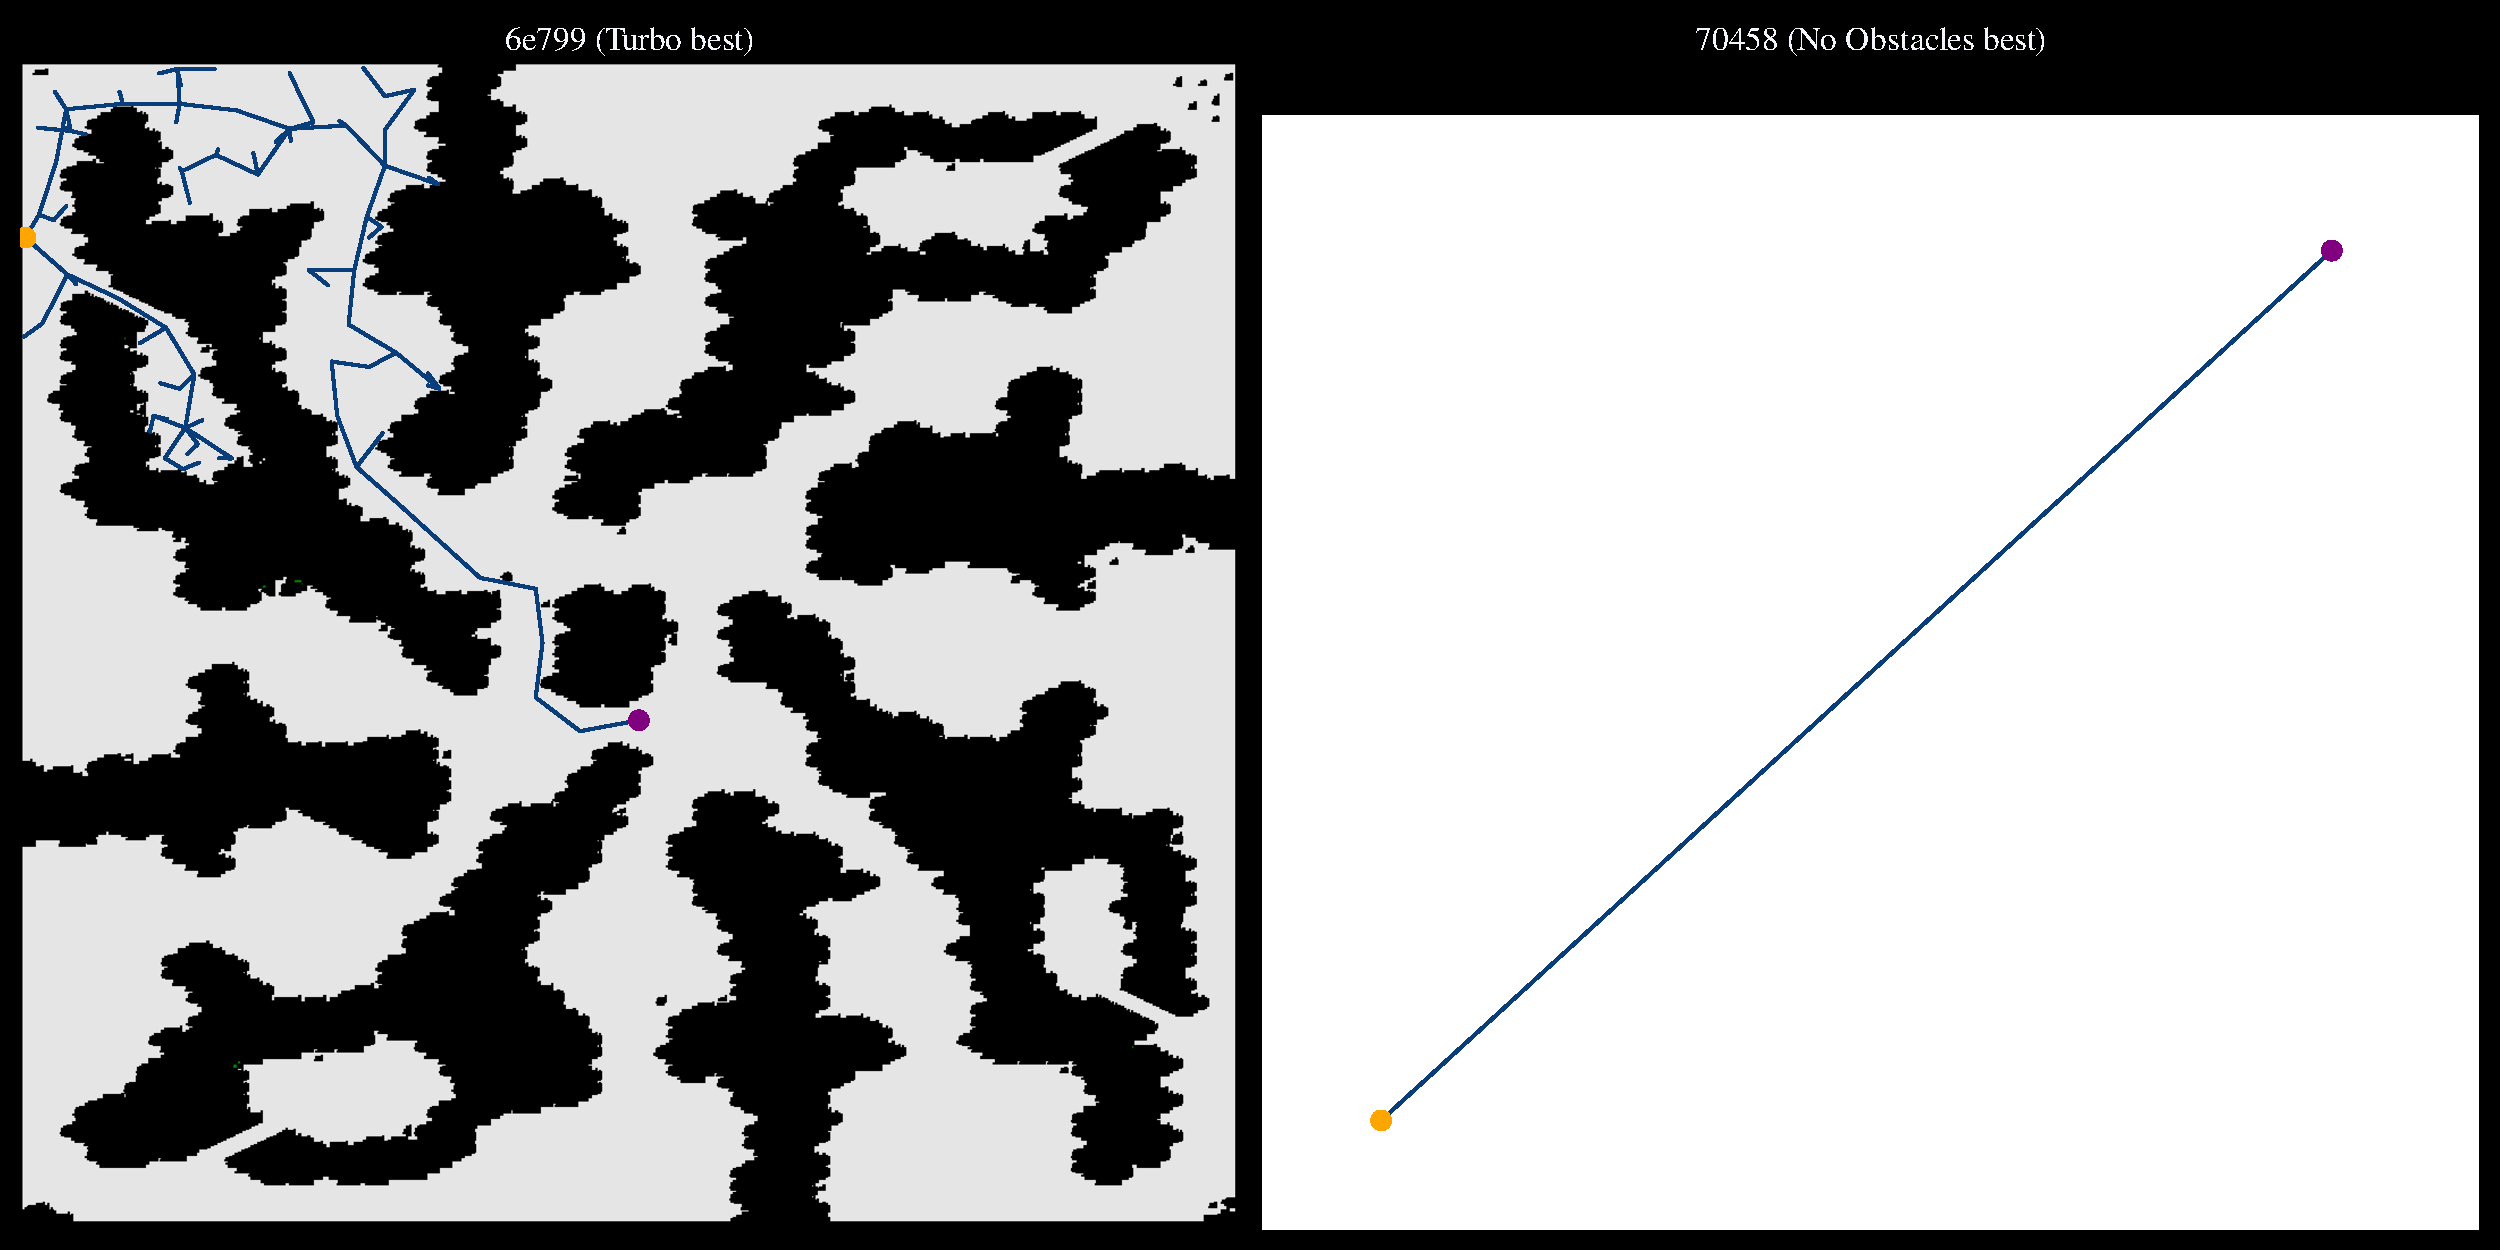
\includegraphics[width=1.0\linewidth, keepaspectratio]{figures/learned_split_3.pdf}
\end{frame}


\begin{frame}{Blank Validation}
    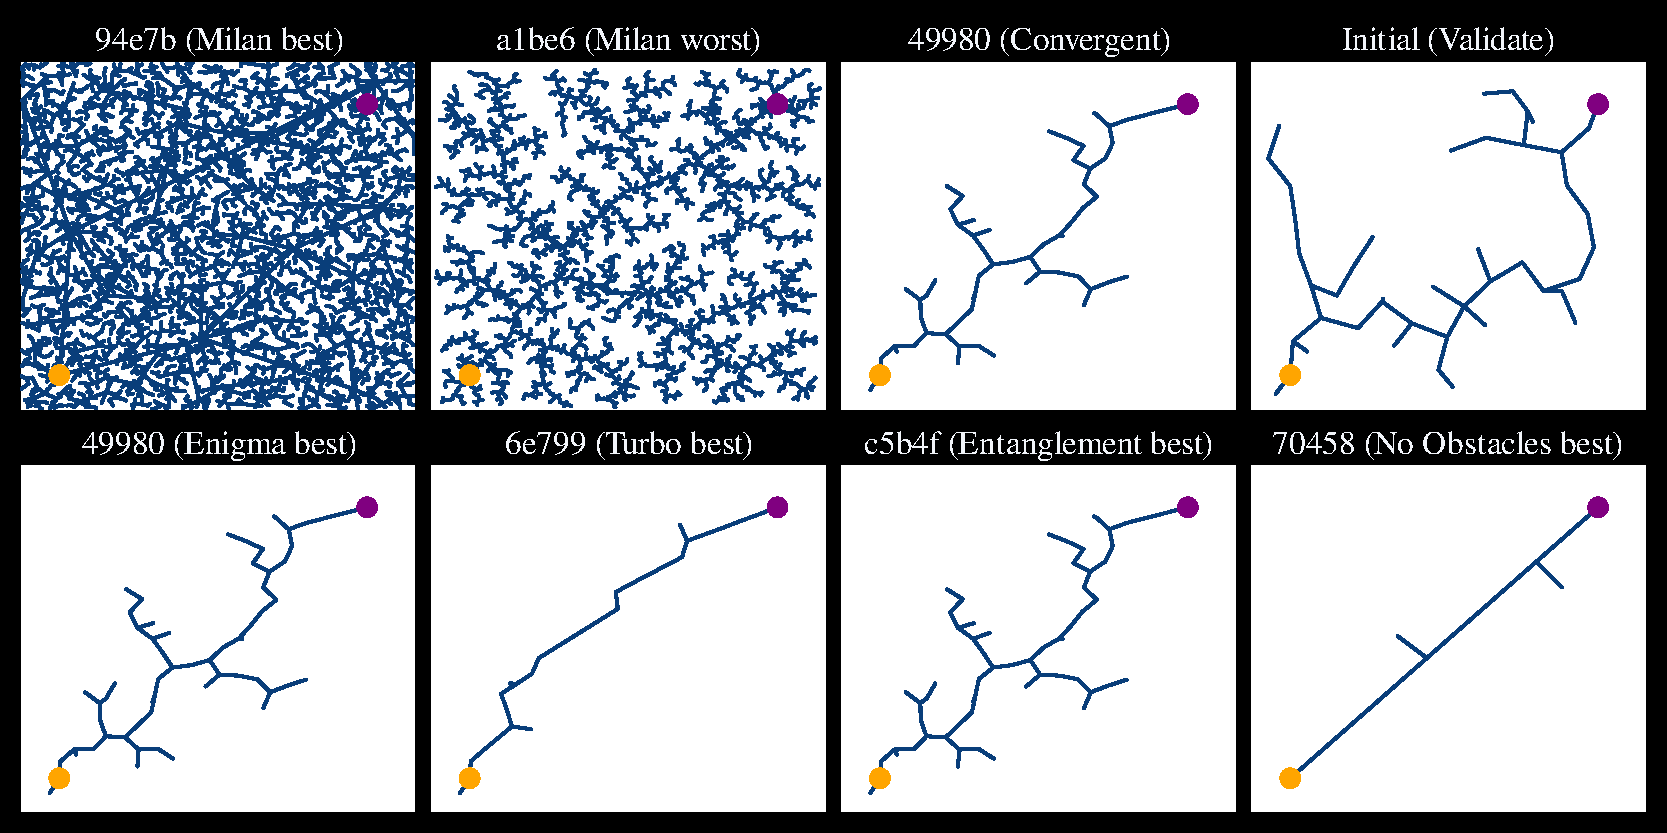
\includegraphics[width=1.0\linewidth, keepaspectratio]{figures/blank_val.pdf}
\end{frame}

% \begin{frame}{Milan Validation}
%     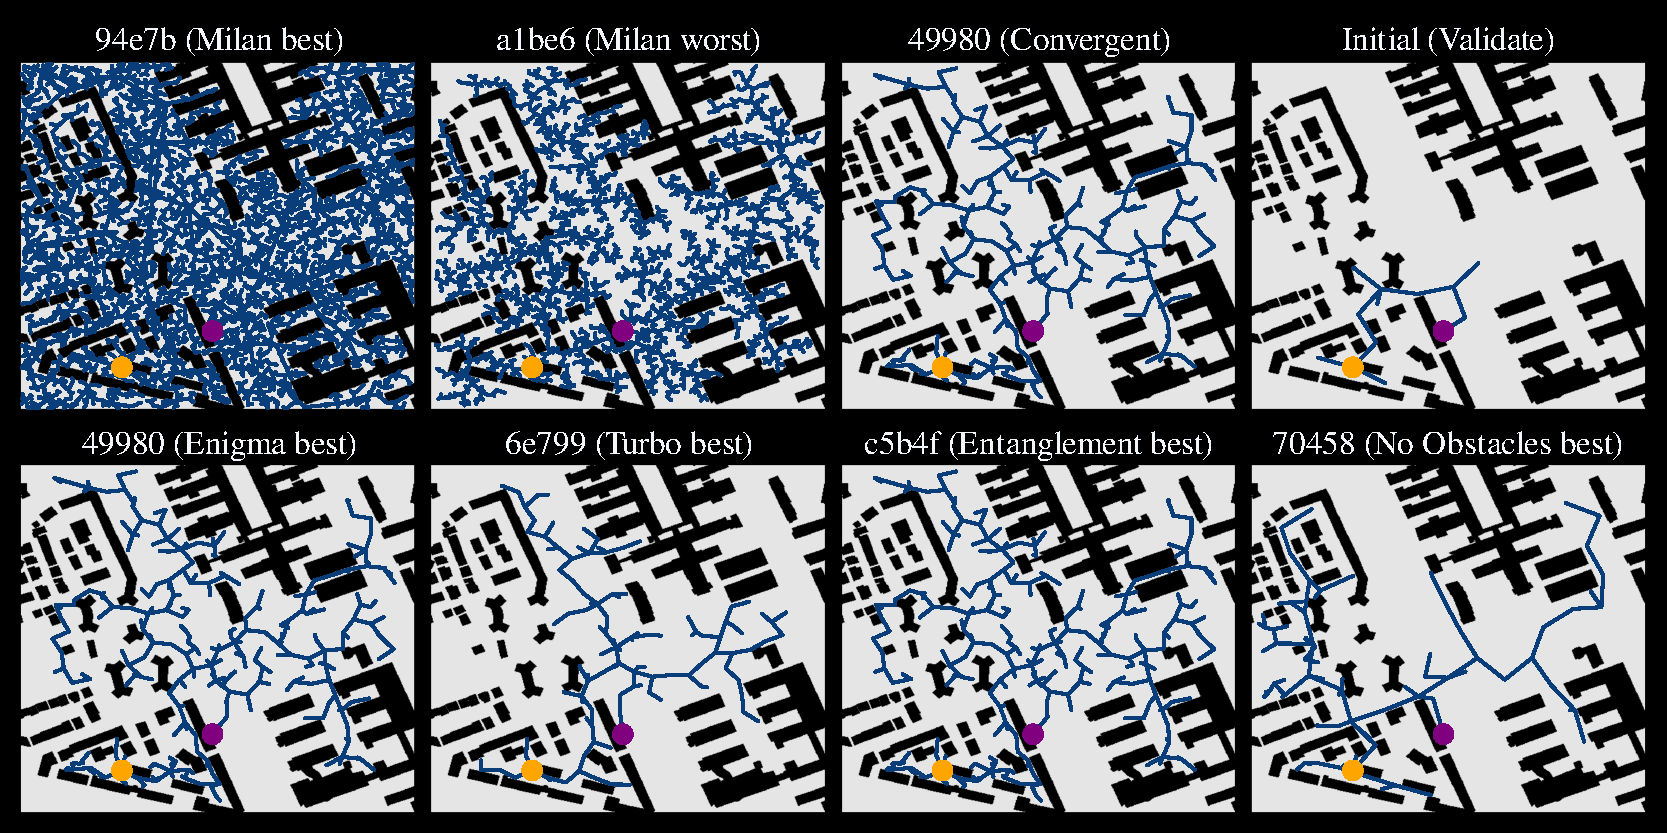
\includegraphics[width=1.0\linewidth, keepaspectratio]{figures/milan_val.pdf}
% \end{frame}
% 
% \begin{frame}{Baldur's Gate Validation}
%     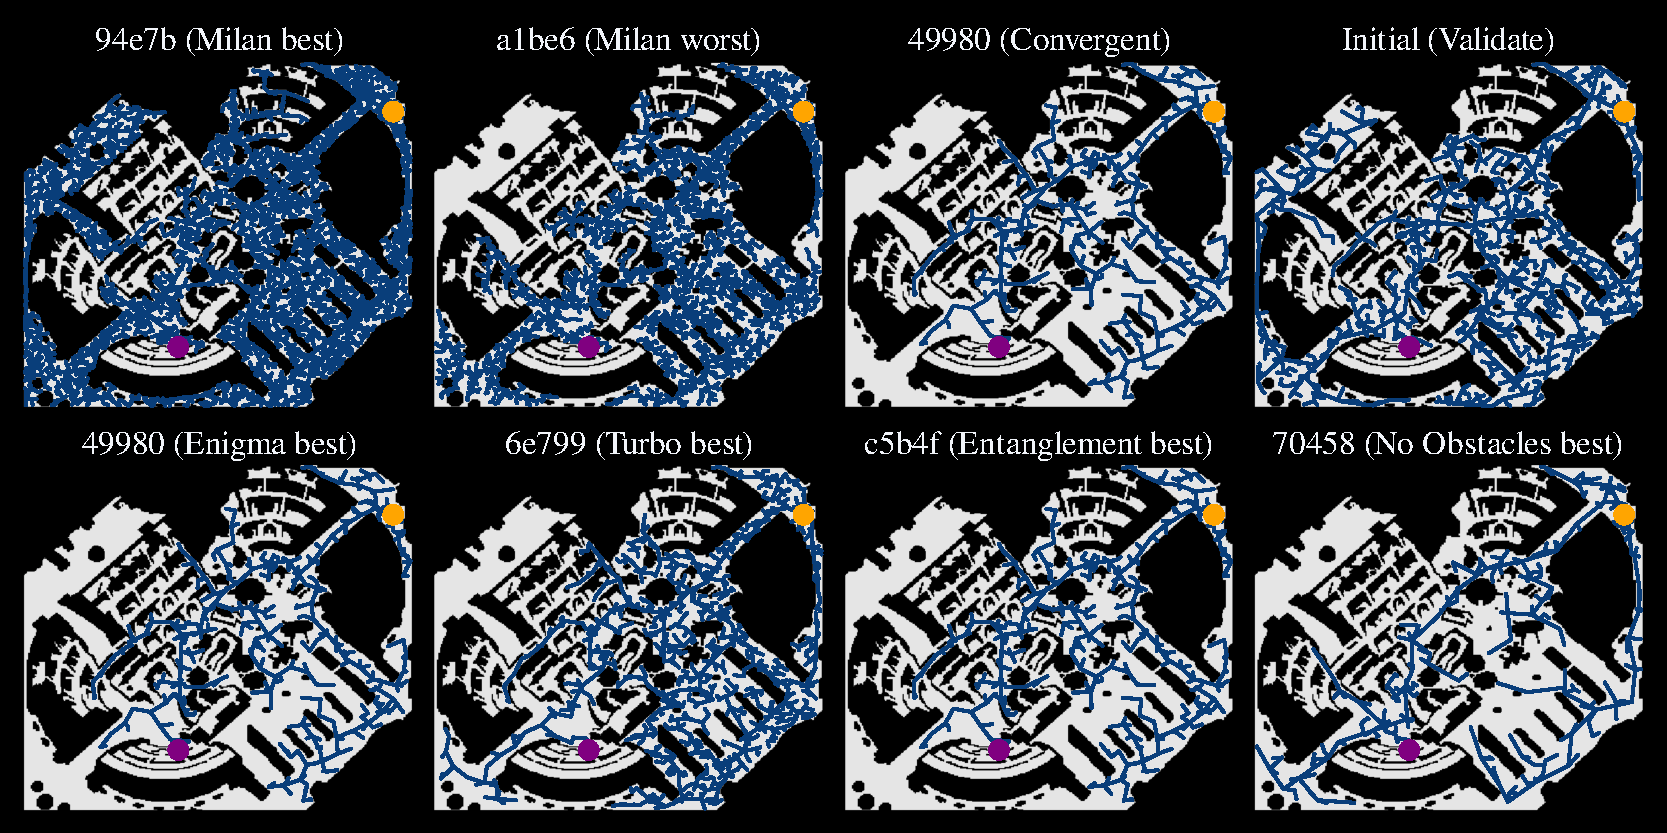
\includegraphics[width=1.0\linewidth, keepaspectratio]{figures/baldurs_val.pdf}
% \end{frame}

{
\setbeamercolor{background canvas}{bg=white}
\begin{frame}[plain]
  % As a reminder, here is an artists depiction of the tree of life
  %   Ideally, we're able to evolve robots, or computer programs, in the same way.
  \begin{figure}
  \centering
  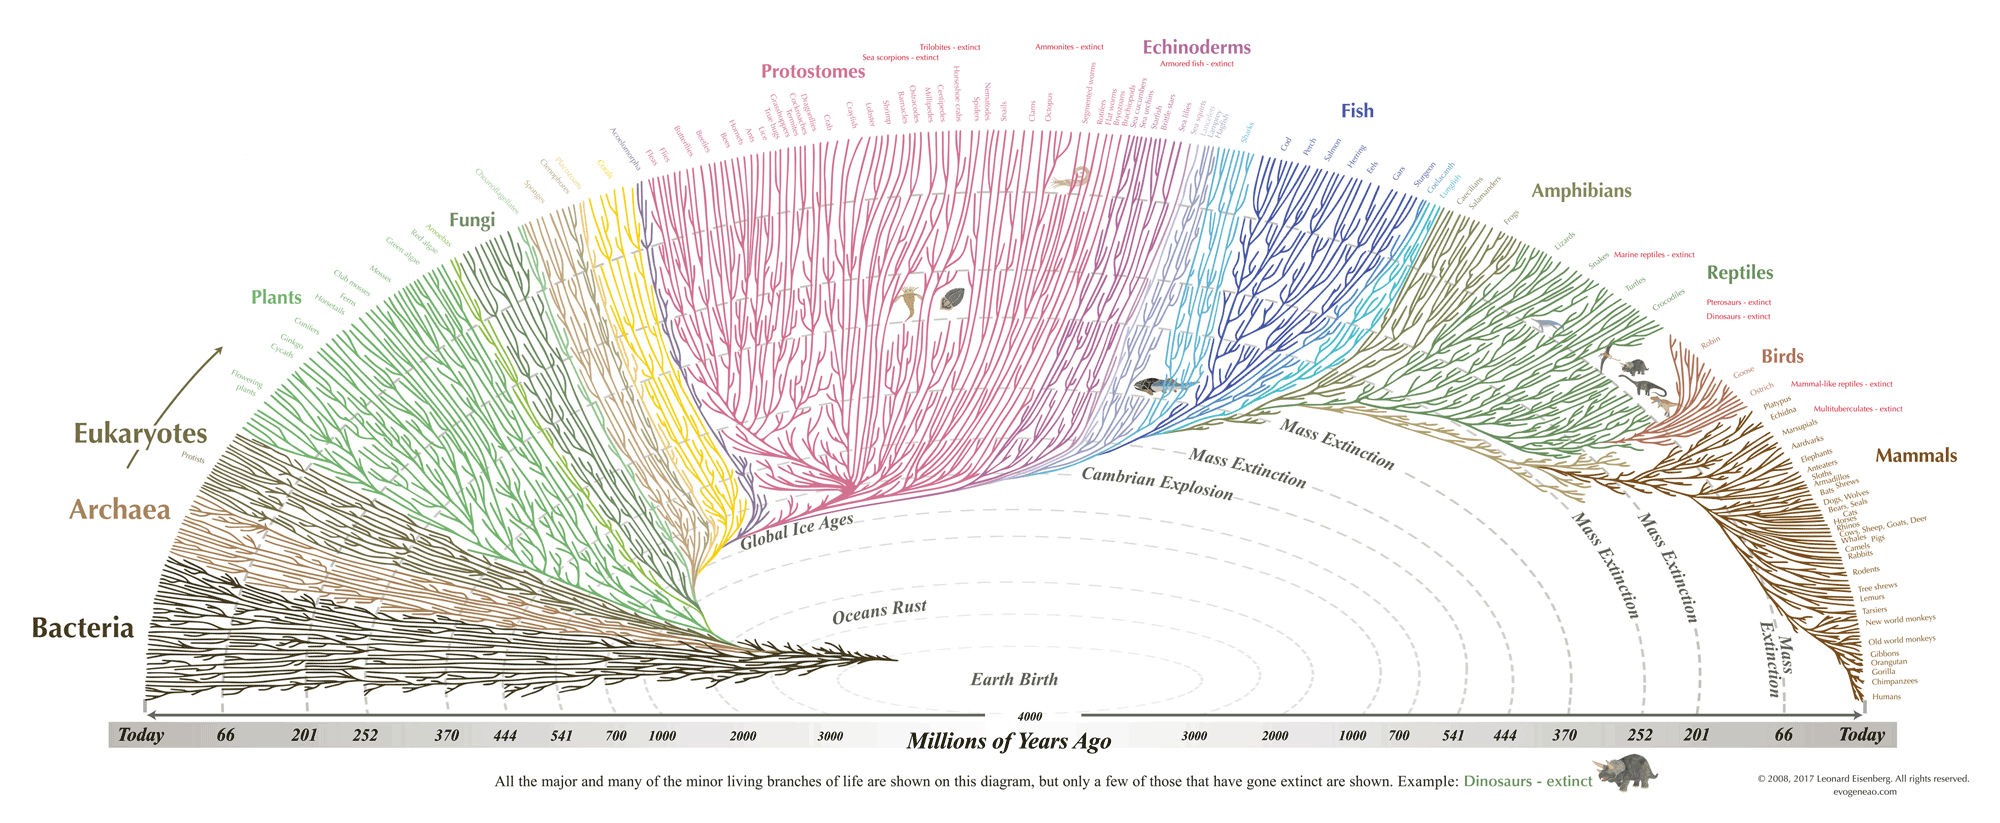
\includegraphics[width=1.0\linewidth,keepaspectratio]{figures/tree_of_life.png}
  \end{figure}
  \begin{center}
      \emphasis{Natural evolution}
  \end{center}
\end{frame}
}

\begin{frame}[plain]
  % So, for instance, how did planner 49980 evolve?
  % This figure shows the ancestry tree for the Starcraft Enigma experiment.
  \begin{figure}
  \centering
  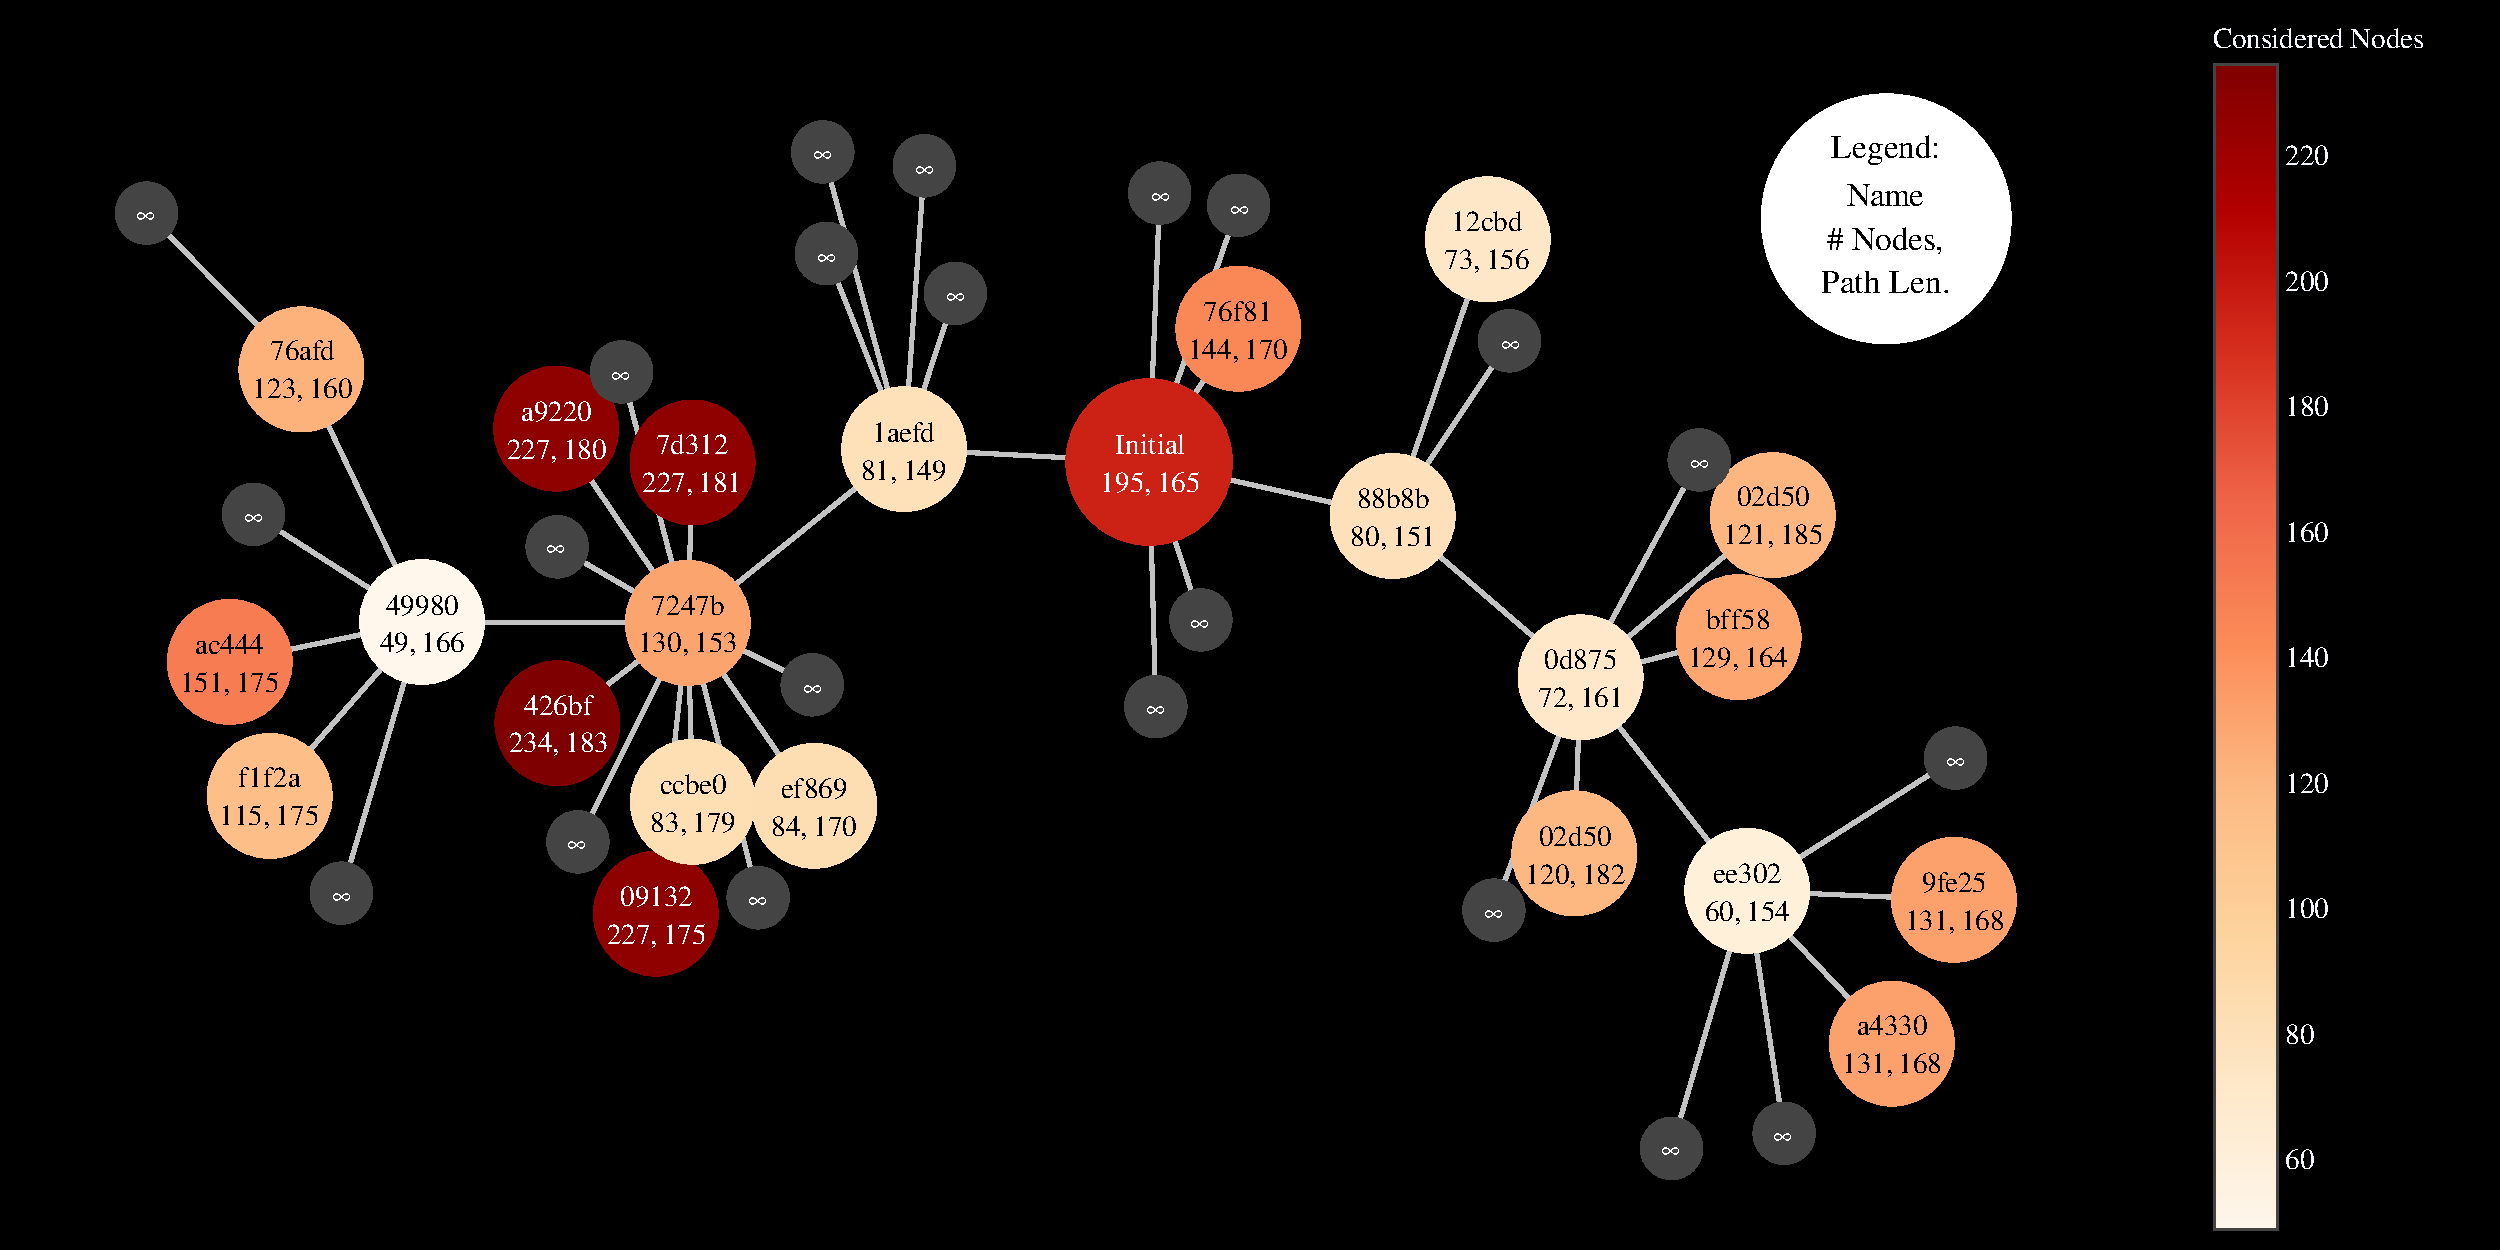
\includegraphics[width=1.0\linewidth,keepaspectratio]{figures/tree.pdf}
  \end{figure}
  \begin{center}
  \emphasis{Evolved Computer Programs}
  \end{center}
\end{frame}


\begin{frame}{Specialization Results}
% This table summarizes the first specialization results across five different maps.
% Each planner reduces the number of nodes that it considers relative to the baseline.
% However, almost every planner does so in a different way.
% The Milan planner modified step size, it was also the hardest to find in terms of Edit Depth
% The Enigma and Entanglement planners modify the bias parameter to 7/8, which controls how likely a planner is to move directly to the goal.
% Interestingly, they were also *found* in identical ways at the same depths.
% They also modify the step size parameter.

% Finally, the Turbo and No Obstacles planners also change the bias parameter, but to different values for each map.
% The no-obstacles planner is found relatively easily, at depth 1.

% Overall, these improvements are significant, but the initial template is easy to improve, and the other conditions of this experiment are also set up to intentionally cause specialization.
\begin{table}[h]
{\small 
\caption{Best-in-class RRT* Statistics (Nodes)}
\label{environments}
\begin{center}
\begin{tabular}{l|lllll}
\hline \hline
\multicolumn{1}{c}{\bf Map}  & 
\multicolumn{1}{c}{\bf $\displaystyle -\Delta$\% Nodes} &  \multicolumn{1}{c}{\bf Edit Depth} &  \multicolumn{1}{c}{\bf Hash} & 
\multicolumn{1}{c}{\bf $r_0$ (step size)} &  \multicolumn{1}{c}{\bf $\alpha$ (bias)} &
% Name                 | Nodes   | Depth | Name | r | a | Path | Depth | Name | r | a
Milan        & \cc{$82.35$\%} & $4$ & \plnr{94e7b}  & \cb{$50,000$} & \gr{$7/4$ (>1)} \\
Enigma       & \cc{$74.87$\%} & $3$ & \plnr{49980}  & \cb{$100$}    & \cb{$7/8$} \\
Entanglement & \cc{$85.16$\%} & $3$ & \plnr{c5b4f}  & \cb{$100$}    & \cb{$7/8$} \\
Turbo        & \cc{$64.29$\%} & $3$ & \plnr{6e799}  & \gr{$50$}     & \cb{$4/9$} \\
No Obstacles & \cc{$89.47$\%} & $1$ & \plnr{70458}  & \gr{$50$} & \cb{$1/9$} \\
\hline 
\multicolumn{1}{c}{\bf Baseline} & \gr{$0.0$\%} & $0$ & {\color{code}Initial}  & \gr{$50$}     & \gr{$1.0$} \\
\hline \hline
\end{tabular}
\end{center}}
\end{table}
\end{frame}

\begin{frame}{Efficient Exploration}
    \centering
    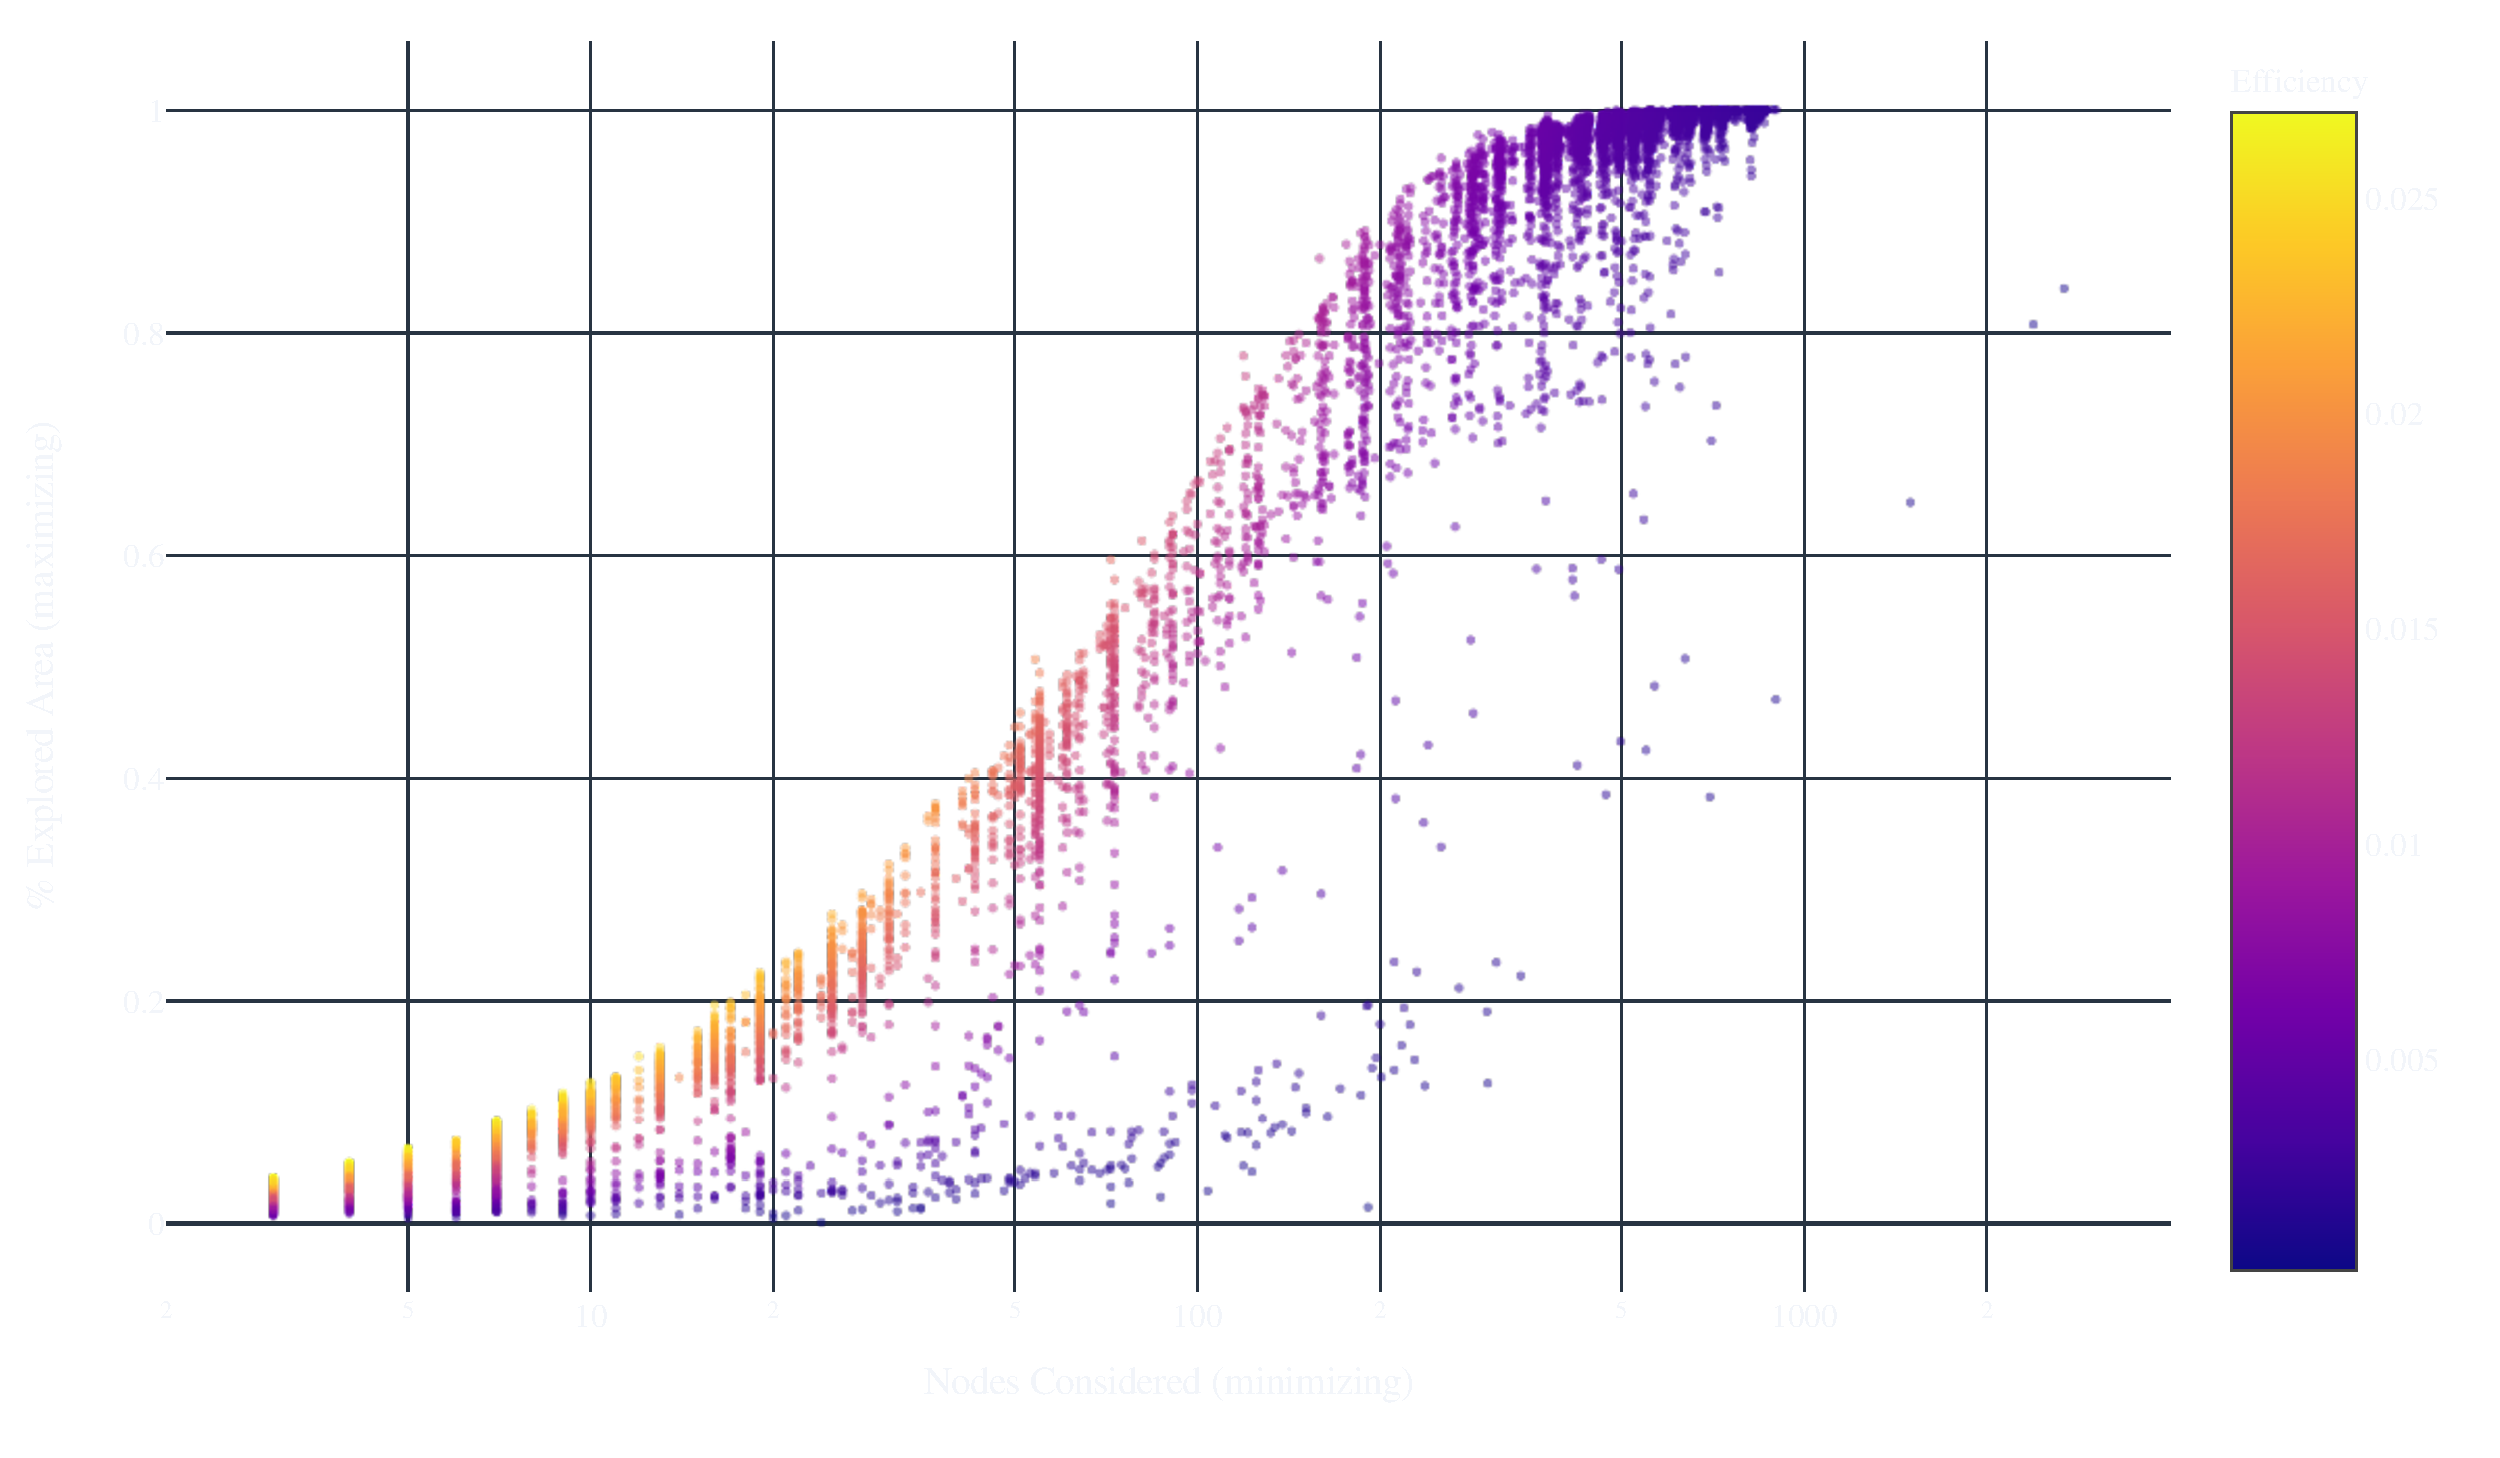
\includegraphics[width=0.85\linewidth, keepaspectratio]{figures/efficient_overview.pdf}
\end{frame}

\begin{frame}{\white{Experiment Types}}
    \begin{vfilleditems}
    \item \emphasis{Improve}
    \item \emphasis{Select}
    \item \emphasis{Fix}
    \end{vfilleditems}
\end{frame}

\begin{frame}{\white{Future Work}}
    \begin{vfilleditems}
    \item \emphasis{Algorithms} 
    \item \emphasis{Environments} 
    \item \emphasis{Optimization} 
    \end{vfilleditems}
\end{frame}

\begin{frame}{Program Learning Template}
\begin{table}[h]
{\small 
\caption{Program Learning Problems}
\label{environments}
\begin{center}
\begin{tabular}{l|lllll}
\hline \hline
\multicolumn{1}{c}{\bf \cb{Problem}}  & 
\multicolumn{1}{c}{\bf \cc{Representation}} &  
\multicolumn{1}{c}{\bf \ce{Optimization}} \\  
\hline
Image Classification & NN Weights              & Gradient \\
Char. Recognition    & Probabilistic Program   & Bayes. Inference \\
Arch. Search         & Tensor Register Machine & Regularized Evolution \\
Path Planning    & Python Program          & Pareto Evolution \\
\hline \hline
\end{tabular}
\end{center}}
\end{table}
\begin{figure}
    \centering
    \begin{overpic}[width=0.45\linewidth, keepaspectratio]{figures/meme4.jpg}
        \put(-40,35){\Medium Wait, it's all}
        \put(-40,28){\Medium program}
        \put(-40,21){\Medium learning?}
        \put(105,30){\Medium \red{Always has been.}}
    \end{overpic}
\end{figure}
\end{frame}

\begin{frame}[plain]{}
    \centering
    \vfill
    {\fontsize{40}{50}\selectfont \red{No Free Lunch}}
    \vfill
\end{frame}

\appendix % do not count the following slides for the total number
\section*{Backup Slides}

\begin{frame}[plain, noframenumbering]
  \centering
  \vfill
  {\fontsize{40}{50}\selectfont Questions?}
  \vfill
\end{frame}

\begin{frame}{Research Questions}
  \begin{vfilleditems}
    \item {\Huge Are these research questions? {\color{pureminimalistic@text@red} Answer.}}
    % TODO: Answer each at high level
    {\color{grey}
    \item {\Huge Is crossover necessary?}
    \item {\Huge What is the role of latent code?}
    \item {\Huge How should code be mutated?}
    \item {\Huge How hard is a problem?}
    }
  \end{vfilleditems}
\end{frame}

\begin{frame}{Research Questions}
  \begin{vfilleditems}
    \item {\Huge Role of program representation?}
    \item {\Huge Role of scale and compute efficiency?}
    \item {\Huge How should code be mutated?}
    \item {\Huge How hard is a problem?}
  \end{vfilleditems}
\end{frame}

\begin{frame}{Challenges Faced}
    \begin{vfilleditems}
    \item \Huge Test
    \end{vfilleditems}
\end{frame}

\begin{frame}{Gritty Engineering Work}
    \begin{vfilleditems}
    \item \Huge Test
    \end{vfilleditems}
\end{frame}

\begin{frame}[plain, noframenumbering]
  \centering
  \printbibliography
\end{frame}

\end{document}
